\documentclass{book}
\usepackage[a4paper,top=2.5cm,bottom=2.5cm,left=2.5cm,right=2.5cm]{geometry}
\usepackage{makeidx}
\usepackage{natbib}
\usepackage{graphicx}
\usepackage{multicol}
\usepackage{float}
\usepackage{listings}
\usepackage{color}
\usepackage{ifthen}
\usepackage[table]{xcolor}
\usepackage{textcomp}
\usepackage{alltt}
\usepackage{ifpdf}
\ifpdf
\usepackage[pdftex,
            pagebackref=true,
            colorlinks=true,
            linkcolor=blue,
            unicode
           ]{hyperref}
\else
\usepackage[ps2pdf,
            pagebackref=true,
            colorlinks=true,
            linkcolor=blue,
            unicode
           ]{hyperref}
\usepackage{pspicture}
\fi
\usepackage[utf8]{inputenc}
\usepackage{mathptmx}
\usepackage[scaled=.90]{helvet}
\usepackage{courier}
\usepackage{sectsty}
\usepackage{amssymb}
\usepackage[titles]{tocloft}
\usepackage{doxygen}
\lstset{language=C++,inputencoding=utf8,basicstyle=\footnotesize,breaklines=true,breakatwhitespace=true,tabsize=4,numbers=left }
\makeindex
\setcounter{tocdepth}{3}
\renewcommand{\footrulewidth}{0.4pt}
\renewcommand{\familydefault}{\sfdefault}
\hfuzz=15pt
\setlength{\emergencystretch}{15pt}
\hbadness=750
\tolerance=750
\begin{document}
\hypersetup{pageanchor=false,citecolor=blue}
\begin{titlepage}
\vspace*{7cm}
\begin{center}
{\Large Ensemble Clustering }\\
\vspace*{1cm}
{\large Generated by Doxygen 1.8.2}\\
\vspace*{0.5cm}
{\small Wed Oct 17 2012 16:55:35}\\
\end{center}
\end{titlepage}
\clearemptydoublepage
\pagenumbering{roman}
\tableofcontents
\clearemptydoublepage
\pagenumbering{arabic}
\hypersetup{pageanchor=true,citecolor=blue}
\chapter{Namespace Index}
\section{Namespace List}
Here is a list of all namespaces with brief descriptions\-:\begin{DoxyCompactList}
\item\contentsline{section}{\hyperlink{namespace_aux}{Aux} }{\pageref{namespace_aux}}{}
\item\contentsline{section}{\hyperlink{namespace_networ_kit}{Networ\-Kit} }{\pageref{namespace_networ_kit}}{}
\item\contentsline{section}{\hyperlink{namespace_option_parser}{Option\-Parser} \\*The namespace of The Lean Mean C++ \hyperlink{class_option_parser_1_1_option}{Option} \hyperlink{class_option_parser_1_1_parser}{Parser} }{\pageref{namespace_option_parser}}{}
\end{DoxyCompactList}

\chapter{Hierarchical Index}
\section{Class Hierarchy}
This inheritance list is sorted roughly, but not completely, alphabetically\-:\begin{DoxyCompactList}
\item \contentsline{section}{Option\-Parser\-:\-:Parser\-:\-:Action}{\pageref{struct_option_parser_1_1_parser_1_1_action}}{}
\begin{DoxyCompactList}
\item \contentsline{section}{Option\-Parser\-:\-:Parser\-:\-:Store\-Option\-Action}{\pageref{class_option_parser_1_1_parser_1_1_store_option_action}}{}
\item \contentsline{section}{Option\-Parser\-:\-:Stats\-:\-:Count\-Options\-Action}{\pageref{class_option_parser_1_1_stats_1_1_count_options_action}}{}
\end{DoxyCompactList}
\item \contentsline{section}{Option\-Parser\-:\-:Arg}{\pageref{struct_option_parser_1_1_arg}}{}
\begin{DoxyCompactList}
\item \contentsline{section}{Arg}{\pageref{class_arg}}{}
\end{DoxyCompactList}
\item \contentsline{section}{Networ\-Kit\-:\-:Clusterer}{\pageref{class_networ_kit_1_1_clusterer}}{}
\begin{DoxyCompactList}
\item \contentsline{section}{Networ\-Kit\-:\-:Ensemble\-Multilevel}{\pageref{class_networ_kit_1_1_ensemble_multilevel}}{}
\item \contentsline{section}{Networ\-Kit\-:\-:Ensemble\-Preprocessing}{\pageref{class_networ_kit_1_1_ensemble_preprocessing}}{}
\item \contentsline{section}{Networ\-Kit\-:\-:Label\-Propagation}{\pageref{class_networ_kit_1_1_label_propagation}}{}
\item \contentsline{section}{Networ\-Kit\-:\-:Louvain}{\pageref{class_networ_kit_1_1_louvain}}{}
\item \contentsline{section}{Networ\-Kit\-:\-:Parallel\-Agglomerative\-Clusterer}{\pageref{class_networ_kit_1_1_parallel_agglomerative_clusterer}}{}
\item \contentsline{section}{Networ\-Kit\-:\-:Random\-Clusterer}{\pageref{class_networ_kit_1_1_random_clusterer}}{}
\end{DoxyCompactList}
\item \contentsline{section}{Networ\-Kit\-:\-:Clustering\-Generator}{\pageref{class_networ_kit_1_1_clustering_generator}}{}
\item \contentsline{section}{Networ\-Kit\-:\-:Clustering\-Projector}{\pageref{class_networ_kit_1_1_clustering_projector}}{}
\item \contentsline{section}{Networ\-Kit\-:\-:Clustering\-Reader}{\pageref{class_networ_kit_1_1_clustering_reader}}{}
\item \contentsline{section}{Networ\-Kit\-:\-:Clustering\-Writer}{\pageref{class_networ_kit_1_1_clustering_writer}}{}
\item \contentsline{section}{Networ\-Kit\-:\-:Contracter}{\pageref{class_networ_kit_1_1_contracter}}{}
\begin{DoxyCompactList}
\item \contentsline{section}{Networ\-Kit\-:\-:Cluster\-Contracter}{\pageref{class_networ_kit_1_1_cluster_contracter}}{}
\item \contentsline{section}{Networ\-Kit\-:\-:Matching\-Contracter}{\pageref{class_networ_kit_1_1_matching_contracter}}{}
\end{DoxyCompactList}
\item \contentsline{section}{C\-S\-V\-Writer}{\pageref{class_c_s_v_writer}}{}
\item \contentsline{section}{Option\-Parser\-:\-:Descriptor}{\pageref{struct_option_parser_1_1_descriptor}}{}
\item \contentsline{section}{Networ\-Kit\-:\-:Dissimilarity\-Measure}{\pageref{class_networ_kit_1_1_dissimilarity_measure}}{}
\begin{DoxyCompactList}
\item \contentsline{section}{Networ\-Kit\-:\-:Jaccard\-Measure}{\pageref{class_networ_kit_1_1_jaccard_measure}}{}
\item \contentsline{section}{Networ\-Kit\-:\-:Rand\-Measure}{\pageref{class_networ_kit_1_1_rand_measure}}{}
\end{DoxyCompactList}
\item \contentsline{section}{Networ\-Kit\-:\-:Graph\-:\-:Edge\-Attribute}{\pageref{class_networ_kit_1_1_graph_1_1_edge_attribute}}{}
\item \contentsline{section}{Networ\-Kit\-:\-:Edge\-Scoring$<$ T $>$}{\pageref{class_networ_kit_1_1_edge_scoring}}{}
\begin{DoxyCompactList}
\item \contentsline{section}{Networ\-Kit\-:\-:Modularity\-Scoring$<$ T $>$}{\pageref{class_networ_kit_1_1_modularity_scoring}}{}
\end{DoxyCompactList}
\item \contentsline{section}{Networ\-Kit\-:\-:Graph}{\pageref{class_networ_kit_1_1_graph}}{}
\item \contentsline{section}{Networ\-Kit\-:\-:Graph\-Contraction}{\pageref{class_networ_kit_1_1_graph_contraction}}{}
\item \contentsline{section}{Networ\-Kit\-:\-:Graph\-Generator}{\pageref{class_networ_kit_1_1_graph_generator}}{}
\item \contentsline{section}{Networ\-Kit\-:\-:Graph\-I\-O}{\pageref{class_networ_kit_1_1_graph_i_o}}{}
\item \contentsline{section}{Networ\-Kit\-:\-:Graph\-Reader}{\pageref{class_networ_kit_1_1_graph_reader}}{}
\begin{DoxyCompactList}
\item \contentsline{section}{Networ\-Kit\-:\-:M\-E\-T\-I\-S\-Graph\-Reader}{\pageref{class_networ_kit_1_1_m_e_t_i_s_graph_reader}}{}
\end{DoxyCompactList}
\item \contentsline{section}{Networ\-Kit\-:\-:Graph\-Writer}{\pageref{class_networ_kit_1_1_graph_writer}}{}
\begin{DoxyCompactList}
\item \contentsline{section}{Networ\-Kit\-:\-:M\-E\-T\-I\-S\-Graph\-Writer}{\pageref{class_networ_kit_1_1_m_e_t_i_s_graph_writer}}{}
\end{DoxyCompactList}
\item \contentsline{section}{Networ\-Kit\-:\-:Independent\-Set\-Finder}{\pageref{class_networ_kit_1_1_independent_set_finder}}{}
\begin{DoxyCompactList}
\item \contentsline{section}{Networ\-Kit\-:\-:Luby}{\pageref{class_networ_kit_1_1_luby}}{}
\end{DoxyCompactList}
\item \contentsline{section}{Networ\-Kit\-:\-:Index\-Map$<$ I, T $>$}{\pageref{class_networ_kit_1_1_index_map}}{}
\item \contentsline{section}{Networ\-Kit\-:\-:Index\-Map$<$ node, cluster $>$}{\pageref{class_networ_kit_1_1_index_map}}{}
\begin{DoxyCompactList}
\item \contentsline{section}{Networ\-Kit\-:\-:Node\-Map$<$ cluster $>$}{\pageref{class_networ_kit_1_1_node_map}}{}
\begin{DoxyCompactList}
\item \contentsline{section}{Networ\-Kit\-:\-:Clustering}{\pageref{class_networ_kit_1_1_clustering}}{}
\end{DoxyCompactList}
\end{DoxyCompactList}
\item \contentsline{section}{Networ\-Kit\-:\-:Index\-Map$<$ node, node $>$}{\pageref{class_networ_kit_1_1_index_map}}{}
\begin{DoxyCompactList}
\item \contentsline{section}{Networ\-Kit\-:\-:Node\-Map$<$ node $>$}{\pageref{class_networ_kit_1_1_node_map}}{}
\begin{DoxyCompactList}
\item \contentsline{section}{Networ\-Kit\-:\-:Matching}{\pageref{class_networ_kit_1_1_matching}}{}
\end{DoxyCompactList}
\end{DoxyCompactList}
\item \contentsline{section}{Networ\-Kit\-:\-:Index\-Map$<$ node, T $>$}{\pageref{class_networ_kit_1_1_index_map}}{}
\begin{DoxyCompactList}
\item \contentsline{section}{Networ\-Kit\-:\-:Node\-Map$<$ T $>$}{\pageref{class_networ_kit_1_1_node_map}}{}
\end{DoxyCompactList}
\item \contentsline{section}{Option\-Parser\-:\-:Print\-Usage\-Implementation\-:\-:I\-String\-Writer}{\pageref{struct_option_parser_1_1_print_usage_implementation_1_1_i_string_writer}}{}
\begin{DoxyCompactList}
\item \contentsline{section}{Option\-Parser\-:\-:Print\-Usage\-Implementation\-:\-:Function\-Writer$<$ Function $>$}{\pageref{struct_option_parser_1_1_print_usage_implementation_1_1_function_writer}}{}
\item \contentsline{section}{Option\-Parser\-:\-:Print\-Usage\-Implementation\-:\-:O\-Stream\-Writer$<$ O\-Stream $>$}{\pageref{struct_option_parser_1_1_print_usage_implementation_1_1_o_stream_writer}}{}
\item \contentsline{section}{Option\-Parser\-:\-:Print\-Usage\-Implementation\-:\-:Stream\-Writer$<$ Function, Stream $>$}{\pageref{struct_option_parser_1_1_print_usage_implementation_1_1_stream_writer}}{}
\item \contentsline{section}{Option\-Parser\-:\-:Print\-Usage\-Implementation\-:\-:Syscall\-Writer$<$ Syscall $>$}{\pageref{struct_option_parser_1_1_print_usage_implementation_1_1_syscall_writer}}{}
\item \contentsline{section}{Option\-Parser\-:\-:Print\-Usage\-Implementation\-:\-:Temporary\-Writer$<$ Temporary $>$}{\pageref{struct_option_parser_1_1_print_usage_implementation_1_1_temporary_writer}}{}
\end{DoxyCompactList}
\item \contentsline{section}{Option\-Parser\-:\-:Print\-Usage\-Implementation\-:\-:Line\-Part\-Iterator}{\pageref{class_option_parser_1_1_print_usage_implementation_1_1_line_part_iterator}}{}
\item \contentsline{section}{Option\-Parser\-:\-:Print\-Usage\-Implementation\-:\-:Line\-Wrapper}{\pageref{class_option_parser_1_1_print_usage_implementation_1_1_line_wrapper}}{}
\item \contentsline{section}{Networ\-Kit\-:\-:Matcher}{\pageref{class_networ_kit_1_1_matcher}}{}
\begin{DoxyCompactList}
\item \contentsline{section}{Networ\-Kit\-:\-:Parallel\-Matcher}{\pageref{class_networ_kit_1_1_parallel_matcher}}{}
\end{DoxyCompactList}
\item \contentsline{section}{Networ\-Kit\-:\-:M\-E\-T\-I\-S\-Parser}{\pageref{class_networ_kit_1_1_m_e_t_i_s_parser}}{}
\item \contentsline{section}{Networ\-Kit\-:\-:Graph\-:\-:Node\-Attribute}{\pageref{class_networ_kit_1_1_graph_1_1_node_attribute}}{}
\item \contentsline{section}{Node\-Map$<$ T $>$}{\pageref{class_node_map}}{}
\item \contentsline{section}{Noise}{\pageref{class_noise}}{}
\item \contentsline{section}{Networ\-Kit\-:\-:Numeric\-Tools}{\pageref{class_networ_kit_1_1_numeric_tools}}{}
\item \contentsline{section}{Option\-Parser\-:\-:Option}{\pageref{class_option_parser_1_1_option}}{}
\item \contentsline{section}{Networ\-Kit\-:\-:Overlapper}{\pageref{class_networ_kit_1_1_overlapper}}{}
\begin{DoxyCompactList}
\item \contentsline{section}{Networ\-Kit\-:\-:Hashing\-Overlapper}{\pageref{class_networ_kit_1_1_hashing_overlapper}}{}
\item \contentsline{section}{Networ\-Kit\-:\-:Region\-Growing\-Overlapper}{\pageref{class_networ_kit_1_1_region_growing_overlapper}}{}
\end{DoxyCompactList}
\item \contentsline{section}{Option\-Parser\-:\-:Parser}{\pageref{class_option_parser_1_1_parser}}{}
\item \contentsline{section}{Option\-Parser\-:\-:Print\-Usage\-Implementation}{\pageref{struct_option_parser_1_1_print_usage_implementation}}{}
\item \contentsline{section}{Aux\-:\-:Progress\-Meter}{\pageref{class_aux_1_1_progress_meter}}{}
\item \contentsline{section}{Networ\-Kit\-:\-:Quality\-Measure}{\pageref{class_networ_kit_1_1_quality_measure}}{}
\begin{DoxyCompactList}
\item \contentsline{section}{Networ\-Kit\-:\-:Coverage}{\pageref{class_networ_kit_1_1_coverage}}{}
\item \contentsline{section}{Networ\-Kit\-:\-:Coverage\-Sequential}{\pageref{class_networ_kit_1_1_coverage_sequential}}{}
\item \contentsline{section}{Networ\-Kit\-:\-:Modularity}{\pageref{class_networ_kit_1_1_modularity}}{}
\item \contentsline{section}{Networ\-Kit\-:\-:Modularity\-Sequential}{\pageref{class_networ_kit_1_1_modularity_sequential}}{}
\end{DoxyCompactList}
\item \contentsline{section}{Aux\-:\-:Random\-Integer}{\pageref{class_aux_1_1_random_integer}}{}
\item \contentsline{section}{Aux\-:\-:Random\-Probability}{\pageref{class_aux_1_1_random_probability}}{}
\item \contentsline{section}{Option\-Parser\-:\-:Stats}{\pageref{struct_option_parser_1_1_stats}}{}
\item \contentsline{section}{Aux\-:\-:String\-Tools}{\pageref{class_aux_1_1_string_tools}}{}
\item Test\begin{DoxyCompactList}
\item \contentsline{section}{Aux\-G\-Test}{\pageref{class_aux_g_test}}{}
\item \contentsline{section}{Networ\-Kit\-:\-:Basics\-Benchmark}{\pageref{class_networ_kit_1_1_basics_benchmark}}{}
\item \contentsline{section}{Networ\-Kit\-:\-:Clustering\-Algo\-G\-Test}{\pageref{class_networ_kit_1_1_clustering_algo_g_test}}{}
\item \contentsline{section}{Networ\-Kit\-:\-:Clustering\-G\-Test}{\pageref{class_networ_kit_1_1_clustering_g_test}}{}
\item \contentsline{section}{Networ\-Kit\-:\-:Coarsening\-G\-Test}{\pageref{class_networ_kit_1_1_coarsening_g_test}}{}
\item \contentsline{section}{Networ\-Kit\-:\-:Ensemble\-G\-Test}{\pageref{class_networ_kit_1_1_ensemble_g_test}}{}
\item \contentsline{section}{Networ\-Kit\-:\-:Graph2\-Benchmark}{\pageref{class_networ_kit_1_1_graph2_benchmark}}{}
\item \contentsline{section}{Networ\-Kit\-:\-:Graph2\-G\-Test}{\pageref{class_networ_kit_1_1_graph2_g_test}}{}
\item \contentsline{section}{Networ\-Kit\-:\-:Graph\-Benchmark}{\pageref{class_networ_kit_1_1_graph_benchmark}}{}
\item \contentsline{section}{Networ\-Kit\-:\-:Graph\-Generator\-G\-Test}{\pageref{class_networ_kit_1_1_graph_generator_g_test}}{}
\item \contentsline{section}{Networ\-Kit\-:\-:Graph\-G\-Test}{\pageref{class_networ_kit_1_1_graph_g_test}}{}
\item \contentsline{section}{Networ\-Kit\-:\-:Independent\-Set\-G\-Test}{\pageref{class_networ_kit_1_1_independent_set_g_test}}{}
\item \contentsline{section}{Networ\-Kit\-:\-:Input\-G\-Test}{\pageref{class_networ_kit_1_1_input_g_test}}{}
\item \contentsline{section}{Networ\-Kit\-:\-:I\-O\-Benchmark}{\pageref{class_networ_kit_1_1_i_o_benchmark}}{}
\item \contentsline{section}{Networ\-Kit\-:\-:Overlap\-G\-Test}{\pageref{class_networ_kit_1_1_overlap_g_test}}{}
\end{DoxyCompactList}
\item Test\-With\-Param\begin{DoxyCompactList}
\item \contentsline{section}{Parametrized\-G\-Test}{\pageref{class_parametrized_g_test}}{}
\end{DoxyCompactList}
\item \contentsline{section}{Aux\-:\-:Timer}{\pageref{class_aux_1_1_timer}}{}
\end{DoxyCompactList}

\chapter{Class Index}
\section{Class List}
Here are the classes, structs, unions and interfaces with brief descriptions\-:\begin{DoxyCompactList}
\item\contentsline{section}{\hyperlink{struct_option_parser_1_1_parser_1_1_action}{Option\-Parser\-::\-Parser\-::\-Action} }{\pageref{struct_option_parser_1_1_parser_1_1_action}}{}
\item\contentsline{section}{\hyperlink{class_arg}{Arg} }{\pageref{class_arg}}{}
\item\contentsline{section}{\hyperlink{struct_option_parser_1_1_arg}{Option\-Parser\-::\-Arg} \\*Functions for checking the validity of option arguments }{\pageref{struct_option_parser_1_1_arg}}{}
\item\contentsline{section}{\hyperlink{class_aux_g_test}{Aux\-G\-Test} }{\pageref{class_aux_g_test}}{}
\item\contentsline{section}{\hyperlink{class_networ_kit_1_1_basics_benchmark}{Networ\-Kit\-::\-Basics\-Benchmark} }{\pageref{class_networ_kit_1_1_basics_benchmark}}{}
\item\contentsline{section}{\hyperlink{class_networ_kit_1_1_cluster_contracter}{Networ\-Kit\-::\-Cluster\-Contracter} }{\pageref{class_networ_kit_1_1_cluster_contracter}}{}
\item\contentsline{section}{\hyperlink{class_networ_kit_1_1_clusterer}{Networ\-Kit\-::\-Clusterer} }{\pageref{class_networ_kit_1_1_clusterer}}{}
\item\contentsline{section}{\hyperlink{class_networ_kit_1_1_clustering}{Networ\-Kit\-::\-Clustering} }{\pageref{class_networ_kit_1_1_clustering}}{}
\item\contentsline{section}{\hyperlink{class_networ_kit_1_1_clustering_algo_g_test}{Networ\-Kit\-::\-Clustering\-Algo\-G\-Test} }{\pageref{class_networ_kit_1_1_clustering_algo_g_test}}{}
\item\contentsline{section}{\hyperlink{class_networ_kit_1_1_clustering_generator}{Networ\-Kit\-::\-Clustering\-Generator} }{\pageref{class_networ_kit_1_1_clustering_generator}}{}
\item\contentsline{section}{\hyperlink{class_networ_kit_1_1_clustering_g_test}{Networ\-Kit\-::\-Clustering\-G\-Test} }{\pageref{class_networ_kit_1_1_clustering_g_test}}{}
\item\contentsline{section}{\hyperlink{class_networ_kit_1_1_clustering_projector}{Networ\-Kit\-::\-Clustering\-Projector} }{\pageref{class_networ_kit_1_1_clustering_projector}}{}
\item\contentsline{section}{\hyperlink{class_networ_kit_1_1_clustering_reader}{Networ\-Kit\-::\-Clustering\-Reader} }{\pageref{class_networ_kit_1_1_clustering_reader}}{}
\item\contentsline{section}{\hyperlink{class_networ_kit_1_1_clustering_writer}{Networ\-Kit\-::\-Clustering\-Writer} }{\pageref{class_networ_kit_1_1_clustering_writer}}{}
\item\contentsline{section}{\hyperlink{class_networ_kit_1_1_coarsening_g_test}{Networ\-Kit\-::\-Coarsening\-G\-Test} \\*Googletest test fixture for the coarsening module }{\pageref{class_networ_kit_1_1_coarsening_g_test}}{}
\item\contentsline{section}{\hyperlink{class_networ_kit_1_1_contracter}{Networ\-Kit\-::\-Contracter} }{\pageref{class_networ_kit_1_1_contracter}}{}
\item\contentsline{section}{\hyperlink{class_option_parser_1_1_stats_1_1_count_options_action}{Option\-Parser\-::\-Stats\-::\-Count\-Options\-Action} }{\pageref{class_option_parser_1_1_stats_1_1_count_options_action}}{}
\item\contentsline{section}{\hyperlink{class_networ_kit_1_1_coverage}{Networ\-Kit\-::\-Coverage} }{\pageref{class_networ_kit_1_1_coverage}}{}
\item\contentsline{section}{\hyperlink{class_networ_kit_1_1_coverage_sequential}{Networ\-Kit\-::\-Coverage\-Sequential} }{\pageref{class_networ_kit_1_1_coverage_sequential}}{}
\item\contentsline{section}{\hyperlink{class_c_s_v_writer}{C\-S\-V\-Writer} }{\pageref{class_c_s_v_writer}}{}
\item\contentsline{section}{\hyperlink{struct_option_parser_1_1_descriptor}{Option\-Parser\-::\-Descriptor} \\*Describes an option, its help text (usage) and how it should be parsed }{\pageref{struct_option_parser_1_1_descriptor}}{}
\item\contentsline{section}{\hyperlink{class_networ_kit_1_1_dissimilarity_measure}{Networ\-Kit\-::\-Dissimilarity\-Measure} \\*Base class for all clustering dissimilarity measures }{\pageref{class_networ_kit_1_1_dissimilarity_measure}}{}
\item\contentsline{section}{\hyperlink{class_networ_kit_1_1_graph_1_1_edge_attribute}{Networ\-Kit\-::\-Graph\-::\-Edge\-Attribute} }{\pageref{class_networ_kit_1_1_graph_1_1_edge_attribute}}{}
\item\contentsline{section}{\hyperlink{class_networ_kit_1_1_edge_scoring}{Networ\-Kit\-::\-Edge\-Scoring$<$ T $>$} }{\pageref{class_networ_kit_1_1_edge_scoring}}{}
\item\contentsline{section}{\hyperlink{class_networ_kit_1_1_ensemble_g_test}{Networ\-Kit\-::\-Ensemble\-G\-Test} }{\pageref{class_networ_kit_1_1_ensemble_g_test}}{}
\item\contentsline{section}{\hyperlink{class_networ_kit_1_1_ensemble_multilevel}{Networ\-Kit\-::\-Ensemble\-Multilevel} }{\pageref{class_networ_kit_1_1_ensemble_multilevel}}{}
\item\contentsline{section}{\hyperlink{class_networ_kit_1_1_ensemble_preprocessing}{Networ\-Kit\-::\-Ensemble\-Preprocessing} }{\pageref{class_networ_kit_1_1_ensemble_preprocessing}}{}
\item\contentsline{section}{\hyperlink{struct_option_parser_1_1_print_usage_implementation_1_1_function_writer}{Option\-Parser\-::\-Print\-Usage\-Implementation\-::\-Function\-Writer$<$ Function $>$} }{\pageref{struct_option_parser_1_1_print_usage_implementation_1_1_function_writer}}{}
\item\contentsline{section}{\hyperlink{class_networ_kit_1_1_graph}{Networ\-Kit\-::\-Graph} }{\pageref{class_networ_kit_1_1_graph}}{}
\item\contentsline{section}{\hyperlink{class_networ_kit_1_1_graph2_benchmark}{Networ\-Kit\-::\-Graph2\-Benchmark} }{\pageref{class_networ_kit_1_1_graph2_benchmark}}{}
\item\contentsline{section}{\hyperlink{class_networ_kit_1_1_graph2_g_test}{Networ\-Kit\-::\-Graph2\-G\-Test} }{\pageref{class_networ_kit_1_1_graph2_g_test}}{}
\item\contentsline{section}{\hyperlink{class_networ_kit_1_1_graph_benchmark}{Networ\-Kit\-::\-Graph\-Benchmark} }{\pageref{class_networ_kit_1_1_graph_benchmark}}{}
\item\contentsline{section}{\hyperlink{class_networ_kit_1_1_graph_contraction}{Networ\-Kit\-::\-Graph\-Contraction} }{\pageref{class_networ_kit_1_1_graph_contraction}}{}
\item\contentsline{section}{\hyperlink{class_networ_kit_1_1_graph_generator}{Networ\-Kit\-::\-Graph\-Generator} }{\pageref{class_networ_kit_1_1_graph_generator}}{}
\item\contentsline{section}{\hyperlink{class_networ_kit_1_1_graph_generator_g_test}{Networ\-Kit\-::\-Graph\-Generator\-G\-Test} }{\pageref{class_networ_kit_1_1_graph_generator_g_test}}{}
\item\contentsline{section}{\hyperlink{class_networ_kit_1_1_graph_g_test}{Networ\-Kit\-::\-Graph\-G\-Test} }{\pageref{class_networ_kit_1_1_graph_g_test}}{}
\item\contentsline{section}{\hyperlink{class_networ_kit_1_1_graph_i_o}{Networ\-Kit\-::\-Graph\-I\-O} }{\pageref{class_networ_kit_1_1_graph_i_o}}{}
\item\contentsline{section}{\hyperlink{class_networ_kit_1_1_graph_reader}{Networ\-Kit\-::\-Graph\-Reader} }{\pageref{class_networ_kit_1_1_graph_reader}}{}
\item\contentsline{section}{\hyperlink{class_networ_kit_1_1_graph_writer}{Networ\-Kit\-::\-Graph\-Writer} }{\pageref{class_networ_kit_1_1_graph_writer}}{}
\item\contentsline{section}{\hyperlink{class_networ_kit_1_1_hashing_overlapper}{Networ\-Kit\-::\-Hashing\-Overlapper} }{\pageref{class_networ_kit_1_1_hashing_overlapper}}{}
\item\contentsline{section}{\hyperlink{class_networ_kit_1_1_independent_set_finder}{Networ\-Kit\-::\-Independent\-Set\-Finder} }{\pageref{class_networ_kit_1_1_independent_set_finder}}{}
\item\contentsline{section}{\hyperlink{class_networ_kit_1_1_independent_set_g_test}{Networ\-Kit\-::\-Independent\-Set\-G\-Test} }{\pageref{class_networ_kit_1_1_independent_set_g_test}}{}
\item\contentsline{section}{\hyperlink{class_networ_kit_1_1_index_map}{Networ\-Kit\-::\-Index\-Map$<$ I, T $>$} \\*An \hyperlink{class_networ_kit_1_1_index_map}{Index\-Map} implements a 0-\/based mapping from an integer index type to an arbitray value type }{\pageref{class_networ_kit_1_1_index_map}}{}
\item\contentsline{section}{\hyperlink{class_networ_kit_1_1_input_g_test}{Networ\-Kit\-::\-Input\-G\-Test} }{\pageref{class_networ_kit_1_1_input_g_test}}{}
\item\contentsline{section}{\hyperlink{class_networ_kit_1_1_i_o_benchmark}{Networ\-Kit\-::\-I\-O\-Benchmark} }{\pageref{class_networ_kit_1_1_i_o_benchmark}}{}
\item\contentsline{section}{\hyperlink{struct_option_parser_1_1_print_usage_implementation_1_1_i_string_writer}{Option\-Parser\-::\-Print\-Usage\-Implementation\-::\-I\-String\-Writer} }{\pageref{struct_option_parser_1_1_print_usage_implementation_1_1_i_string_writer}}{}
\item\contentsline{section}{\hyperlink{class_networ_kit_1_1_jaccard_measure}{Networ\-Kit\-::\-Jaccard\-Measure} }{\pageref{class_networ_kit_1_1_jaccard_measure}}{}
\item\contentsline{section}{\hyperlink{class_networ_kit_1_1_label_propagation}{Networ\-Kit\-::\-Label\-Propagation} \\*As described in Ovelgoenne et al\-: An Ensemble Learning Strategy for \hyperlink{class_networ_kit_1_1_graph}{Graph} \hyperlink{class_networ_kit_1_1_clustering}{Clustering} Raghavan et al }{\pageref{class_networ_kit_1_1_label_propagation}}{}
\item\contentsline{section}{\hyperlink{class_option_parser_1_1_print_usage_implementation_1_1_line_part_iterator}{Option\-Parser\-::\-Print\-Usage\-Implementation\-::\-Line\-Part\-Iterator} }{\pageref{class_option_parser_1_1_print_usage_implementation_1_1_line_part_iterator}}{}
\item\contentsline{section}{\hyperlink{class_option_parser_1_1_print_usage_implementation_1_1_line_wrapper}{Option\-Parser\-::\-Print\-Usage\-Implementation\-::\-Line\-Wrapper} }{\pageref{class_option_parser_1_1_print_usage_implementation_1_1_line_wrapper}}{}
\item\contentsline{section}{\hyperlink{class_networ_kit_1_1_louvain}{Networ\-Kit\-::\-Louvain} }{\pageref{class_networ_kit_1_1_louvain}}{}
\item\contentsline{section}{\hyperlink{class_networ_kit_1_1_luby}{Networ\-Kit\-::\-Luby} }{\pageref{class_networ_kit_1_1_luby}}{}
\item\contentsline{section}{\hyperlink{class_networ_kit_1_1_matcher}{Networ\-Kit\-::\-Matcher} }{\pageref{class_networ_kit_1_1_matcher}}{}
\item\contentsline{section}{\hyperlink{class_networ_kit_1_1_matching}{Networ\-Kit\-::\-Matching} }{\pageref{class_networ_kit_1_1_matching}}{}
\item\contentsline{section}{\hyperlink{class_networ_kit_1_1_matching_contracter}{Networ\-Kit\-::\-Matching\-Contracter} }{\pageref{class_networ_kit_1_1_matching_contracter}}{}
\item\contentsline{section}{\hyperlink{class_networ_kit_1_1_m_e_t_i_s_graph_reader}{Networ\-Kit\-::\-M\-E\-T\-I\-S\-Graph\-Reader} }{\pageref{class_networ_kit_1_1_m_e_t_i_s_graph_reader}}{}
\item\contentsline{section}{\hyperlink{class_networ_kit_1_1_m_e_t_i_s_graph_writer}{Networ\-Kit\-::\-M\-E\-T\-I\-S\-Graph\-Writer} }{\pageref{class_networ_kit_1_1_m_e_t_i_s_graph_writer}}{}
\item\contentsline{section}{\hyperlink{class_networ_kit_1_1_m_e_t_i_s_parser}{Networ\-Kit\-::\-M\-E\-T\-I\-S\-Parser} }{\pageref{class_networ_kit_1_1_m_e_t_i_s_parser}}{}
\item\contentsline{section}{\hyperlink{class_networ_kit_1_1_modularity}{Networ\-Kit\-::\-Modularity} }{\pageref{class_networ_kit_1_1_modularity}}{}
\item\contentsline{section}{\hyperlink{class_networ_kit_1_1_modularity_scoring}{Networ\-Kit\-::\-Modularity\-Scoring$<$ T $>$} }{\pageref{class_networ_kit_1_1_modularity_scoring}}{}
\item\contentsline{section}{\hyperlink{class_networ_kit_1_1_modularity_sequential}{Networ\-Kit\-::\-Modularity\-Sequential} }{\pageref{class_networ_kit_1_1_modularity_sequential}}{}
\item\contentsline{section}{\hyperlink{class_networ_kit_1_1_graph_1_1_node_attribute}{Networ\-Kit\-::\-Graph\-::\-Node\-Attribute} \\*A\-T\-T\-R\-I\-B\-U\-T\-E A\-B\-S\-T\-R\-A\-C\-T B\-A\-S\-E C\-L\-A\-S\-S\-E\-S }{\pageref{class_networ_kit_1_1_graph_1_1_node_attribute}}{}
\item\contentsline{section}{\hyperlink{class_networ_kit_1_1_node_map}{Networ\-Kit\-::\-Node\-Map$<$ T $>$} }{\pageref{class_networ_kit_1_1_node_map}}{}
\item\contentsline{section}{\hyperlink{class_node_map}{Node\-Map$<$ T $>$} }{\pageref{class_node_map}}{}
\item\contentsline{section}{\hyperlink{class_noise}{Noise} \\*\hyperlink{class_noise}{Noise} is random addition to a signal }{\pageref{class_noise}}{}
\item\contentsline{section}{\hyperlink{class_networ_kit_1_1_numeric_tools}{Networ\-Kit\-::\-Numeric\-Tools} }{\pageref{class_networ_kit_1_1_numeric_tools}}{}
\item\contentsline{section}{\hyperlink{class_option_parser_1_1_option}{Option\-Parser\-::\-Option} \\*A parsed option from the command line together with its argument if it has one }{\pageref{class_option_parser_1_1_option}}{}
\item\contentsline{section}{\hyperlink{struct_option_parser_1_1_print_usage_implementation_1_1_o_stream_writer}{Option\-Parser\-::\-Print\-Usage\-Implementation\-::\-O\-Stream\-Writer$<$ O\-Stream $>$} }{\pageref{struct_option_parser_1_1_print_usage_implementation_1_1_o_stream_writer}}{}
\item\contentsline{section}{\hyperlink{class_networ_kit_1_1_overlap_g_test}{Networ\-Kit\-::\-Overlap\-G\-Test} }{\pageref{class_networ_kit_1_1_overlap_g_test}}{}
\item\contentsline{section}{\hyperlink{class_networ_kit_1_1_overlapper}{Networ\-Kit\-::\-Overlapper} }{\pageref{class_networ_kit_1_1_overlapper}}{}
\item\contentsline{section}{\hyperlink{class_networ_kit_1_1_parallel_agglomerative_clusterer}{Networ\-Kit\-::\-Parallel\-Agglomerative\-Clusterer} }{\pageref{class_networ_kit_1_1_parallel_agglomerative_clusterer}}{}
\item\contentsline{section}{\hyperlink{class_networ_kit_1_1_parallel_matcher}{Networ\-Kit\-::\-Parallel\-Matcher} \\*Parallel matching algorithm as described by Manne/\-Bisseling Source\-: \href{http://link.springer.com/chapter/10.1007%2F978-3-540-68111-3_74?LI=true#page-1}{\tt http\-://link.\-springer.\-com/chapter/10.\-1007\%2\-F978-\/3-\/540-\/68111-\/3\-\_\-74?\-L\-I=true\#page-\/1} }{\pageref{class_networ_kit_1_1_parallel_matcher}}{}
\item\contentsline{section}{\hyperlink{class_parametrized_g_test}{Parametrized\-G\-Test} }{\pageref{class_parametrized_g_test}}{}
\item\contentsline{section}{\hyperlink{class_option_parser_1_1_parser}{Option\-Parser\-::\-Parser} \\*Checks argument vectors for validity and parses them into data structures that are easier to work with }{\pageref{class_option_parser_1_1_parser}}{}
\item\contentsline{section}{\hyperlink{struct_option_parser_1_1_print_usage_implementation}{Option\-Parser\-::\-Print\-Usage\-Implementation} }{\pageref{struct_option_parser_1_1_print_usage_implementation}}{}
\item\contentsline{section}{\hyperlink{class_aux_1_1_progress_meter}{Aux\-::\-Progress\-Meter} }{\pageref{class_aux_1_1_progress_meter}}{}
\item\contentsline{section}{\hyperlink{class_networ_kit_1_1_quality_measure}{Networ\-Kit\-::\-Quality\-Measure} \\*Abstract base class for all clustering quality measures }{\pageref{class_networ_kit_1_1_quality_measure}}{}
\item\contentsline{section}{\hyperlink{class_networ_kit_1_1_rand_measure}{Networ\-Kit\-::\-Rand\-Measure} }{\pageref{class_networ_kit_1_1_rand_measure}}{}
\item\contentsline{section}{\hyperlink{class_networ_kit_1_1_random_clusterer}{Networ\-Kit\-::\-Random\-Clusterer} }{\pageref{class_networ_kit_1_1_random_clusterer}}{}
\item\contentsline{section}{\hyperlink{class_aux_1_1_random_integer}{Aux\-::\-Random\-Integer} }{\pageref{class_aux_1_1_random_integer}}{}
\item\contentsline{section}{\hyperlink{class_aux_1_1_random_probability}{Aux\-::\-Random\-Probability} }{\pageref{class_aux_1_1_random_probability}}{}
\item\contentsline{section}{\hyperlink{class_networ_kit_1_1_region_growing_overlapper}{Networ\-Kit\-::\-Region\-Growing\-Overlapper} }{\pageref{class_networ_kit_1_1_region_growing_overlapper}}{}
\item\contentsline{section}{\hyperlink{struct_option_parser_1_1_stats}{Option\-Parser\-::\-Stats} \\*Determines the minimum lengths of the buffer and options arrays used for \hyperlink{class_option_parser_1_1_parser}{Parser} }{\pageref{struct_option_parser_1_1_stats}}{}
\item\contentsline{section}{\hyperlink{class_option_parser_1_1_parser_1_1_store_option_action}{Option\-Parser\-::\-Parser\-::\-Store\-Option\-Action} }{\pageref{class_option_parser_1_1_parser_1_1_store_option_action}}{}
\item\contentsline{section}{\hyperlink{struct_option_parser_1_1_print_usage_implementation_1_1_stream_writer}{Option\-Parser\-::\-Print\-Usage\-Implementation\-::\-Stream\-Writer$<$ Function, Stream $>$} }{\pageref{struct_option_parser_1_1_print_usage_implementation_1_1_stream_writer}}{}
\item\contentsline{section}{\hyperlink{class_aux_1_1_string_tools}{Aux\-::\-String\-Tools} }{\pageref{class_aux_1_1_string_tools}}{}
\item\contentsline{section}{\hyperlink{struct_option_parser_1_1_print_usage_implementation_1_1_syscall_writer}{Option\-Parser\-::\-Print\-Usage\-Implementation\-::\-Syscall\-Writer$<$ Syscall $>$} }{\pageref{struct_option_parser_1_1_print_usage_implementation_1_1_syscall_writer}}{}
\item\contentsline{section}{\hyperlink{struct_option_parser_1_1_print_usage_implementation_1_1_temporary_writer}{Option\-Parser\-::\-Print\-Usage\-Implementation\-::\-Temporary\-Writer$<$ Temporary $>$} }{\pageref{struct_option_parser_1_1_print_usage_implementation_1_1_temporary_writer}}{}
\item\contentsline{section}{\hyperlink{class_aux_1_1_timer}{Aux\-::\-Timer} }{\pageref{class_aux_1_1_timer}}{}
\end{DoxyCompactList}

\chapter{File Index}
\section{File List}
Here is a list of all files with brief descriptions\-:\begin{DoxyCompactList}
\item\contentsline{section}{src/\hyperlink{_ensemble_clustering_8cpp}{Ensemble\-Clustering.\-cpp} }{\pageref{_ensemble_clustering_8cpp}}{}
\item\contentsline{section}{src/aux/\hyperlink{_index_map_8h}{Index\-Map.\-h} }{\pageref{_index_map_8h}}{}
\item\contentsline{section}{src/aux/\hyperlink{log_8h}{log.\-h} }{\pageref{log_8h}}{}
\item\contentsline{section}{src/aux/\hyperlink{_noise_8cpp}{Noise.\-cpp} }{\pageref{_noise_8cpp}}{}
\item\contentsline{section}{src/aux/\hyperlink{_noise_8h}{Noise.\-h} }{\pageref{_noise_8h}}{}
\item\contentsline{section}{src/aux/\hyperlink{_random_probability_8cpp}{Random\-Probability.\-cpp} }{\pageref{_random_probability_8cpp}}{}
\item\contentsline{section}{src/aux/\hyperlink{_random_probability_8h}{Random\-Probability.\-h} }{\pageref{_random_probability_8h}}{}
\item\contentsline{section}{src/aux/\hyperlink{_timer_8cpp}{Timer.\-cpp} }{\pageref{_timer_8cpp}}{}
\item\contentsline{section}{src/aux/\hyperlink{_timer_8h}{Timer.\-h} }{\pageref{_timer_8h}}{}
\item\contentsline{section}{src/clustering/\hyperlink{_clusterer_8cpp}{Clusterer.\-cpp} }{\pageref{_clusterer_8cpp}}{}
\item\contentsline{section}{src/clustering/\hyperlink{_clusterer_8h}{Clusterer.\-h} }{\pageref{_clusterer_8h}}{}
\item\contentsline{section}{src/clustering/\hyperlink{_clustering_8cpp}{Clustering.\-cpp} }{\pageref{_clustering_8cpp}}{}
\item\contentsline{section}{src/clustering/\hyperlink{_clustering_8h}{Clustering.\-h} }{\pageref{_clustering_8h}}{}
\item\contentsline{section}{src/clustering/\hyperlink{_clustering_generator_8cpp}{Clustering\-Generator.\-cpp} }{\pageref{_clustering_generator_8cpp}}{}
\item\contentsline{section}{src/clustering/\hyperlink{_clustering_generator_8h}{Clustering\-Generator.\-h} }{\pageref{_clustering_generator_8h}}{}
\item\contentsline{section}{src/clustering/\hyperlink{_label_propagation_8cpp}{Label\-Propagation.\-cpp} }{\pageref{_label_propagation_8cpp}}{}
\item\contentsline{section}{src/clustering/\hyperlink{_label_propagation_8h}{Label\-Propagation.\-h} }{\pageref{_label_propagation_8h}}{}
\item\contentsline{section}{src/clustering/\hyperlink{_modularity_8cpp}{Modularity.\-cpp} }{\pageref{_modularity_8cpp}}{}
\item\contentsline{section}{src/clustering/\hyperlink{_modularity_8h}{Modularity.\-h} }{\pageref{_modularity_8h}}{}
\item\contentsline{section}{src/clustering/\hyperlink{_quality_measure_8cpp}{Quality\-Measure.\-cpp} }{\pageref{_quality_measure_8cpp}}{}
\item\contentsline{section}{src/clustering/\hyperlink{_quality_measure_8h}{Quality\-Measure.\-h} }{\pageref{_quality_measure_8h}}{}
\item\contentsline{section}{src/clustering/\hyperlink{_score_match_contract_8cpp}{Score\-Match\-Contract.\-cpp} }{\pageref{_score_match_contract_8cpp}}{}
\item\contentsline{section}{src/clustering/\hyperlink{_score_match_contract_8h}{Score\-Match\-Contract.\-h} }{\pageref{_score_match_contract_8h}}{}
\item\contentsline{section}{src/clustering/test/\hyperlink{_clustering_test_8cpp}{Clustering\-Test.\-cpp} }{\pageref{_clustering_test_8cpp}}{}
\item\contentsline{section}{src/clustering/test/\hyperlink{_clustering_test_8h}{Clustering\-Test.\-h} }{\pageref{_clustering_test_8h}}{}
\item\contentsline{section}{src/coarsening/\hyperlink{_cluster_contracter_8cpp}{Cluster\-Contracter.\-cpp} }{\pageref{_cluster_contracter_8cpp}}{}
\item\contentsline{section}{src/coarsening/\hyperlink{_cluster_contracter_8h}{Cluster\-Contracter.\-h} }{\pageref{_cluster_contracter_8h}}{}
\item\contentsline{section}{src/coarsening/\hyperlink{_contracter_8cpp}{Contracter.\-cpp} }{\pageref{_contracter_8cpp}}{}
\item\contentsline{section}{src/coarsening/\hyperlink{_contracter_8h}{Contracter.\-h} }{\pageref{_contracter_8h}}{}
\item\contentsline{section}{src/coarsening/\hyperlink{_matching_contracter_8cpp}{Matching\-Contracter.\-cpp} }{\pageref{_matching_contracter_8cpp}}{}
\item\contentsline{section}{src/coarsening/\hyperlink{_matching_contracter_8h}{Matching\-Contracter.\-h} }{\pageref{_matching_contracter_8h}}{}
\item\contentsline{section}{src/ensemble/\hyperlink{_ensemble_clusterer_8cpp}{Ensemble\-Clusterer.\-cpp} }{\pageref{_ensemble_clusterer_8cpp}}{}
\item\contentsline{section}{src/ensemble/\hyperlink{_ensemble_clusterer_8h}{Ensemble\-Clusterer.\-h} }{\pageref{_ensemble_clusterer_8h}}{}
\item\contentsline{section}{src/graph/\hyperlink{_graph_8cpp}{Graph.\-cpp} }{\pageref{_graph_8cpp}}{}
\item\contentsline{section}{src/graph/\hyperlink{_graph_8h}{Graph.\-h} }{\pageref{_graph_8h}}{}
\item\contentsline{section}{src/graph/\hyperlink{_graph_generator_8cpp}{Graph\-Generator.\-cpp} }{\pageref{_graph_generator_8cpp}}{}
\item\contentsline{section}{src/graph/\hyperlink{_graph_generator_8h}{Graph\-Generator.\-h} }{\pageref{_graph_generator_8h}}{}
\item\contentsline{section}{src/graph/\hyperlink{_node_map_8h}{Node\-Map.\-h} }{\pageref{_node_map_8h}}{}
\item\contentsline{section}{src/graph/test/\hyperlink{_graph_g_test_8cpp}{Graph\-G\-Test.\-cpp} }{\pageref{_graph_g_test_8cpp}}{}
\item\contentsline{section}{src/graph/test/\hyperlink{_graph_g_test_8h}{Graph\-G\-Test.\-h} }{\pageref{_graph_g_test_8h}}{}
\item\contentsline{section}{src/input/\hyperlink{_m_e_t_i_s_parser_8cpp}{M\-E\-T\-I\-S\-Parser.\-cpp} }{\pageref{_m_e_t_i_s_parser_8cpp}}{}
\item\contentsline{section}{src/input/\hyperlink{_m_e_t_i_s_parser_8h}{M\-E\-T\-I\-S\-Parser.\-h} }{\pageref{_m_e_t_i_s_parser_8h}}{}
\item\contentsline{section}{src/input/\hyperlink{_m_e_t_i_sto_s_t_i_n_g_e_r_8cpp}{M\-E\-T\-I\-Sto\-S\-T\-I\-N\-G\-E\-R.\-cpp} }{\pageref{_m_e_t_i_sto_s_t_i_n_g_e_r_8cpp}}{}
\item\contentsline{section}{src/input/\hyperlink{_m_e_t_i_sto_s_t_i_n_g_e_r_8h}{M\-E\-T\-I\-Sto\-S\-T\-I\-N\-G\-E\-R.\-h} }{\pageref{_m_e_t_i_sto_s_t_i_n_g_e_r_8h}}{}
\item\contentsline{section}{src/input/\hyperlink{_s_t_i_n_g_e_r_from_adjacencies_8cpp}{S\-T\-I\-N\-G\-E\-R\-From\-Adjacencies.\-cpp} }{\pageref{_s_t_i_n_g_e_r_from_adjacencies_8cpp}}{}
\item\contentsline{section}{src/input/\hyperlink{_s_t_i_n_g_e_r_from_adjacencies_8h}{S\-T\-I\-N\-G\-E\-R\-From\-Adjacencies.\-h} }{\pageref{_s_t_i_n_g_e_r_from_adjacencies_8h}}{}
\item\contentsline{section}{src/input/test/\hyperlink{_input_g_test_8cpp}{Input\-G\-Test.\-cpp} }{\pageref{_input_g_test_8cpp}}{}
\item\contentsline{section}{src/input/test/\hyperlink{_input_g_test_8h}{Input\-G\-Test.\-h} }{\pageref{_input_g_test_8h}}{}
\item\contentsline{section}{src/matching/\hyperlink{_matcher_8cpp}{Matcher.\-cpp} }{\pageref{_matcher_8cpp}}{}
\item\contentsline{section}{src/matching/\hyperlink{_matcher_8h}{Matcher.\-h} }{\pageref{_matcher_8h}}{}
\item\contentsline{section}{src/matching/\hyperlink{_matching_8cpp}{Matching.\-cpp} }{\pageref{_matching_8cpp}}{}
\item\contentsline{section}{src/matching/\hyperlink{_matching_8h}{Matching.\-h} }{\pageref{_matching_8h}}{}
\item\contentsline{section}{src/matching/\hyperlink{_parallel_matcher_8cpp}{Parallel\-Matcher.\-cpp} }{\pageref{_parallel_matcher_8cpp}}{}
\item\contentsline{section}{src/matching/\hyperlink{_parallel_matcher_8h}{Parallel\-Matcher.\-h} }{\pageref{_parallel_matcher_8h}}{}
\item\contentsline{section}{src/overlap/\hyperlink{_overlapper_8cpp}{Overlapper.\-cpp} }{\pageref{_overlapper_8cpp}}{}
\item\contentsline{section}{src/overlap/\hyperlink{_overlapper_8h}{Overlapper.\-h} }{\pageref{_overlapper_8h}}{}
\item\contentsline{section}{src/overlap/\hyperlink{_region_growing_overlapper_8cpp}{Region\-Growing\-Overlapper.\-cpp} }{\pageref{_region_growing_overlapper_8cpp}}{}
\item\contentsline{section}{src/overlap/\hyperlink{_region_growing_overlapper_8h}{Region\-Growing\-Overlapper.\-h} }{\pageref{_region_growing_overlapper_8h}}{}
\item\contentsline{section}{src/scoring/\hyperlink{_edge_scoring_8cpp}{Edge\-Scoring.\-cpp} }{\pageref{_edge_scoring_8cpp}}{}
\item\contentsline{section}{src/scoring/\hyperlink{_edge_scoring_8h}{Edge\-Scoring.\-h} }{\pageref{_edge_scoring_8h}}{}
\item\contentsline{section}{src/scoring/\hyperlink{_modularity_scoring_8cpp}{Modularity\-Scoring.\-cpp} }{\pageref{_modularity_scoring_8cpp}}{}
\item\contentsline{section}{src/scoring/\hyperlink{_modularity_scoring_8h}{Modularity\-Scoring.\-h} }{\pageref{_modularity_scoring_8h}}{}
\item\contentsline{section}{src/test/\hyperlink{_test_g_test_8h}{Test\-G\-Test.\-h} }{\pageref{_test_g_test_8h}}{}
\end{DoxyCompactList}

\chapter{Namespace Documentation}
\hypertarget{namespace_ensemble_clustering}{\section{Ensemble\-Clustering Namespace Reference}
\label{namespace_ensemble_clustering}\index{Ensemble\-Clustering@{Ensemble\-Clustering}}
}
\subsection*{Classes}
\begin{DoxyCompactItemize}
\item 
class \hyperlink{class_ensemble_clustering_1_1_index_map}{Index\-Map}
\begin{DoxyCompactList}\small\item\em An \hyperlink{class_ensemble_clustering_1_1_index_map}{Index\-Map} implements a 1-\/based mapping from an integer index type to an arbitray value type. \end{DoxyCompactList}\item 
class \hyperlink{class_ensemble_clustering_1_1_clusterer}{Clusterer}
\item 
class \hyperlink{class_ensemble_clustering_1_1_clustering}{Clustering}
\item 
class \hyperlink{class_ensemble_clustering_1_1_clustering_generator}{Clustering\-Generator}
\item 
class \hyperlink{class_ensemble_clustering_1_1_label_propagation}{Label\-Propagation}
\begin{DoxyCompactList}\small\item\em As described in Ovelgoenne et al\-: An Ensemble Learning Strategy for \hyperlink{class_ensemble_clustering_1_1_graph}{Graph} \hyperlink{class_ensemble_clustering_1_1_clustering}{Clustering} Raghavan et al. \end{DoxyCompactList}\item 
class \hyperlink{class_ensemble_clustering_1_1_modularity}{Modularity}
\item 
class \hyperlink{class_ensemble_clustering_1_1_quality_measure}{Quality\-Measure}
\begin{DoxyCompactList}\small\item\em Abstract base class for all clustering quality measures. \end{DoxyCompactList}\item 
class \hyperlink{class_ensemble_clustering_1_1_score_match_contract}{Score\-Match\-Contract}
\item 
class \hyperlink{class_ensemble_clustering_1_1_clustering_test}{Clustering\-Test}
\item 
class \hyperlink{class_ensemble_clustering_1_1_cluster_contracter}{Cluster\-Contracter}
\item 
class \hyperlink{class_ensemble_clustering_1_1_contracter}{Contracter}
\item 
class \hyperlink{class_ensemble_clustering_1_1_matching_contracter}{Matching\-Contracter}
\item 
class \hyperlink{class_ensemble_clustering_1_1_ensemble_clusterer}{Ensemble\-Clusterer}
\item 
class \hyperlink{class_ensemble_clustering_1_1_graph}{Graph}
\begin{DoxyCompactList}\small\item\em \hyperlink{class_ensemble_clustering_1_1_graph}{Graph} interface. \end{DoxyCompactList}\item 
class \hyperlink{class_ensemble_clustering_1_1_graph_generator}{Graph\-Generator}
\item 
class \hyperlink{class_ensemble_clustering_1_1_node_map}{Node\-Map}
\item 
class \hyperlink{class_ensemble_clustering_1_1_graph_g_test}{Graph\-G\-Test}
\item 
class \hyperlink{class_ensemble_clustering_1_1_m_e_t_i_s_parser}{M\-E\-T\-I\-S\-Parser}
\item 
class \hyperlink{class_ensemble_clustering_1_1_m_e_t_i_sto_s_t_i_n_g_e_r}{M\-E\-T\-I\-Sto\-S\-T\-I\-N\-G\-E\-R}
\begin{DoxyCompactList}\small\item\em This class provides a user interface for reading a M\-E\-T\-I\-S graph file and returning a S\-T\-I\-N\-G\-E\-R-\/based graph object. \end{DoxyCompactList}\item 
class \hyperlink{class_ensemble_clustering_1_1_s_t_i_n_g_e_r_from_adjacencies}{S\-T\-I\-N\-G\-E\-R\-From\-Adjacencies}
\begin{DoxyCompactList}\small\item\em A 'builder' which constructs a S\-T\-I\-N\-G\-E\-R-\/based graph from adjacencies. \end{DoxyCompactList}\item 
class \hyperlink{class_ensemble_clustering_1_1_input_g_test}{Input\-G\-Test}
\item 
class \hyperlink{class_ensemble_clustering_1_1_matcher}{Matcher}
\item 
class \hyperlink{class_ensemble_clustering_1_1_matching}{Matching}
\item 
class \hyperlink{class_ensemble_clustering_1_1_parallel_matcher}{Parallel\-Matcher}
\item 
class \hyperlink{class_ensemble_clustering_1_1_overlapper}{Overlapper}
\item 
class \hyperlink{class_ensemble_clustering_1_1_region_growing_overlapper}{Region\-Growing\-Overlapper}
\item 
class \hyperlink{class_ensemble_clustering_1_1_edge_scoring}{Edge\-Scoring}
\item 
class \hyperlink{class_ensemble_clustering_1_1_modularity_scoring}{Modularity\-Scoring}
\end{DoxyCompactItemize}
\subsection*{Typedefs}
\begin{DoxyCompactItemize}
\item 
typedef int64\-\_\-t \hyperlink{namespace_ensemble_clustering_a5ae38234e207add524443be6e597b970}{cluster}
\begin{DoxyCompactList}\small\item\em cluster is represented as a 1-\/based index \end{DoxyCompactList}\item 
typedef int64\-\_\-t \hyperlink{namespace_ensemble_clustering_ae829290aeccd1a420b17a37fd901f114}{node}
\begin{DoxyCompactList}\small\item\em Typedefs. \end{DoxyCompactList}\item 
typedef std\-::pair$<$ \hyperlink{namespace_ensemble_clustering_ae829290aeccd1a420b17a37fd901f114}{node}, \hyperlink{namespace_ensemble_clustering_ae829290aeccd1a420b17a37fd901f114}{node} $>$ \hyperlink{namespace_ensemble_clustering_aff19dd5e3051ee3d4360fd3f29daf16b}{edge}
\begin{DoxyCompactList}\small\item\em an undirected edge is a pair of nodes (indices) \end{DoxyCompactList}\item 
typedef int \hyperlink{namespace_ensemble_clustering_a136bcdc52fb2f62a89bc8bf8c1a7cb8f}{Node}
\item 
typedef int \hyperlink{namespace_ensemble_clustering_abb5f21f23a27c13de604d6ff457ac94b}{Edge}
\item 
typedef int \hyperlink{namespace_ensemble_clustering_a8376de7054d9b646ad127a6256989024}{Clustering}
\item 
typedef int \hyperlink{namespace_ensemble_clustering_a8d9740fbc7cc7696652cd8b6974121ac}{Cluster}
\end{DoxyCompactItemize}
\subsection*{Functions}
\begin{DoxyCompactItemize}
\item 
\hyperlink{namespace_ensemble_clustering_a21108087fb4225d2c718b2ab980a0352}{T\-E\-S\-T\-\_\-\-F} (\hyperlink{class_ensemble_clustering_1_1_clustering_test}{Clustering\-Test}, test\-Modularity)
\item 
\hyperlink{namespace_ensemble_clustering_ab112b02697a12bdbc3b4e866d60444d3}{T\-E\-S\-T\-\_\-\-F} (\hyperlink{class_ensemble_clustering_1_1_graph_g_test}{Graph\-G\-Test}, test\-Iteration)
\item 
\hyperlink{namespace_ensemble_clustering_a968aa929eb81f21fab68af5447226d50}{T\-E\-S\-T\-\_\-\-F} (\hyperlink{class_ensemble_clustering_1_1_input_g_test}{Input\-G\-Test}, test\-M\-E\-T\-I\-S\-Parser)
\end{DoxyCompactItemize}


\subsection{Typedef Documentation}
\hypertarget{namespace_ensemble_clustering_a5ae38234e207add524443be6e597b970}{\index{Ensemble\-Clustering@{Ensemble\-Clustering}!cluster@{cluster}}
\index{cluster@{cluster}!EnsembleClustering@{Ensemble\-Clustering}}
\subsubsection[{cluster}]{\setlength{\rightskip}{0pt plus 5cm}typedef int64\-\_\-t {\bf Ensemble\-Clustering\-::cluster}}}\label{namespace_ensemble_clustering_a5ae38234e207add524443be6e597b970}


cluster is represented as a 1-\/based index 



Definition at line 15 of file Clustering.\-h.

\hypertarget{namespace_ensemble_clustering_a8d9740fbc7cc7696652cd8b6974121ac}{\index{Ensemble\-Clustering@{Ensemble\-Clustering}!Cluster@{Cluster}}
\index{Cluster@{Cluster}!EnsembleClustering@{Ensemble\-Clustering}}
\subsubsection[{Cluster}]{\setlength{\rightskip}{0pt plus 5cm}typedef int {\bf Ensemble\-Clustering\-::\-Cluster}}}\label{namespace_ensemble_clustering_a8d9740fbc7cc7696652cd8b6974121ac}


Definition at line 21 of file Modularity\-Scoring.\-h.

\hypertarget{namespace_ensemble_clustering_a8376de7054d9b646ad127a6256989024}{\index{Ensemble\-Clustering@{Ensemble\-Clustering}!Clustering@{Clustering}}
\index{Clustering@{Clustering}!EnsembleClustering@{Ensemble\-Clustering}}
\subsubsection[{Clustering}]{\setlength{\rightskip}{0pt plus 5cm}typedef int {\bf Ensemble\-Clustering\-::\-Clustering}}}\label{namespace_ensemble_clustering_a8376de7054d9b646ad127a6256989024}


Definition at line 20 of file Modularity\-Scoring.\-h.

\hypertarget{namespace_ensemble_clustering_abb5f21f23a27c13de604d6ff457ac94b}{\index{Ensemble\-Clustering@{Ensemble\-Clustering}!Edge@{Edge}}
\index{Edge@{Edge}!EnsembleClustering@{Ensemble\-Clustering}}
\subsubsection[{Edge}]{\setlength{\rightskip}{0pt plus 5cm}typedef int {\bf Ensemble\-Clustering\-::\-Edge}}}\label{namespace_ensemble_clustering_abb5f21f23a27c13de604d6ff457ac94b}


Definition at line 17 of file Modularity\-Scoring.\-h.

\hypertarget{namespace_ensemble_clustering_aff19dd5e3051ee3d4360fd3f29daf16b}{\index{Ensemble\-Clustering@{Ensemble\-Clustering}!edge@{edge}}
\index{edge@{edge}!EnsembleClustering@{Ensemble\-Clustering}}
\subsubsection[{edge}]{\setlength{\rightskip}{0pt plus 5cm}typedef std\-::pair$<${\bf node}, {\bf node}$>$ {\bf Ensemble\-Clustering\-::edge}}}\label{namespace_ensemble_clustering_aff19dd5e3051ee3d4360fd3f29daf16b}


an undirected edge is a pair of nodes (indices) 



Definition at line 26 of file Graph.\-h.

\hypertarget{namespace_ensemble_clustering_a136bcdc52fb2f62a89bc8bf8c1a7cb8f}{\index{Ensemble\-Clustering@{Ensemble\-Clustering}!Node@{Node}}
\index{Node@{Node}!EnsembleClustering@{Ensemble\-Clustering}}
\subsubsection[{Node}]{\setlength{\rightskip}{0pt plus 5cm}typedef int {\bf Ensemble\-Clustering\-::\-Node}}}\label{namespace_ensemble_clustering_a136bcdc52fb2f62a89bc8bf8c1a7cb8f}


Definition at line 14 of file Edge\-Scoring.\-h.

\hypertarget{namespace_ensemble_clustering_ae829290aeccd1a420b17a37fd901f114}{\index{Ensemble\-Clustering@{Ensemble\-Clustering}!node@{node}}
\index{node@{node}!EnsembleClustering@{Ensemble\-Clustering}}
\subsubsection[{node}]{\setlength{\rightskip}{0pt plus 5cm}typedef int64\-\_\-t {\bf Ensemble\-Clustering\-::node}}}\label{namespace_ensemble_clustering_ae829290aeccd1a420b17a37fd901f114}


Typedefs. 

a node is an integer logical index. it is 1-\/based! 

Definition at line 25 of file Graph.\-h.



\subsection{Function Documentation}
\hypertarget{namespace_ensemble_clustering_a968aa929eb81f21fab68af5447226d50}{\index{Ensemble\-Clustering@{Ensemble\-Clustering}!T\-E\-S\-T\-\_\-\-F@{T\-E\-S\-T\-\_\-\-F}}
\index{T\-E\-S\-T\-\_\-\-F@{T\-E\-S\-T\-\_\-\-F}!EnsembleClustering@{Ensemble\-Clustering}}
\subsubsection[{T\-E\-S\-T\-\_\-\-F}]{\setlength{\rightskip}{0pt plus 5cm}Ensemble\-Clustering\-::\-T\-E\-S\-T\-\_\-\-F (
\begin{DoxyParamCaption}
\item[{Input\-G\-Test}]{, }
\item[{test\-M\-E\-T\-I\-S\-Parser}]{}
\end{DoxyParamCaption}
)}}\label{namespace_ensemble_clustering_a968aa929eb81f21fab68af5447226d50}


Definition at line 22 of file Input\-G\-Test.\-h.



Here is the call graph for this function\-:
\nopagebreak
\begin{figure}[H]
\begin{center}
\leavevmode
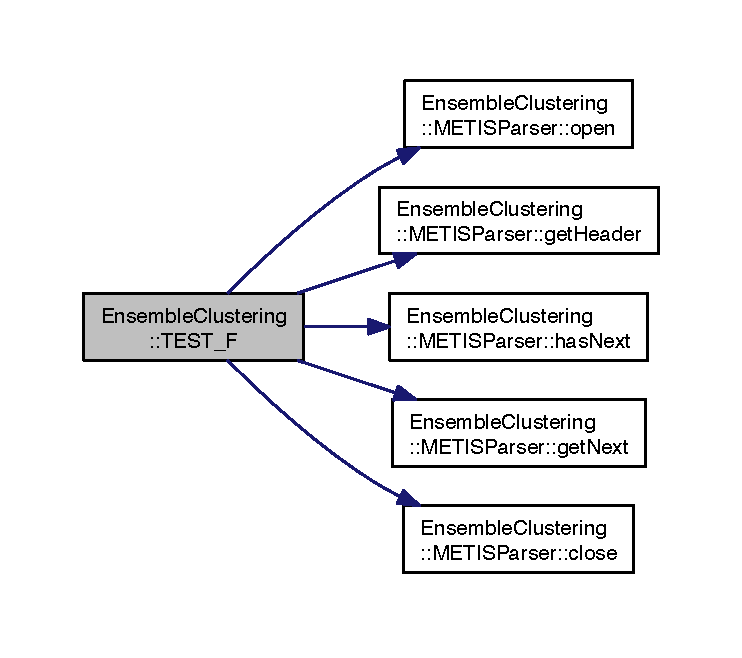
\includegraphics[width=350pt]{namespace_ensemble_clustering_a968aa929eb81f21fab68af5447226d50_cgraph}
\end{center}
\end{figure}


\hypertarget{namespace_ensemble_clustering_a21108087fb4225d2c718b2ab980a0352}{\index{Ensemble\-Clustering@{Ensemble\-Clustering}!T\-E\-S\-T\-\_\-\-F@{T\-E\-S\-T\-\_\-\-F}}
\index{T\-E\-S\-T\-\_\-\-F@{T\-E\-S\-T\-\_\-\-F}!EnsembleClustering@{Ensemble\-Clustering}}
\subsubsection[{T\-E\-S\-T\-\_\-\-F}]{\setlength{\rightskip}{0pt plus 5cm}Ensemble\-Clustering\-::\-T\-E\-S\-T\-\_\-\-F (
\begin{DoxyParamCaption}
\item[{Clustering\-Test}]{, }
\item[{test\-Modularity}]{}
\end{DoxyParamCaption}
)}}\label{namespace_ensemble_clustering_a21108087fb4225d2c718b2ab980a0352}


Definition at line 29 of file Clustering\-Test.\-h.



Here is the call graph for this function\-:
\nopagebreak
\begin{figure}[H]
\begin{center}
\leavevmode
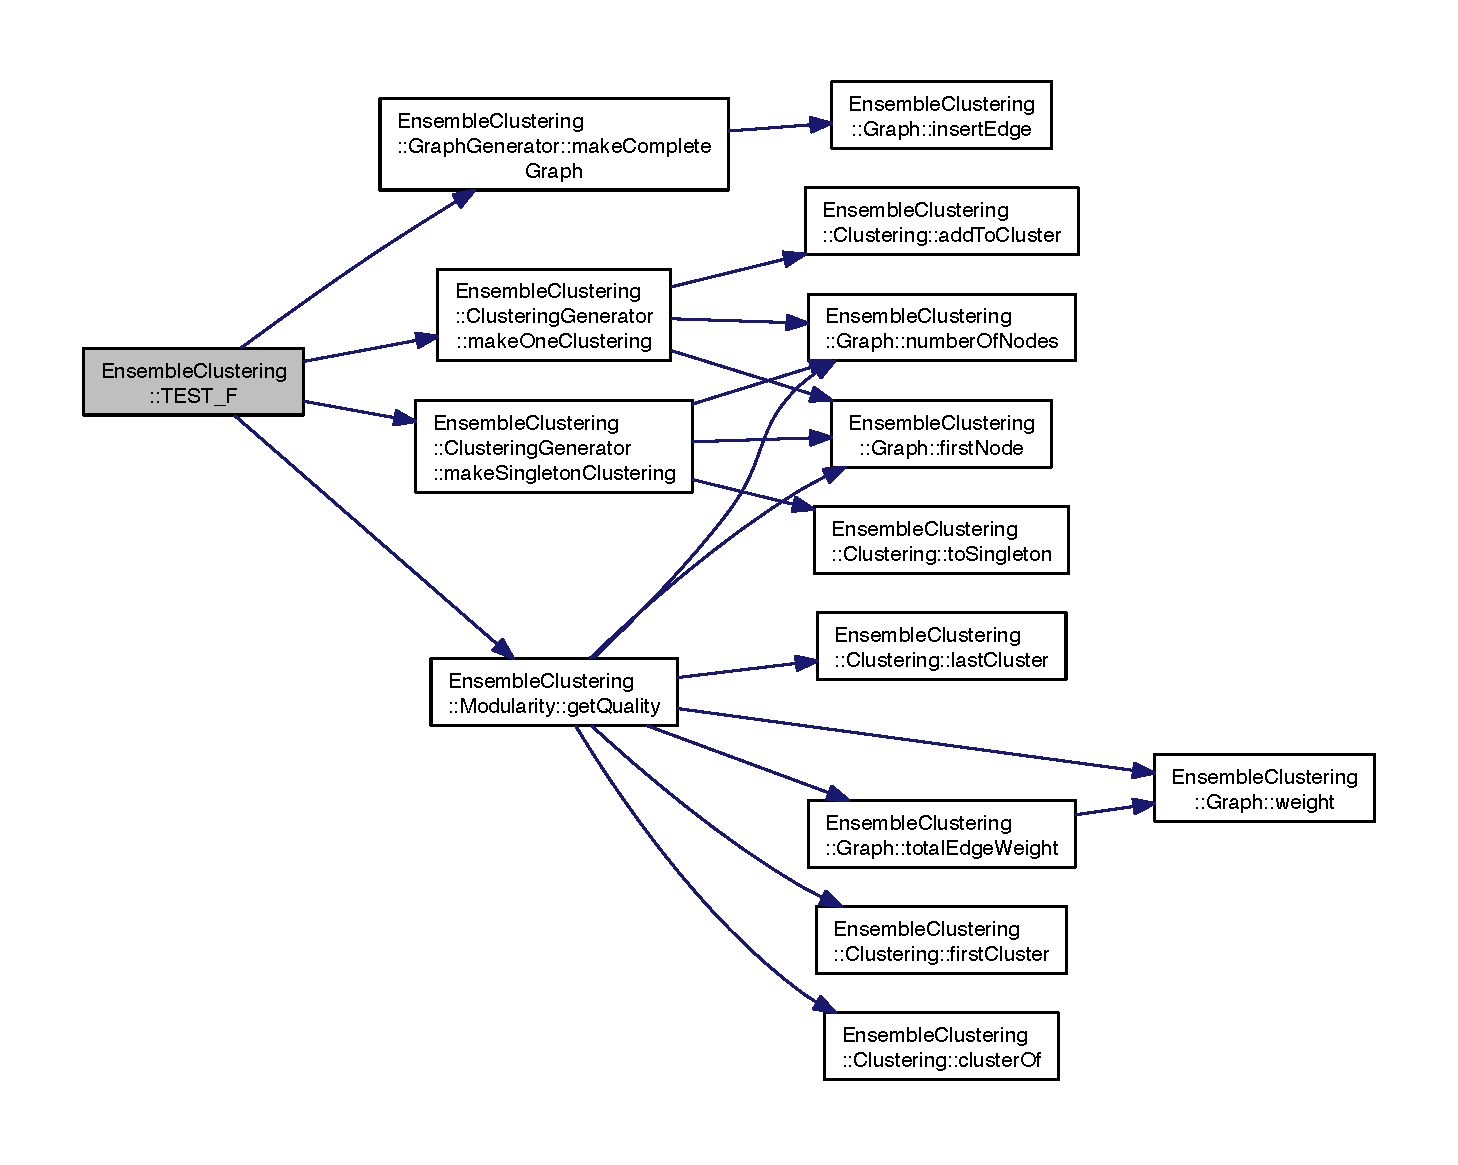
\includegraphics[width=350pt]{namespace_ensemble_clustering_a21108087fb4225d2c718b2ab980a0352_cgraph}
\end{center}
\end{figure}


\hypertarget{namespace_ensemble_clustering_ab112b02697a12bdbc3b4e866d60444d3}{\index{Ensemble\-Clustering@{Ensemble\-Clustering}!T\-E\-S\-T\-\_\-\-F@{T\-E\-S\-T\-\_\-\-F}}
\index{T\-E\-S\-T\-\_\-\-F@{T\-E\-S\-T\-\_\-\-F}!EnsembleClustering@{Ensemble\-Clustering}}
\subsubsection[{T\-E\-S\-T\-\_\-\-F}]{\setlength{\rightskip}{0pt plus 5cm}Ensemble\-Clustering\-::\-T\-E\-S\-T\-\_\-\-F (
\begin{DoxyParamCaption}
\item[{Graph\-G\-Test}]{, }
\item[{test\-Iteration}]{}
\end{DoxyParamCaption}
)}}\label{namespace_ensemble_clustering_ab112b02697a12bdbc3b4e866d60444d3}


Definition at line 34 of file Graph\-G\-Test.\-h.



Here is the call graph for this function\-:
\nopagebreak
\begin{figure}[H]
\begin{center}
\leavevmode
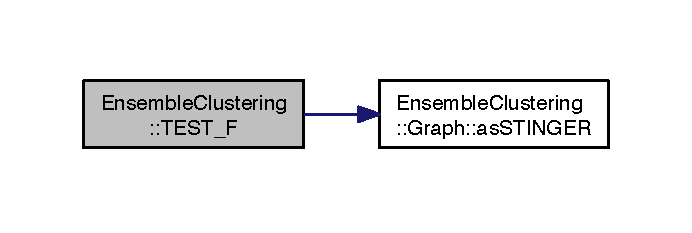
\includegraphics[width=332pt]{namespace_ensemble_clustering_ab112b02697a12bdbc3b4e866d60444d3_cgraph}
\end{center}
\end{figure}



\chapter{Class Documentation}
\hypertarget{class_ensemble_clustering_1_1_edge_scoring}{\section{Ensemble\-Clustering\-:\-:Edge\-Scoring Class Reference}
\label{class_ensemble_clustering_1_1_edge_scoring}\index{Ensemble\-Clustering\-::\-Edge\-Scoring@{Ensemble\-Clustering\-::\-Edge\-Scoring}}
}


{\ttfamily \#include $<$Edge\-Scoring.\-h$>$}



Inheritance diagram for Ensemble\-Clustering\-:\-:Edge\-Scoring\-:\nopagebreak
\begin{figure}[H]
\begin{center}
\leavevmode
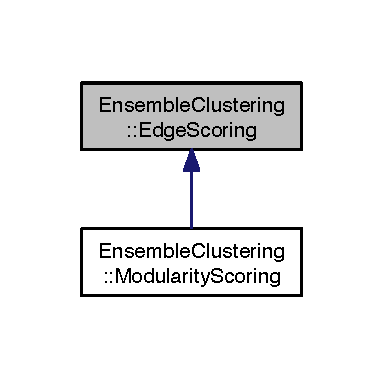
\includegraphics[width=184pt]{class_ensemble_clustering_1_1_edge_scoring__inherit__graph}
\end{center}
\end{figure}
\subsection*{Public Member Functions}
\begin{DoxyCompactItemize}
\item 
\hyperlink{class_ensemble_clustering_1_1_edge_scoring_a83339193ebf55255b09a34a2e1112eea}{Edge\-Scoring} ()
\item 
virtual \hyperlink{class_ensemble_clustering_1_1_edge_scoring_a1bb790ce6fd801ea40e0603785c73727}{$\sim$\-Edge\-Scoring} ()
\item 
virtual double \hyperlink{class_ensemble_clustering_1_1_edge_scoring_ae0b8ed83c76ea8f71f8246949d3106f4}{score\-Edge} (\hyperlink{namespace_ensemble_clustering_a136bcdc52fb2f62a89bc8bf8c1a7cb8f}{Node} u, \hyperlink{namespace_ensemble_clustering_a136bcdc52fb2f62a89bc8bf8c1a7cb8f}{Node} v)=0
\end{DoxyCompactItemize}


\subsection{Detailed Description}


Definition at line 16 of file Edge\-Scoring.\-h.



\subsection{Constructor \& Destructor Documentation}
\hypertarget{class_ensemble_clustering_1_1_edge_scoring_a83339193ebf55255b09a34a2e1112eea}{\index{Ensemble\-Clustering\-::\-Edge\-Scoring@{Ensemble\-Clustering\-::\-Edge\-Scoring}!Edge\-Scoring@{Edge\-Scoring}}
\index{Edge\-Scoring@{Edge\-Scoring}!EnsembleClustering::EdgeScoring@{Ensemble\-Clustering\-::\-Edge\-Scoring}}
\subsubsection[{Edge\-Scoring}]{\setlength{\rightskip}{0pt plus 5cm}Ensemble\-Clustering\-::\-Edge\-Scoring\-::\-Edge\-Scoring (
\begin{DoxyParamCaption}
{}
\end{DoxyParamCaption}
)}}\label{class_ensemble_clustering_1_1_edge_scoring_a83339193ebf55255b09a34a2e1112eea}


Definition at line 12 of file Edge\-Scoring.\-cpp.

\hypertarget{class_ensemble_clustering_1_1_edge_scoring_a1bb790ce6fd801ea40e0603785c73727}{\index{Ensemble\-Clustering\-::\-Edge\-Scoring@{Ensemble\-Clustering\-::\-Edge\-Scoring}!$\sim$\-Edge\-Scoring@{$\sim$\-Edge\-Scoring}}
\index{$\sim$\-Edge\-Scoring@{$\sim$\-Edge\-Scoring}!EnsembleClustering::EdgeScoring@{Ensemble\-Clustering\-::\-Edge\-Scoring}}
\subsubsection[{$\sim$\-Edge\-Scoring}]{\setlength{\rightskip}{0pt plus 5cm}Ensemble\-Clustering\-::\-Edge\-Scoring\-::$\sim$\-Edge\-Scoring (
\begin{DoxyParamCaption}
{}
\end{DoxyParamCaption}
)\hspace{0.3cm}{\ttfamily [virtual]}}}\label{class_ensemble_clustering_1_1_edge_scoring_a1bb790ce6fd801ea40e0603785c73727}


Definition at line 17 of file Edge\-Scoring.\-cpp.



\subsection{Member Function Documentation}
\hypertarget{class_ensemble_clustering_1_1_edge_scoring_ae0b8ed83c76ea8f71f8246949d3106f4}{\index{Ensemble\-Clustering\-::\-Edge\-Scoring@{Ensemble\-Clustering\-::\-Edge\-Scoring}!score\-Edge@{score\-Edge}}
\index{score\-Edge@{score\-Edge}!EnsembleClustering::EdgeScoring@{Ensemble\-Clustering\-::\-Edge\-Scoring}}
\subsubsection[{score\-Edge}]{\setlength{\rightskip}{0pt plus 5cm}virtual double Ensemble\-Clustering\-::\-Edge\-Scoring\-::score\-Edge (
\begin{DoxyParamCaption}
\item[{{\bf Node}}]{u, }
\item[{{\bf Node}}]{v}
\end{DoxyParamCaption}
)\hspace{0.3cm}{\ttfamily [pure virtual]}}}\label{class_ensemble_clustering_1_1_edge_scoring_ae0b8ed83c76ea8f71f8246949d3106f4}


The documentation for this class was generated from the following files\-:\begin{DoxyCompactItemize}
\item 
src/scoring/\hyperlink{_edge_scoring_8h}{Edge\-Scoring.\-h}\item 
src/scoring/\hyperlink{_edge_scoring_8cpp}{Edge\-Scoring.\-cpp}\end{DoxyCompactItemize}

\hypertarget{class_ensemble_clustering_1_1_edge_triple_graph_data}{\section{Ensemble\-Clustering\-:\-:Edge\-Triple\-Graph\-Data Class Reference}
\label{class_ensemble_clustering_1_1_edge_triple_graph_data}\index{Ensemble\-Clustering\-::\-Edge\-Triple\-Graph\-Data@{Ensemble\-Clustering\-::\-Edge\-Triple\-Graph\-Data}}
}


{\ttfamily \#include $<$Edge\-Triple\-Graph\-Data.\-h$>$}

\subsection*{Public Member Functions}
\begin{DoxyCompactItemize}
\item 
\hyperlink{class_ensemble_clustering_1_1_edge_triple_graph_data_a5bd6e67c6d4cfb6fcd3e93ad43b8d895}{Edge\-Triple\-Graph\-Data} (int \hyperlink{class_ensemble_clustering_1_1_edge_triple_graph_data_a907cee0110aa331fa3c3ddd99b8deaf7}{n}, int \hyperlink{class_ensemble_clustering_1_1_edge_triple_graph_data_a5ee6e7a60111a4120f880db9ae16d0cb}{m})
\item 
virtual \hyperlink{class_ensemble_clustering_1_1_edge_triple_graph_data_ac76298b736f2e358ca0212c9c1f0ec7b}{$\sim$\-Edge\-Triple\-Graph\-Data} ()
\end{DoxyCompactItemize}
\subsection*{Public Attributes}
\begin{DoxyCompactItemize}
\item 
int \hyperlink{class_ensemble_clustering_1_1_edge_triple_graph_data_a907cee0110aa331fa3c3ddd99b8deaf7}{n}
\begin{DoxyCompactList}\small\item\em number of nodes \end{DoxyCompactList}\item 
int \hyperlink{class_ensemble_clustering_1_1_edge_triple_graph_data_a5ee6e7a60111a4120f880db9ae16d0cb}{m}
\begin{DoxyCompactList}\small\item\em number of edges \end{DoxyCompactList}\item 
\hyperlink{class_ensemble_clustering_1_1_edge_tuple}{Edge\-Tuple} $\ast$ \hyperlink{class_ensemble_clustering_1_1_edge_triple_graph_data_acb27bbd92c258f29537e2d9a94e973ea}{edge\-Data}
\item 
\hyperlink{class_ensemble_clustering_1_1_node_tuple}{Node\-Tuple} $\ast$ \hyperlink{class_ensemble_clustering_1_1_edge_triple_graph_data_ac9d42d7b576078953b3ddbae01004dd8}{node\-Data}
\end{DoxyCompactItemize}


\subsection{Detailed Description}


Definition at line 50 of file Edge\-Triple\-Graph\-Data.\-h.



\subsection{Constructor \& Destructor Documentation}
\hypertarget{class_ensemble_clustering_1_1_edge_triple_graph_data_a5bd6e67c6d4cfb6fcd3e93ad43b8d895}{\index{Ensemble\-Clustering\-::\-Edge\-Triple\-Graph\-Data@{Ensemble\-Clustering\-::\-Edge\-Triple\-Graph\-Data}!Edge\-Triple\-Graph\-Data@{Edge\-Triple\-Graph\-Data}}
\index{Edge\-Triple\-Graph\-Data@{Edge\-Triple\-Graph\-Data}!EnsembleClustering::EdgeTripleGraphData@{Ensemble\-Clustering\-::\-Edge\-Triple\-Graph\-Data}}
\subsubsection[{Edge\-Triple\-Graph\-Data}]{\setlength{\rightskip}{0pt plus 5cm}Ensemble\-Clustering\-::\-Edge\-Triple\-Graph\-Data\-::\-Edge\-Triple\-Graph\-Data (
\begin{DoxyParamCaption}
\item[{int}]{n, }
\item[{int}]{m}
\end{DoxyParamCaption}
)}}\label{class_ensemble_clustering_1_1_edge_triple_graph_data_a5bd6e67c6d4cfb6fcd3e93ad43b8d895}


Definition at line 37 of file Edge\-Triple\-Graph\-Data.\-cpp.

\hypertarget{class_ensemble_clustering_1_1_edge_triple_graph_data_ac76298b736f2e358ca0212c9c1f0ec7b}{\index{Ensemble\-Clustering\-::\-Edge\-Triple\-Graph\-Data@{Ensemble\-Clustering\-::\-Edge\-Triple\-Graph\-Data}!$\sim$\-Edge\-Triple\-Graph\-Data@{$\sim$\-Edge\-Triple\-Graph\-Data}}
\index{$\sim$\-Edge\-Triple\-Graph\-Data@{$\sim$\-Edge\-Triple\-Graph\-Data}!EnsembleClustering::EdgeTripleGraphData@{Ensemble\-Clustering\-::\-Edge\-Triple\-Graph\-Data}}
\subsubsection[{$\sim$\-Edge\-Triple\-Graph\-Data}]{\setlength{\rightskip}{0pt plus 5cm}Ensemble\-Clustering\-::\-Edge\-Triple\-Graph\-Data\-::$\sim$\-Edge\-Triple\-Graph\-Data (
\begin{DoxyParamCaption}
{}
\end{DoxyParamCaption}
)\hspace{0.3cm}{\ttfamily [virtual]}}}\label{class_ensemble_clustering_1_1_edge_triple_graph_data_ac76298b736f2e358ca0212c9c1f0ec7b}


Definition at line 46 of file Edge\-Triple\-Graph\-Data.\-cpp.



\subsection{Member Data Documentation}
\hypertarget{class_ensemble_clustering_1_1_edge_triple_graph_data_acb27bbd92c258f29537e2d9a94e973ea}{\index{Ensemble\-Clustering\-::\-Edge\-Triple\-Graph\-Data@{Ensemble\-Clustering\-::\-Edge\-Triple\-Graph\-Data}!edge\-Data@{edge\-Data}}
\index{edge\-Data@{edge\-Data}!EnsembleClustering::EdgeTripleGraphData@{Ensemble\-Clustering\-::\-Edge\-Triple\-Graph\-Data}}
\subsubsection[{edge\-Data}]{\setlength{\rightskip}{0pt plus 5cm}{\bf Edge\-Tuple}$\ast$ Ensemble\-Clustering\-::\-Edge\-Triple\-Graph\-Data\-::edge\-Data}}\label{class_ensemble_clustering_1_1_edge_triple_graph_data_acb27bbd92c258f29537e2d9a94e973ea}


Definition at line 61 of file Edge\-Triple\-Graph\-Data.\-h.

\hypertarget{class_ensemble_clustering_1_1_edge_triple_graph_data_a5ee6e7a60111a4120f880db9ae16d0cb}{\index{Ensemble\-Clustering\-::\-Edge\-Triple\-Graph\-Data@{Ensemble\-Clustering\-::\-Edge\-Triple\-Graph\-Data}!m@{m}}
\index{m@{m}!EnsembleClustering::EdgeTripleGraphData@{Ensemble\-Clustering\-::\-Edge\-Triple\-Graph\-Data}}
\subsubsection[{m}]{\setlength{\rightskip}{0pt plus 5cm}int Ensemble\-Clustering\-::\-Edge\-Triple\-Graph\-Data\-::m}}\label{class_ensemble_clustering_1_1_edge_triple_graph_data_a5ee6e7a60111a4120f880db9ae16d0cb}


number of edges 



Definition at line 59 of file Edge\-Triple\-Graph\-Data.\-h.

\hypertarget{class_ensemble_clustering_1_1_edge_triple_graph_data_a907cee0110aa331fa3c3ddd99b8deaf7}{\index{Ensemble\-Clustering\-::\-Edge\-Triple\-Graph\-Data@{Ensemble\-Clustering\-::\-Edge\-Triple\-Graph\-Data}!n@{n}}
\index{n@{n}!EnsembleClustering::EdgeTripleGraphData@{Ensemble\-Clustering\-::\-Edge\-Triple\-Graph\-Data}}
\subsubsection[{n}]{\setlength{\rightskip}{0pt plus 5cm}int Ensemble\-Clustering\-::\-Edge\-Triple\-Graph\-Data\-::n}}\label{class_ensemble_clustering_1_1_edge_triple_graph_data_a907cee0110aa331fa3c3ddd99b8deaf7}


number of nodes 



Definition at line 58 of file Edge\-Triple\-Graph\-Data.\-h.

\hypertarget{class_ensemble_clustering_1_1_edge_triple_graph_data_ac9d42d7b576078953b3ddbae01004dd8}{\index{Ensemble\-Clustering\-::\-Edge\-Triple\-Graph\-Data@{Ensemble\-Clustering\-::\-Edge\-Triple\-Graph\-Data}!node\-Data@{node\-Data}}
\index{node\-Data@{node\-Data}!EnsembleClustering::EdgeTripleGraphData@{Ensemble\-Clustering\-::\-Edge\-Triple\-Graph\-Data}}
\subsubsection[{node\-Data}]{\setlength{\rightskip}{0pt plus 5cm}{\bf Node\-Tuple}$\ast$ Ensemble\-Clustering\-::\-Edge\-Triple\-Graph\-Data\-::node\-Data}}\label{class_ensemble_clustering_1_1_edge_triple_graph_data_ac9d42d7b576078953b3ddbae01004dd8}


Definition at line 62 of file Edge\-Triple\-Graph\-Data.\-h.



The documentation for this class was generated from the following files\-:\begin{DoxyCompactItemize}
\item 
src/\hyperlink{_edge_triple_graph_data_8h}{Edge\-Triple\-Graph\-Data.\-h}\item 
src/\hyperlink{_edge_triple_graph_data_8cpp}{Edge\-Triple\-Graph\-Data.\-cpp}\end{DoxyCompactItemize}

\hypertarget{class_ensemble_clustering_1_1_edge_tuple}{\section{Ensemble\-Clustering\-:\-:Edge\-Tuple Class Reference}
\label{class_ensemble_clustering_1_1_edge_tuple}\index{Ensemble\-Clustering\-::\-Edge\-Tuple@{Ensemble\-Clustering\-::\-Edge\-Tuple}}
}


\hyperlink{class_ensemble_clustering_1_1_edge_tuple}{Edge\-Tuple} contains triple (i, j, w) where i\-: edge source index j\-: edge target index w\-: edge weight.  




{\ttfamily \#include $<$Edge\-Triple\-Graph\-Data.\-h$>$}

\subsection*{Public Member Functions}
\begin{DoxyCompactItemize}
\item 
\hyperlink{class_ensemble_clustering_1_1_edge_tuple_a5d6d569201ed9d751992e9fa85cb668a}{Edge\-Tuple} ()
\item 
\hyperlink{class_ensemble_clustering_1_1_edge_tuple_a70a0783ed608657fe6c64c87f783be83}{Edge\-Tuple} (int \hyperlink{class_ensemble_clustering_1_1_edge_tuple_acf12140619e42d9e60ccf402caf0730d}{i}, int \hyperlink{class_ensemble_clustering_1_1_edge_tuple_a8f3e5de46a3c3e1eefeda14d6330eaab}{j}, double \hyperlink{class_ensemble_clustering_1_1_edge_tuple_a5dbd8079be78b2057d441f79eae7c905}{w})
\end{DoxyCompactItemize}
\subsection*{Public Attributes}
\begin{DoxyCompactItemize}
\item 
int \hyperlink{class_ensemble_clustering_1_1_edge_tuple_acf12140619e42d9e60ccf402caf0730d}{i}
\begin{DoxyCompactList}\small\item\em edge source index \end{DoxyCompactList}\item 
int \hyperlink{class_ensemble_clustering_1_1_edge_tuple_a8f3e5de46a3c3e1eefeda14d6330eaab}{j}
\begin{DoxyCompactList}\small\item\em edge target index \end{DoxyCompactList}\item 
double \hyperlink{class_ensemble_clustering_1_1_edge_tuple_a5dbd8079be78b2057d441f79eae7c905}{w}
\begin{DoxyCompactList}\small\item\em edge weight \end{DoxyCompactList}\end{DoxyCompactItemize}


\subsection{Detailed Description}
\hyperlink{class_ensemble_clustering_1_1_edge_tuple}{Edge\-Tuple} contains triple (i, j, w) where i\-: edge source index j\-: edge target index w\-: edge weight. 

Definition at line 21 of file Edge\-Triple\-Graph\-Data.\-h.



\subsection{Constructor \& Destructor Documentation}
\hypertarget{class_ensemble_clustering_1_1_edge_tuple_a5d6d569201ed9d751992e9fa85cb668a}{\index{Ensemble\-Clustering\-::\-Edge\-Tuple@{Ensemble\-Clustering\-::\-Edge\-Tuple}!Edge\-Tuple@{Edge\-Tuple}}
\index{Edge\-Tuple@{Edge\-Tuple}!EnsembleClustering::EdgeTuple@{Ensemble\-Clustering\-::\-Edge\-Tuple}}
\subsubsection[{Edge\-Tuple}]{\setlength{\rightskip}{0pt plus 5cm}Ensemble\-Clustering\-::\-Edge\-Tuple\-::\-Edge\-Tuple (
\begin{DoxyParamCaption}
{}
\end{DoxyParamCaption}
)}}\label{class_ensemble_clustering_1_1_edge_tuple_a5d6d569201ed9d751992e9fa85cb668a}


Definition at line 13 of file Edge\-Triple\-Graph\-Data.\-cpp.

\hypertarget{class_ensemble_clustering_1_1_edge_tuple_a70a0783ed608657fe6c64c87f783be83}{\index{Ensemble\-Clustering\-::\-Edge\-Tuple@{Ensemble\-Clustering\-::\-Edge\-Tuple}!Edge\-Tuple@{Edge\-Tuple}}
\index{Edge\-Tuple@{Edge\-Tuple}!EnsembleClustering::EdgeTuple@{Ensemble\-Clustering\-::\-Edge\-Tuple}}
\subsubsection[{Edge\-Tuple}]{\setlength{\rightskip}{0pt plus 5cm}Ensemble\-Clustering\-::\-Edge\-Tuple\-::\-Edge\-Tuple (
\begin{DoxyParamCaption}
\item[{int}]{i, }
\item[{int}]{j, }
\item[{double}]{w}
\end{DoxyParamCaption}
)}}\label{class_ensemble_clustering_1_1_edge_tuple_a70a0783ed608657fe6c64c87f783be83}


Definition at line 19 of file Edge\-Triple\-Graph\-Data.\-cpp.



\subsection{Member Data Documentation}
\hypertarget{class_ensemble_clustering_1_1_edge_tuple_acf12140619e42d9e60ccf402caf0730d}{\index{Ensemble\-Clustering\-::\-Edge\-Tuple@{Ensemble\-Clustering\-::\-Edge\-Tuple}!i@{i}}
\index{i@{i}!EnsembleClustering::EdgeTuple@{Ensemble\-Clustering\-::\-Edge\-Tuple}}
\subsubsection[{i}]{\setlength{\rightskip}{0pt plus 5cm}int Ensemble\-Clustering\-::\-Edge\-Tuple\-::i}}\label{class_ensemble_clustering_1_1_edge_tuple_acf12140619e42d9e60ccf402caf0730d}


edge source index 



Definition at line 29 of file Edge\-Triple\-Graph\-Data.\-h.

\hypertarget{class_ensemble_clustering_1_1_edge_tuple_a8f3e5de46a3c3e1eefeda14d6330eaab}{\index{Ensemble\-Clustering\-::\-Edge\-Tuple@{Ensemble\-Clustering\-::\-Edge\-Tuple}!j@{j}}
\index{j@{j}!EnsembleClustering::EdgeTuple@{Ensemble\-Clustering\-::\-Edge\-Tuple}}
\subsubsection[{j}]{\setlength{\rightskip}{0pt plus 5cm}int Ensemble\-Clustering\-::\-Edge\-Tuple\-::j}}\label{class_ensemble_clustering_1_1_edge_tuple_a8f3e5de46a3c3e1eefeda14d6330eaab}


edge target index 



Definition at line 30 of file Edge\-Triple\-Graph\-Data.\-h.

\hypertarget{class_ensemble_clustering_1_1_edge_tuple_a5dbd8079be78b2057d441f79eae7c905}{\index{Ensemble\-Clustering\-::\-Edge\-Tuple@{Ensemble\-Clustering\-::\-Edge\-Tuple}!w@{w}}
\index{w@{w}!EnsembleClustering::EdgeTuple@{Ensemble\-Clustering\-::\-Edge\-Tuple}}
\subsubsection[{w}]{\setlength{\rightskip}{0pt plus 5cm}double Ensemble\-Clustering\-::\-Edge\-Tuple\-::w}}\label{class_ensemble_clustering_1_1_edge_tuple_a5dbd8079be78b2057d441f79eae7c905}


edge weight 



Definition at line 31 of file Edge\-Triple\-Graph\-Data.\-h.



The documentation for this class was generated from the following files\-:\begin{DoxyCompactItemize}
\item 
src/\hyperlink{_edge_triple_graph_data_8h}{Edge\-Triple\-Graph\-Data.\-h}\item 
src/\hyperlink{_edge_triple_graph_data_8cpp}{Edge\-Triple\-Graph\-Data.\-cpp}\end{DoxyCompactItemize}

\hypertarget{class_ensemble_clustering_1_1_ensemble_clustering_algo}{\section{Ensemble\-Clustering\-:\-:Ensemble\-Clustering\-Algo Class Reference}
\label{class_ensemble_clustering_1_1_ensemble_clustering_algo}\index{Ensemble\-Clustering\-::\-Ensemble\-Clustering\-Algo@{Ensemble\-Clustering\-::\-Ensemble\-Clustering\-Algo}}
}


{\ttfamily \#include $<$Ensemble\-Clustering\-Algo.\-h$>$}

\subsection*{Public Member Functions}
\begin{DoxyCompactItemize}
\item 
\hyperlink{class_ensemble_clustering_1_1_ensemble_clustering_algo_aafaaa6db31675b8127ed0de3e3499c7b}{Ensemble\-Clustering\-Algo} ()
\item 
virtual \hyperlink{class_ensemble_clustering_1_1_ensemble_clustering_algo_a213c23187f025f36f32df455b4c2958f}{$\sim$\-Ensemble\-Clustering\-Algo} ()
\end{DoxyCompactItemize}


\subsection{Detailed Description}


Definition at line 13 of file Ensemble\-Clustering\-Algo.\-h.



\subsection{Constructor \& Destructor Documentation}
\hypertarget{class_ensemble_clustering_1_1_ensemble_clustering_algo_aafaaa6db31675b8127ed0de3e3499c7b}{\index{Ensemble\-Clustering\-::\-Ensemble\-Clustering\-Algo@{Ensemble\-Clustering\-::\-Ensemble\-Clustering\-Algo}!Ensemble\-Clustering\-Algo@{Ensemble\-Clustering\-Algo}}
\index{Ensemble\-Clustering\-Algo@{Ensemble\-Clustering\-Algo}!EnsembleClustering::EnsembleClusteringAlgo@{Ensemble\-Clustering\-::\-Ensemble\-Clustering\-Algo}}
\subsubsection[{Ensemble\-Clustering\-Algo}]{\setlength{\rightskip}{0pt plus 5cm}Ensemble\-Clustering\-::\-Ensemble\-Clustering\-Algo\-::\-Ensemble\-Clustering\-Algo (
\begin{DoxyParamCaption}
{}
\end{DoxyParamCaption}
)}}\label{class_ensemble_clustering_1_1_ensemble_clustering_algo_aafaaa6db31675b8127ed0de3e3499c7b}


Definition at line 12 of file Ensemble\-Clustering\-Algo.\-cpp.

\hypertarget{class_ensemble_clustering_1_1_ensemble_clustering_algo_a213c23187f025f36f32df455b4c2958f}{\index{Ensemble\-Clustering\-::\-Ensemble\-Clustering\-Algo@{Ensemble\-Clustering\-::\-Ensemble\-Clustering\-Algo}!$\sim$\-Ensemble\-Clustering\-Algo@{$\sim$\-Ensemble\-Clustering\-Algo}}
\index{$\sim$\-Ensemble\-Clustering\-Algo@{$\sim$\-Ensemble\-Clustering\-Algo}!EnsembleClustering::EnsembleClusteringAlgo@{Ensemble\-Clustering\-::\-Ensemble\-Clustering\-Algo}}
\subsubsection[{$\sim$\-Ensemble\-Clustering\-Algo}]{\setlength{\rightskip}{0pt plus 5cm}Ensemble\-Clustering\-::\-Ensemble\-Clustering\-Algo\-::$\sim$\-Ensemble\-Clustering\-Algo (
\begin{DoxyParamCaption}
{}
\end{DoxyParamCaption}
)\hspace{0.3cm}{\ttfamily [virtual]}}}\label{class_ensemble_clustering_1_1_ensemble_clustering_algo_a213c23187f025f36f32df455b4c2958f}


Definition at line 17 of file Ensemble\-Clustering\-Algo.\-cpp.



The documentation for this class was generated from the following files\-:\begin{DoxyCompactItemize}
\item 
src/\hyperlink{_ensemble_clustering_algo_8h}{Ensemble\-Clustering\-Algo.\-h}\item 
src/\hyperlink{_ensemble_clustering_algo_8cpp}{Ensemble\-Clustering\-Algo.\-cpp}\end{DoxyCompactItemize}

\hypertarget{class_ensemble_clustering_1_1_graph}{\section{Ensemble\-Clustering\-:\-:Graph Class Reference}
\label{class_ensemble_clustering_1_1_graph}\index{Ensemble\-Clustering\-::\-Graph@{Ensemble\-Clustering\-::\-Graph}}
}


\hyperlink{class_ensemble_clustering_1_1_graph}{Graph} interface.  




{\ttfamily \#include $<$Graph.\-h$>$}

\subsection*{Public Member Functions}
\begin{DoxyCompactItemize}
\item 
\hyperlink{class_ensemble_clustering_1_1_graph_a65031e76ae95333341f795fb9a13647f}{Graph} ()
\begin{DoxyCompactList}\small\item\em methods \end{DoxyCompactList}\item 
\hyperlink{class_ensemble_clustering_1_1_graph_a0ffcdfea431e8c85de2058a226a4783a}{Graph} (stinger $\ast$\hyperlink{class_ensemble_clustering_1_1_graph_af83709e85afb91c70729405a725afb9a}{stinger\-G})
\begin{DoxyCompactList}\small\item\em Initialize with S\-T\-I\-N\-G\-E\-R graph. \end{DoxyCompactList}\item 
\hyperlink{class_ensemble_clustering_1_1_graph_ac8368ff972ce067d51e37c48124a0038}{$\sim$\-Graph} ()
\item 
stinger $\ast$ \hyperlink{class_ensemble_clustering_1_1_graph_ad7ad5a71649990fe2b823b8ed7a113b7}{as\-S\-T\-I\-N\-G\-E\-R} () const 
\begin{DoxyCompactList}\small\item\em Return the internal S\-T\-I\-N\-G\-E\-R data structure. \end{DoxyCompactList}\item 
void \hyperlink{class_ensemble_clustering_1_1_graph_a78d527f03a3a860ee173dadbaefe1d5c}{insert\-Edge} (\hyperlink{namespace_ensemble_clustering_ae829290aeccd1a420b17a37fd901f114}{node} u, \hyperlink{namespace_ensemble_clustering_ae829290aeccd1a420b17a37fd901f114}{node} v, double \hyperlink{class_ensemble_clustering_1_1_graph_a9bff231567f9ac604f1854d62f6682d1}{weight}=\hyperlink{class_ensemble_clustering_1_1_graph_a8186ee969064a4e12b779b1dc506ac60}{default\-Edge\-Weight}, int64\-\_\-t type=\hyperlink{class_ensemble_clustering_1_1_graph_a377621f37c1dc58f32ecec0fd229408e}{default\-Edge\-Type}, int64\-\_\-t timestamp=\hyperlink{class_ensemble_clustering_1_1_graph_a9a6623d55f673a3b30e0c23284dd6da1}{default\-Time\-Stamp})
\begin{DoxyCompactList}\small\item\em Insert a weighted, undirected edge. \end{DoxyCompactList}\item 
bool \hyperlink{class_ensemble_clustering_1_1_graph_a9be0c0a70204723e4b040b9cba51b15d}{has\-Edge} (\hyperlink{namespace_ensemble_clustering_ae829290aeccd1a420b17a37fd901f114}{node} u, \hyperlink{namespace_ensemble_clustering_ae829290aeccd1a420b17a37fd901f114}{node} v) const 
\begin{DoxyCompactList}\small\item\em Check if undirected edge \{u,v\} exists in G. \end{DoxyCompactList}\item 
double \hyperlink{class_ensemble_clustering_1_1_graph_a9bff231567f9ac604f1854d62f6682d1}{weight} (\hyperlink{namespace_ensemble_clustering_ae829290aeccd1a420b17a37fd901f114}{node} v) const 
\begin{DoxyCompactList}\small\item\em Return node weight. \end{DoxyCompactList}\item 
double \hyperlink{class_ensemble_clustering_1_1_graph_a656f5cb3119dd3f8f4182d38cce82fa0}{weight} (\hyperlink{namespace_ensemble_clustering_aff19dd5e3051ee3d4360fd3f29daf16b}{edge} uv) const 
\begin{DoxyCompactList}\small\item\em Return edge weight. \end{DoxyCompactList}\item 
double \hyperlink{class_ensemble_clustering_1_1_graph_a4699131f4d3602ecda00eaf70a86cbea}{weight} (\hyperlink{namespace_ensemble_clustering_ae829290aeccd1a420b17a37fd901f114}{node} u, \hyperlink{namespace_ensemble_clustering_ae829290aeccd1a420b17a37fd901f114}{node} v) const 
\begin{DoxyCompactList}\small\item\em Return edge weight. \end{DoxyCompactList}\item 
double \hyperlink{class_ensemble_clustering_1_1_graph_a7be7f13f5a31b0513293e7bbac26ca6c}{total\-Edge\-Weight} () const 
\begin{DoxyCompactList}\small\item\em Get the sum of the weight of all edges. \end{DoxyCompactList}\item 
int64\-\_\-t \hyperlink{class_ensemble_clustering_1_1_graph_a35f4b169cd0157117b468b1863a0d70a}{degree} (\hyperlink{namespace_ensemble_clustering_ae829290aeccd1a420b17a37fd901f114}{node} u) const 
\begin{DoxyCompactList}\small\item\em Return the degree (number of incident edges). \end{DoxyCompactList}\item 
int64\-\_\-t \hyperlink{class_ensemble_clustering_1_1_graph_ab019840b239c3247eaf00e5ffcc6bb03}{number\-Of\-Edges} () const 
\begin{DoxyCompactList}\small\item\em Return the number of edges in the graph. \end{DoxyCompactList}\item 
int64\-\_\-t \hyperlink{class_ensemble_clustering_1_1_graph_affe61a24e54266aba872272fb9501c61}{number\-Of\-Nodes} () const 
\begin{DoxyCompactList}\small\item\em Return the number of (non-\/isolated) nodes in the graph. \end{DoxyCompactList}\item 
\hyperlink{namespace_ensemble_clustering_ae829290aeccd1a420b17a37fd901f114}{node} \hyperlink{class_ensemble_clustering_1_1_graph_aaac8bcc5d64461cba54ad38ec929be3c}{first\-Node} () const 
\begin{DoxyCompactList}\small\item\em Get the first node index (for iteration over all nodes) \end{DoxyCompactList}\item 
\hyperlink{namespace_ensemble_clustering_ae829290aeccd1a420b17a37fd901f114}{node} \hyperlink{class_ensemble_clustering_1_1_graph_a3d6fe2d0c27605f4b55585198eb9b933}{last\-Node} () const 
\begin{DoxyCompactList}\small\item\em Get the last node index (for iteration over all nodes). \end{DoxyCompactList}\item 
{\footnotesize template$<$typename Callback $>$ }\\void \hyperlink{class_ensemble_clustering_1_1_graph_a7b599771f8dc476712ea7e6b52157a3f}{forall\-Edges} (bool parallel, Callback callback)
\end{DoxyCompactItemize}
\subsection*{Static Public Attributes}
\begin{DoxyCompactItemize}
\item 
static constexpr double \hyperlink{class_ensemble_clustering_1_1_graph_a8186ee969064a4e12b779b1dc506ac60}{default\-Edge\-Weight} = 1.\-0
\begin{DoxyCompactList}\small\item\em default parameters \end{DoxyCompactList}\item 
static const int64\-\_\-t \hyperlink{class_ensemble_clustering_1_1_graph_a377621f37c1dc58f32ecec0fd229408e}{default\-Edge\-Type} = 0
\item 
static const int64\-\_\-t \hyperlink{class_ensemble_clustering_1_1_graph_a9a6623d55f673a3b30e0c23284dd6da1}{default\-Time\-Stamp} = 0
\end{DoxyCompactItemize}
\subsection*{Protected Attributes}
\begin{DoxyCompactItemize}
\item 
stinger $\ast$ \hyperlink{class_ensemble_clustering_1_1_graph_af83709e85afb91c70729405a725afb9a}{stinger\-G}
\end{DoxyCompactItemize}


\subsection{Detailed Description}
\hyperlink{class_ensemble_clustering_1_1_graph}{Graph} interface. 

\hyperlink{class_ensemble_clustering_1_1_graph}{Graph} encapsulates a S\-T\-I\-N\-G\-E\-R graph object and provides a more concise interface to it.

The graph concept modelled is
\begin{DoxyItemize}
\item undirected
\item weighted
\item without self-\/loops (use node weights instead) 
\end{DoxyItemize}

Definition at line 77 of file Graph.\-h.



\subsection{Constructor \& Destructor Documentation}
\hypertarget{class_ensemble_clustering_1_1_graph_a65031e76ae95333341f795fb9a13647f}{\index{Ensemble\-Clustering\-::\-Graph@{Ensemble\-Clustering\-::\-Graph}!Graph@{Graph}}
\index{Graph@{Graph}!EnsembleClustering::Graph@{Ensemble\-Clustering\-::\-Graph}}
\subsubsection[{Graph}]{\setlength{\rightskip}{0pt plus 5cm}Ensemble\-Clustering\-::\-Graph\-::\-Graph (
\begin{DoxyParamCaption}
{}
\end{DoxyParamCaption}
)}}\label{class_ensemble_clustering_1_1_graph_a65031e76ae95333341f795fb9a13647f}


methods 

Construct \hyperlink{class_ensemble_clustering_1_1_graph}{Graph} object with new S\-T\-I\-N\-G\-E\-R graph inside. 

Definition at line 13 of file Graph.\-cpp.

\hypertarget{class_ensemble_clustering_1_1_graph_a0ffcdfea431e8c85de2058a226a4783a}{\index{Ensemble\-Clustering\-::\-Graph@{Ensemble\-Clustering\-::\-Graph}!Graph@{Graph}}
\index{Graph@{Graph}!EnsembleClustering::Graph@{Ensemble\-Clustering\-::\-Graph}}
\subsubsection[{Graph}]{\setlength{\rightskip}{0pt plus 5cm}Ensemble\-Clustering\-::\-Graph\-::\-Graph (
\begin{DoxyParamCaption}
\item[{stinger $\ast$}]{stinger\-G}
\end{DoxyParamCaption}
)}}\label{class_ensemble_clustering_1_1_graph_a0ffcdfea431e8c85de2058a226a4783a}


Initialize with S\-T\-I\-N\-G\-E\-R graph. 


\begin{DoxyParams}[1]{Parameters}
\mbox{\tt in}  & {\em stinger\-G} & a S\-T\-I\-N\-G\-E\-R graph struct \\
\hline
\end{DoxyParams}


Definition at line 20 of file Graph.\-cpp.

\hypertarget{class_ensemble_clustering_1_1_graph_ac8368ff972ce067d51e37c48124a0038}{\index{Ensemble\-Clustering\-::\-Graph@{Ensemble\-Clustering\-::\-Graph}!$\sim$\-Graph@{$\sim$\-Graph}}
\index{$\sim$\-Graph@{$\sim$\-Graph}!EnsembleClustering::Graph@{Ensemble\-Clustering\-::\-Graph}}
\subsubsection[{$\sim$\-Graph}]{\setlength{\rightskip}{0pt plus 5cm}Ensemble\-Clustering\-::\-Graph\-::$\sim$\-Graph (
\begin{DoxyParamCaption}
{}
\end{DoxyParamCaption}
)}}\label{class_ensemble_clustering_1_1_graph_ac8368ff972ce067d51e37c48124a0038}


Definition at line 17 of file Graph.\-cpp.



\subsection{Member Function Documentation}
\hypertarget{class_ensemble_clustering_1_1_graph_ad7ad5a71649990fe2b823b8ed7a113b7}{\index{Ensemble\-Clustering\-::\-Graph@{Ensemble\-Clustering\-::\-Graph}!as\-S\-T\-I\-N\-G\-E\-R@{as\-S\-T\-I\-N\-G\-E\-R}}
\index{as\-S\-T\-I\-N\-G\-E\-R@{as\-S\-T\-I\-N\-G\-E\-R}!EnsembleClustering::Graph@{Ensemble\-Clustering\-::\-Graph}}
\subsubsection[{as\-S\-T\-I\-N\-G\-E\-R}]{\setlength{\rightskip}{0pt plus 5cm}stinger $\ast$ Ensemble\-Clustering\-::\-Graph\-::as\-S\-T\-I\-N\-G\-E\-R (
\begin{DoxyParamCaption}
{}
\end{DoxyParamCaption}
) const}}\label{class_ensemble_clustering_1_1_graph_ad7ad5a71649990fe2b823b8ed7a113b7}


Return the internal S\-T\-I\-N\-G\-E\-R data structure. 



Definition at line 26 of file Graph.\-cpp.

\hypertarget{class_ensemble_clustering_1_1_graph_a35f4b169cd0157117b468b1863a0d70a}{\index{Ensemble\-Clustering\-::\-Graph@{Ensemble\-Clustering\-::\-Graph}!degree@{degree}}
\index{degree@{degree}!EnsembleClustering::Graph@{Ensemble\-Clustering\-::\-Graph}}
\subsubsection[{degree}]{\setlength{\rightskip}{0pt plus 5cm}int64\-\_\-t Ensemble\-Clustering\-::\-Graph\-::degree (
\begin{DoxyParamCaption}
\item[{{\bf node}}]{u}
\end{DoxyParamCaption}
) const}}\label{class_ensemble_clustering_1_1_graph_a35f4b169cd0157117b468b1863a0d70a}


Return the degree (number of incident edges). 



Definition at line 69 of file Graph.\-cpp.

\hypertarget{class_ensemble_clustering_1_1_graph_aaac8bcc5d64461cba54ad38ec929be3c}{\index{Ensemble\-Clustering\-::\-Graph@{Ensemble\-Clustering\-::\-Graph}!first\-Node@{first\-Node}}
\index{first\-Node@{first\-Node}!EnsembleClustering::Graph@{Ensemble\-Clustering\-::\-Graph}}
\subsubsection[{first\-Node}]{\setlength{\rightskip}{0pt plus 5cm}{\bf node} Ensemble\-Clustering\-::\-Graph\-::first\-Node (
\begin{DoxyParamCaption}
{}
\end{DoxyParamCaption}
) const}}\label{class_ensemble_clustering_1_1_graph_aaac8bcc5d64461cba54ad38ec929be3c}


Get the first node index (for iteration over all nodes) 



Definition at line 65 of file Graph.\-cpp.

\hypertarget{class_ensemble_clustering_1_1_graph_a7b599771f8dc476712ea7e6b52157a3f}{\index{Ensemble\-Clustering\-::\-Graph@{Ensemble\-Clustering\-::\-Graph}!forall\-Edges@{forall\-Edges}}
\index{forall\-Edges@{forall\-Edges}!EnsembleClustering::Graph@{Ensemble\-Clustering\-::\-Graph}}
\subsubsection[{forall\-Edges}]{\setlength{\rightskip}{0pt plus 5cm}template$<$typename Callback $>$ void Ensemble\-Clustering\-::\-Graph\-::forall\-Edges (
\begin{DoxyParamCaption}
\item[{bool}]{parallel, }
\item[{Callback}]{callback}
\end{DoxyParamCaption}
)\hspace{0.3cm}{\ttfamily [inline]}}}\label{class_ensemble_clustering_1_1_graph_a7b599771f8dc476712ea7e6b52157a3f}


Definition at line 195 of file Graph.\-h.

\hypertarget{class_ensemble_clustering_1_1_graph_a9be0c0a70204723e4b040b9cba51b15d}{\index{Ensemble\-Clustering\-::\-Graph@{Ensemble\-Clustering\-::\-Graph}!has\-Edge@{has\-Edge}}
\index{has\-Edge@{has\-Edge}!EnsembleClustering::Graph@{Ensemble\-Clustering\-::\-Graph}}
\subsubsection[{has\-Edge}]{\setlength{\rightskip}{0pt plus 5cm}bool Ensemble\-Clustering\-::\-Graph\-::has\-Edge (
\begin{DoxyParamCaption}
\item[{{\bf node}}]{u, }
\item[{{\bf node}}]{v}
\end{DoxyParamCaption}
) const}}\label{class_ensemble_clustering_1_1_graph_a9be0c0a70204723e4b040b9cba51b15d}


Check if undirected edge \{u,v\} exists in G. 



Definition at line 36 of file Graph.\-cpp.

\hypertarget{class_ensemble_clustering_1_1_graph_a78d527f03a3a860ee173dadbaefe1d5c}{\index{Ensemble\-Clustering\-::\-Graph@{Ensemble\-Clustering\-::\-Graph}!insert\-Edge@{insert\-Edge}}
\index{insert\-Edge@{insert\-Edge}!EnsembleClustering::Graph@{Ensemble\-Clustering\-::\-Graph}}
\subsubsection[{insert\-Edge}]{\setlength{\rightskip}{0pt plus 5cm}void Ensemble\-Clustering\-::\-Graph\-::insert\-Edge (
\begin{DoxyParamCaption}
\item[{{\bf node}}]{u, }
\item[{{\bf node}}]{v, }
\item[{double}]{weight = {\ttfamily {\bf default\-Edge\-Weight}}, }
\item[{int64\-\_\-t}]{type = {\ttfamily {\bf default\-Edge\-Type}}, }
\item[{int64\-\_\-t}]{timestamp = {\ttfamily {\bf default\-Time\-Stamp}}}
\end{DoxyParamCaption}
)}}\label{class_ensemble_clustering_1_1_graph_a78d527f03a3a860ee173dadbaefe1d5c}


Insert a weighted, undirected edge. 



Definition at line 30 of file Graph.\-cpp.

\hypertarget{class_ensemble_clustering_1_1_graph_a3d6fe2d0c27605f4b55585198eb9b933}{\index{Ensemble\-Clustering\-::\-Graph@{Ensemble\-Clustering\-::\-Graph}!last\-Node@{last\-Node}}
\index{last\-Node@{last\-Node}!EnsembleClustering::Graph@{Ensemble\-Clustering\-::\-Graph}}
\subsubsection[{last\-Node}]{\setlength{\rightskip}{0pt plus 5cm}{\bf node} Ensemble\-Clustering\-::\-Graph\-::last\-Node (
\begin{DoxyParamCaption}
{}
\end{DoxyParamCaption}
) const}}\label{class_ensemble_clustering_1_1_graph_a3d6fe2d0c27605f4b55585198eb9b933}


Get the last node index (for iteration over all nodes). 



Definition at line 85 of file Graph.\-cpp.



Here is the call graph for this function\-:\nopagebreak
\begin{figure}[H]
\begin{center}
\leavevmode
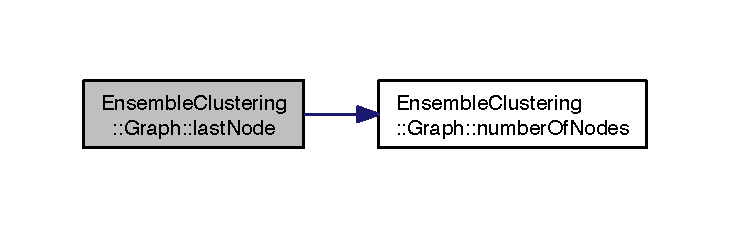
\includegraphics[width=350pt]{class_ensemble_clustering_1_1_graph_a3d6fe2d0c27605f4b55585198eb9b933_cgraph}
\end{center}
\end{figure}


\hypertarget{class_ensemble_clustering_1_1_graph_ab019840b239c3247eaf00e5ffcc6bb03}{\index{Ensemble\-Clustering\-::\-Graph@{Ensemble\-Clustering\-::\-Graph}!number\-Of\-Edges@{number\-Of\-Edges}}
\index{number\-Of\-Edges@{number\-Of\-Edges}!EnsembleClustering::Graph@{Ensemble\-Clustering\-::\-Graph}}
\subsubsection[{number\-Of\-Edges}]{\setlength{\rightskip}{0pt plus 5cm}int64\-\_\-t Ensemble\-Clustering\-::\-Graph\-::number\-Of\-Edges (
\begin{DoxyParamCaption}
{}
\end{DoxyParamCaption}
) const}}\label{class_ensemble_clustering_1_1_graph_ab019840b239c3247eaf00e5ffcc6bb03}


Return the number of edges in the graph. 



Definition at line 54 of file Graph.\-cpp.

\hypertarget{class_ensemble_clustering_1_1_graph_affe61a24e54266aba872272fb9501c61}{\index{Ensemble\-Clustering\-::\-Graph@{Ensemble\-Clustering\-::\-Graph}!number\-Of\-Nodes@{number\-Of\-Nodes}}
\index{number\-Of\-Nodes@{number\-Of\-Nodes}!EnsembleClustering::Graph@{Ensemble\-Clustering\-::\-Graph}}
\subsubsection[{number\-Of\-Nodes}]{\setlength{\rightskip}{0pt plus 5cm}int64\-\_\-t Ensemble\-Clustering\-::\-Graph\-::number\-Of\-Nodes (
\begin{DoxyParamCaption}
{}
\end{DoxyParamCaption}
) const}}\label{class_ensemble_clustering_1_1_graph_affe61a24e54266aba872272fb9501c61}


Return the number of (non-\/isolated) nodes in the graph. 

T\-O\-D\-O\-: Maybe this should be changed to support isolated nodes. 

Definition at line 59 of file Graph.\-cpp.

\hypertarget{class_ensemble_clustering_1_1_graph_a7be7f13f5a31b0513293e7bbac26ca6c}{\index{Ensemble\-Clustering\-::\-Graph@{Ensemble\-Clustering\-::\-Graph}!total\-Edge\-Weight@{total\-Edge\-Weight}}
\index{total\-Edge\-Weight@{total\-Edge\-Weight}!EnsembleClustering::Graph@{Ensemble\-Clustering\-::\-Graph}}
\subsubsection[{total\-Edge\-Weight}]{\setlength{\rightskip}{0pt plus 5cm}double Ensemble\-Clustering\-::\-Graph\-::total\-Edge\-Weight (
\begin{DoxyParamCaption}
{}
\end{DoxyParamCaption}
) const}}\label{class_ensemble_clustering_1_1_graph_a7be7f13f5a31b0513293e7bbac26ca6c}


Get the sum of the weight of all edges. 



Definition at line 76 of file Graph.\-cpp.



Here is the call graph for this function\-:\nopagebreak
\begin{figure}[H]
\begin{center}
\leavevmode
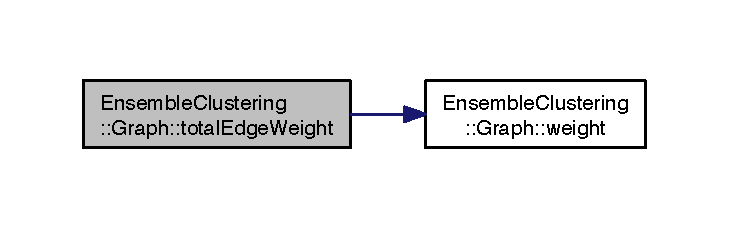
\includegraphics[width=350pt]{class_ensemble_clustering_1_1_graph_a7be7f13f5a31b0513293e7bbac26ca6c_cgraph}
\end{center}
\end{figure}


\hypertarget{class_ensemble_clustering_1_1_graph_a9bff231567f9ac604f1854d62f6682d1}{\index{Ensemble\-Clustering\-::\-Graph@{Ensemble\-Clustering\-::\-Graph}!weight@{weight}}
\index{weight@{weight}!EnsembleClustering::Graph@{Ensemble\-Clustering\-::\-Graph}}
\subsubsection[{weight}]{\setlength{\rightskip}{0pt plus 5cm}double Ensemble\-Clustering\-::\-Graph\-::weight (
\begin{DoxyParamCaption}
\item[{{\bf node}}]{v}
\end{DoxyParamCaption}
) const}}\label{class_ensemble_clustering_1_1_graph_a9bff231567f9ac604f1854d62f6682d1}


Return node weight. 



Definition at line 43 of file Graph.\-cpp.

\hypertarget{class_ensemble_clustering_1_1_graph_a656f5cb3119dd3f8f4182d38cce82fa0}{\index{Ensemble\-Clustering\-::\-Graph@{Ensemble\-Clustering\-::\-Graph}!weight@{weight}}
\index{weight@{weight}!EnsembleClustering::Graph@{Ensemble\-Clustering\-::\-Graph}}
\subsubsection[{weight}]{\setlength{\rightskip}{0pt plus 5cm}double Ensemble\-Clustering\-::\-Graph\-::weight (
\begin{DoxyParamCaption}
\item[{{\bf edge}}]{uv}
\end{DoxyParamCaption}
) const}}\label{class_ensemble_clustering_1_1_graph_a656f5cb3119dd3f8f4182d38cce82fa0}


Return edge weight. 



Definition at line 47 of file Graph.\-cpp.

\hypertarget{class_ensemble_clustering_1_1_graph_a4699131f4d3602ecda00eaf70a86cbea}{\index{Ensemble\-Clustering\-::\-Graph@{Ensemble\-Clustering\-::\-Graph}!weight@{weight}}
\index{weight@{weight}!EnsembleClustering::Graph@{Ensemble\-Clustering\-::\-Graph}}
\subsubsection[{weight}]{\setlength{\rightskip}{0pt plus 5cm}double Ensemble\-Clustering\-::\-Graph\-::weight (
\begin{DoxyParamCaption}
\item[{{\bf node}}]{u, }
\item[{{\bf node}}]{v}
\end{DoxyParamCaption}
) const\hspace{0.3cm}{\ttfamily [inline]}}}\label{class_ensemble_clustering_1_1_graph_a4699131f4d3602ecda00eaf70a86cbea}


Return edge weight. 

Equivalent to get\-Weight(edge uv) 

Definition at line 144 of file Graph.\-h.



\subsection{Member Data Documentation}
\hypertarget{class_ensemble_clustering_1_1_graph_a377621f37c1dc58f32ecec0fd229408e}{\index{Ensemble\-Clustering\-::\-Graph@{Ensemble\-Clustering\-::\-Graph}!default\-Edge\-Type@{default\-Edge\-Type}}
\index{default\-Edge\-Type@{default\-Edge\-Type}!EnsembleClustering::Graph@{Ensemble\-Clustering\-::\-Graph}}
\subsubsection[{default\-Edge\-Type}]{\setlength{\rightskip}{0pt plus 5cm}const int64\-\_\-t Ensemble\-Clustering\-::\-Graph\-::default\-Edge\-Type = 0\hspace{0.3cm}{\ttfamily [static]}}}\label{class_ensemble_clustering_1_1_graph_a377621f37c1dc58f32ecec0fd229408e}


Definition at line 92 of file Graph.\-h.

\hypertarget{class_ensemble_clustering_1_1_graph_a8186ee969064a4e12b779b1dc506ac60}{\index{Ensemble\-Clustering\-::\-Graph@{Ensemble\-Clustering\-::\-Graph}!default\-Edge\-Weight@{default\-Edge\-Weight}}
\index{default\-Edge\-Weight@{default\-Edge\-Weight}!EnsembleClustering::Graph@{Ensemble\-Clustering\-::\-Graph}}
\subsubsection[{default\-Edge\-Weight}]{\setlength{\rightskip}{0pt plus 5cm}constexpr double Ensemble\-Clustering\-::\-Graph\-::default\-Edge\-Weight = 1.\-0\hspace{0.3cm}{\ttfamily [static]}}}\label{class_ensemble_clustering_1_1_graph_a8186ee969064a4e12b779b1dc506ac60}


default parameters 



Definition at line 91 of file Graph.\-h.

\hypertarget{class_ensemble_clustering_1_1_graph_a9a6623d55f673a3b30e0c23284dd6da1}{\index{Ensemble\-Clustering\-::\-Graph@{Ensemble\-Clustering\-::\-Graph}!default\-Time\-Stamp@{default\-Time\-Stamp}}
\index{default\-Time\-Stamp@{default\-Time\-Stamp}!EnsembleClustering::Graph@{Ensemble\-Clustering\-::\-Graph}}
\subsubsection[{default\-Time\-Stamp}]{\setlength{\rightskip}{0pt plus 5cm}const int64\-\_\-t Ensemble\-Clustering\-::\-Graph\-::default\-Time\-Stamp = 0\hspace{0.3cm}{\ttfamily [static]}}}\label{class_ensemble_clustering_1_1_graph_a9a6623d55f673a3b30e0c23284dd6da1}


Definition at line 93 of file Graph.\-h.

\hypertarget{class_ensemble_clustering_1_1_graph_af83709e85afb91c70729405a725afb9a}{\index{Ensemble\-Clustering\-::\-Graph@{Ensemble\-Clustering\-::\-Graph}!stinger\-G@{stinger\-G}}
\index{stinger\-G@{stinger\-G}!EnsembleClustering::Graph@{Ensemble\-Clustering\-::\-Graph}}
\subsubsection[{stinger\-G}]{\setlength{\rightskip}{0pt plus 5cm}stinger$\ast$ Ensemble\-Clustering\-::\-Graph\-::stinger\-G\hspace{0.3cm}{\ttfamily [protected]}}}\label{class_ensemble_clustering_1_1_graph_af83709e85afb91c70729405a725afb9a}


Definition at line 81 of file Graph.\-h.



The documentation for this class was generated from the following files\-:\begin{DoxyCompactItemize}
\item 
src/graph/\hyperlink{_graph_8h}{Graph.\-h}\item 
src/graph/\hyperlink{_graph_8cpp}{Graph.\-cpp}\end{DoxyCompactItemize}

\hypertarget{class_ensemble_clustering_1_1_matching}{\section{Ensemble\-Clustering\-:\-:Matching Class Reference}
\label{class_ensemble_clustering_1_1_matching}\index{Ensemble\-Clustering\-::\-Matching@{Ensemble\-Clustering\-::\-Matching}}
}


{\ttfamily \#include $<$Matching.\-h$>$}



Inheritance diagram for Ensemble\-Clustering\-:\-:Matching\-:
\nopagebreak
\begin{figure}[H]
\begin{center}
\leavevmode
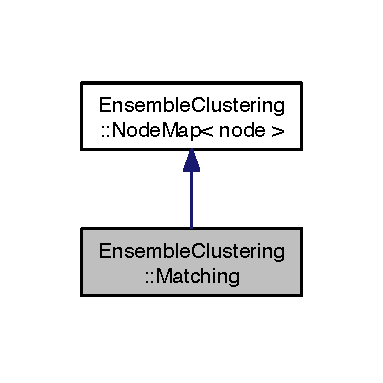
\includegraphics[width=212pt]{class_ensemble_clustering_1_1_matching__inherit__graph}
\end{center}
\end{figure}


Collaboration diagram for Ensemble\-Clustering\-:\-:Matching\-:
\nopagebreak
\begin{figure}[H]
\begin{center}
\leavevmode
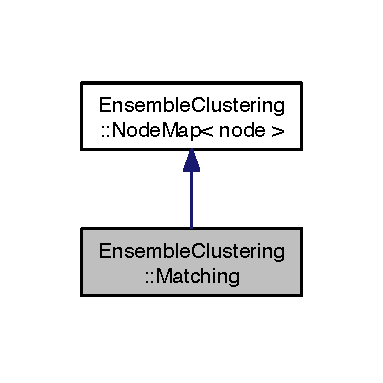
\includegraphics[width=212pt]{class_ensemble_clustering_1_1_matching__coll__graph}
\end{center}
\end{figure}
\subsection*{Public Member Functions}
\begin{DoxyCompactItemize}
\item 
\hyperlink{class_ensemble_clustering_1_1_matching_a5e1de8d09e758fae48909c25484b42b7}{Matching} (int64\-\_\-t \hyperlink{class_ensemble_clustering_1_1_index_map_a3151d302c54e6ad0175bd87aef62d4ca}{n})
\begin{DoxyCompactList}\small\item\em Construct new matching. \end{DoxyCompactList}\item 
virtual \hyperlink{class_ensemble_clustering_1_1_matching_abcc136cf0a7e0b0f2364f2d1b3eb1f2c}{$\sim$\-Matching} ()
\begin{DoxyCompactList}\small\item\em Destructor. \end{DoxyCompactList}\item 
void \hyperlink{class_ensemble_clustering_1_1_matching_a41f6ed1f3b1660fb682c32cf2ade11de}{match} (const \hyperlink{namespace_ensemble_clustering_ae829290aeccd1a420b17a37fd901f114}{node} \&u, const \hyperlink{namespace_ensemble_clustering_ae829290aeccd1a420b17a37fd901f114}{node} \&v)
\begin{DoxyCompactList}\small\item\em Set two nodes as eachothers matching partners. \end{DoxyCompactList}\item 
void \hyperlink{class_ensemble_clustering_1_1_matching_a214fd9e80cb5842f87e2ec909655b5e2}{unmatch} (const \hyperlink{namespace_ensemble_clustering_ae829290aeccd1a420b17a37fd901f114}{node} \&u, const \hyperlink{namespace_ensemble_clustering_ae829290aeccd1a420b17a37fd901f114}{node} \&v)
\begin{DoxyCompactList}\small\item\em Reset the two nodes to unmatched. \end{DoxyCompactList}\item 
bool \hyperlink{class_ensemble_clustering_1_1_matching_a6591583cd8dcd8ddc702cdbddcc42bd0}{is\-Matched} (const \hyperlink{namespace_ensemble_clustering_ae829290aeccd1a420b17a37fd901f114}{node} \&u) const 
\begin{DoxyCompactList}\small\item\em Check if node is matched. \end{DoxyCompactList}\item 
bool \hyperlink{class_ensemble_clustering_1_1_matching_ad2637dece8a3a56d9f62f3c9df4713db}{are\-Matched} (const \hyperlink{namespace_ensemble_clustering_ae829290aeccd1a420b17a37fd901f114}{node} \&u, const \hyperlink{namespace_ensemble_clustering_ae829290aeccd1a420b17a37fd901f114}{node} \&v) const 
\begin{DoxyCompactList}\small\item\em Check if the two nodes are matched. \end{DoxyCompactList}\item 
bool \hyperlink{class_ensemble_clustering_1_1_matching_a29b8fa3ba916f0b3d73b184c883c36b6}{is\-Proper} (\hyperlink{class_ensemble_clustering_1_1_graph}{Graph} \&G) const 
\begin{DoxyCompactList}\small\item\em Check whether this is a proper matching in the graph, i.\-e. \end{DoxyCompactList}\item 
\hyperlink{class_ensemble_clustering_1_1_matching}{Matching} \& \hyperlink{class_ensemble_clustering_1_1_matching_aa1d0732ec84c2012fd3e642595f23556}{operator=} (const \hyperlink{class_ensemble_clustering_1_1_matching}{Matching} \&from)
\begin{DoxyCompactList}\small\item\em copy semantics \end{DoxyCompactList}\item 
void \hyperlink{class_ensemble_clustering_1_1_matching_a6753fd67c53b6e0d94f2d6e0d6de640e}{clone} (const \hyperlink{class_ensemble_clustering_1_1_matching}{Matching} \&from)
\begin{DoxyCompactList}\small\item\em Properly copy this object. \end{DoxyCompactList}\item 
void \hyperlink{class_ensemble_clustering_1_1_matching_ae7e8c62662439dc7adae829506d2dd32}{dispose} ()
\begin{DoxyCompactList}\small\item\em Properly destruct this object. \end{DoxyCompactList}\item 
\hyperlink{namespace_ensemble_clustering_a2482e94ca22a0c6544a5a9173186fde8}{count} \hyperlink{class_ensemble_clustering_1_1_matching_a0e9020a85e9f6e8d0bf0ec236394b2e8}{matching\-Size} () const 
\item 
\hyperlink{namespace_ensemble_clustering_a1ba11e6d628873b803a26fe054f45e28}{index} \hyperlink{class_ensemble_clustering_1_1_matching_adc5f7971cb778e55e58b140e1371b89d}{mate} (\hyperlink{namespace_ensemble_clustering_ae829290aeccd1a420b17a37fd901f114}{node} v) const 
\end{DoxyCompactItemize}
\subsection*{Additional Inherited Members}


\subsection{Detailed Description}


Definition at line 17 of file Matching.\-h.



\subsection{Constructor \& Destructor Documentation}
\hypertarget{class_ensemble_clustering_1_1_matching_a5e1de8d09e758fae48909c25484b42b7}{\index{Ensemble\-Clustering\-::\-Matching@{Ensemble\-Clustering\-::\-Matching}!Matching@{Matching}}
\index{Matching@{Matching}!EnsembleClustering::Matching@{Ensemble\-Clustering\-::\-Matching}}
\subsubsection[{Matching}]{\setlength{\rightskip}{0pt plus 5cm}Ensemble\-Clustering\-::\-Matching\-::\-Matching (
\begin{DoxyParamCaption}
\item[{int64\-\_\-t}]{n}
\end{DoxyParamCaption}
)}}\label{class_ensemble_clustering_1_1_matching_a5e1de8d09e758fae48909c25484b42b7}


Construct new matching. 


\begin{DoxyParams}[1]{Parameters}
\mbox{\tt in}  & {\em n} & maximum number of nodes \\
\hline
\end{DoxyParams}


Definition at line 12 of file Matching.\-cpp.

\hypertarget{class_ensemble_clustering_1_1_matching_abcc136cf0a7e0b0f2364f2d1b3eb1f2c}{\index{Ensemble\-Clustering\-::\-Matching@{Ensemble\-Clustering\-::\-Matching}!$\sim$\-Matching@{$\sim$\-Matching}}
\index{$\sim$\-Matching@{$\sim$\-Matching}!EnsembleClustering::Matching@{Ensemble\-Clustering\-::\-Matching}}
\subsubsection[{$\sim$\-Matching}]{\setlength{\rightskip}{0pt plus 5cm}Ensemble\-Clustering\-::\-Matching\-::$\sim$\-Matching (
\begin{DoxyParamCaption}
{}
\end{DoxyParamCaption}
)\hspace{0.3cm}{\ttfamily [virtual]}}}\label{class_ensemble_clustering_1_1_matching_abcc136cf0a7e0b0f2364f2d1b3eb1f2c}


Destructor. 



Definition at line 20 of file Matching.\-cpp.



\subsection{Member Function Documentation}
\hypertarget{class_ensemble_clustering_1_1_matching_ad2637dece8a3a56d9f62f3c9df4713db}{\index{Ensemble\-Clustering\-::\-Matching@{Ensemble\-Clustering\-::\-Matching}!are\-Matched@{are\-Matched}}
\index{are\-Matched@{are\-Matched}!EnsembleClustering::Matching@{Ensemble\-Clustering\-::\-Matching}}
\subsubsection[{are\-Matched}]{\setlength{\rightskip}{0pt plus 5cm}bool Ensemble\-Clustering\-::\-Matching\-::are\-Matched (
\begin{DoxyParamCaption}
\item[{const {\bf node} \&}]{u, }
\item[{const {\bf node} \&}]{v}
\end{DoxyParamCaption}
) const}}\label{class_ensemble_clustering_1_1_matching_ad2637dece8a3a56d9f62f3c9df4713db}


Check if the two nodes are matched. 



Definition at line 70 of file Matching.\-cpp.

\hypertarget{class_ensemble_clustering_1_1_matching_a6753fd67c53b6e0d94f2d6e0d6de640e}{\index{Ensemble\-Clustering\-::\-Matching@{Ensemble\-Clustering\-::\-Matching}!clone@{clone}}
\index{clone@{clone}!EnsembleClustering::Matching@{Ensemble\-Clustering\-::\-Matching}}
\subsubsection[{clone}]{\setlength{\rightskip}{0pt plus 5cm}void Ensemble\-Clustering\-::\-Matching\-::clone (
\begin{DoxyParamCaption}
\item[{const {\bf Matching} \&}]{from}
\end{DoxyParamCaption}
)}}\label{class_ensemble_clustering_1_1_matching_a6753fd67c53b6e0d94f2d6e0d6de640e}


Properly copy this object. 

\hypertarget{class_ensemble_clustering_1_1_matching_ae7e8c62662439dc7adae829506d2dd32}{\index{Ensemble\-Clustering\-::\-Matching@{Ensemble\-Clustering\-::\-Matching}!dispose@{dispose}}
\index{dispose@{dispose}!EnsembleClustering::Matching@{Ensemble\-Clustering\-::\-Matching}}
\subsubsection[{dispose}]{\setlength{\rightskip}{0pt plus 5cm}void Ensemble\-Clustering\-::\-Matching\-::dispose (
\begin{DoxyParamCaption}
{}
\end{DoxyParamCaption}
)}}\label{class_ensemble_clustering_1_1_matching_ae7e8c62662439dc7adae829506d2dd32}


Properly destruct this object. 

\hypertarget{class_ensemble_clustering_1_1_matching_a6591583cd8dcd8ddc702cdbddcc42bd0}{\index{Ensemble\-Clustering\-::\-Matching@{Ensemble\-Clustering\-::\-Matching}!is\-Matched@{is\-Matched}}
\index{is\-Matched@{is\-Matched}!EnsembleClustering::Matching@{Ensemble\-Clustering\-::\-Matching}}
\subsubsection[{is\-Matched}]{\setlength{\rightskip}{0pt plus 5cm}bool Ensemble\-Clustering\-::\-Matching\-::is\-Matched (
\begin{DoxyParamCaption}
\item[{const {\bf node} \&}]{u}
\end{DoxyParamCaption}
) const}}\label{class_ensemble_clustering_1_1_matching_a6591583cd8dcd8ddc702cdbddcc42bd0}


Check if node is matched. 


\begin{DoxyParams}[1]{Parameters}
\mbox{\tt in}  & {\em u} & a node \\
\hline
\mbox{\tt out}  & {\em true} & if u is matched \\
\hline
\end{DoxyParams}


Definition at line 23 of file Matching.\-cpp.

\hypertarget{class_ensemble_clustering_1_1_matching_a29b8fa3ba916f0b3d73b184c883c36b6}{\index{Ensemble\-Clustering\-::\-Matching@{Ensemble\-Clustering\-::\-Matching}!is\-Proper@{is\-Proper}}
\index{is\-Proper@{is\-Proper}!EnsembleClustering::Matching@{Ensemble\-Clustering\-::\-Matching}}
\subsubsection[{is\-Proper}]{\setlength{\rightskip}{0pt plus 5cm}bool Ensemble\-Clustering\-::\-Matching\-::is\-Proper (
\begin{DoxyParamCaption}
\item[{{\bf Graph} \&}]{G}
\end{DoxyParamCaption}
) const}}\label{class_ensemble_clustering_1_1_matching_a29b8fa3ba916f0b3d73b184c883c36b6}


Check whether this is a proper matching in the graph, i.\-e. 

no two edges are adjacent.

\mbox{[}in\mbox{]} G a graph 
\begin{DoxyParams}[1]{Parameters}
\mbox{\tt out}  & {\em true} & if this is a proper matching \\
\hline
\end{DoxyParams}
The content of this data structure represents a matching iff (for all v in V\-: M\mbox{[}v\mbox{]} = v or M\mbox{[}M\mbox{[}v\mbox{]}\mbox{]} = v) and (for all (u,v) in M)\-: (u,v) in E

Definition at line 27 of file Matching.\-cpp.



Here is the call graph for this function\-:
\nopagebreak
\begin{figure}[H]
\begin{center}
\leavevmode
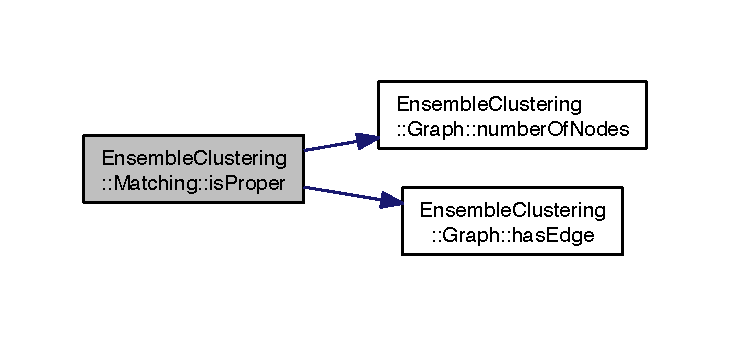
\includegraphics[width=350pt]{class_ensemble_clustering_1_1_matching_a29b8fa3ba916f0b3d73b184c883c36b6_cgraph}
\end{center}
\end{figure}


\hypertarget{class_ensemble_clustering_1_1_matching_a41f6ed1f3b1660fb682c32cf2ade11de}{\index{Ensemble\-Clustering\-::\-Matching@{Ensemble\-Clustering\-::\-Matching}!match@{match}}
\index{match@{match}!EnsembleClustering::Matching@{Ensemble\-Clustering\-::\-Matching}}
\subsubsection[{match}]{\setlength{\rightskip}{0pt plus 5cm}void Ensemble\-Clustering\-::\-Matching\-::match (
\begin{DoxyParamCaption}
\item[{const {\bf node} \&}]{u, }
\item[{const {\bf node} \&}]{v}
\end{DoxyParamCaption}
)}}\label{class_ensemble_clustering_1_1_matching_a41f6ed1f3b1660fb682c32cf2ade11de}


Set two nodes as eachothers matching partners. 



Definition at line 60 of file Matching.\-cpp.

\hypertarget{class_ensemble_clustering_1_1_matching_a0e9020a85e9f6e8d0bf0ec236394b2e8}{\index{Ensemble\-Clustering\-::\-Matching@{Ensemble\-Clustering\-::\-Matching}!matching\-Size@{matching\-Size}}
\index{matching\-Size@{matching\-Size}!EnsembleClustering::Matching@{Ensemble\-Clustering\-::\-Matching}}
\subsubsection[{matching\-Size}]{\setlength{\rightskip}{0pt plus 5cm}{\bf count} Ensemble\-Clustering\-::\-Matching\-::matching\-Size (
\begin{DoxyParamCaption}
{}
\end{DoxyParamCaption}
) const}}\label{class_ensemble_clustering_1_1_matching_a0e9020a85e9f6e8d0bf0ec236394b2e8}
\begin{DoxyReturn}{Returns}
Number of edges in matching. 
\end{DoxyReturn}


Definition at line 74 of file Matching.\-cpp.



Here is the call graph for this function\-:
\nopagebreak
\begin{figure}[H]
\begin{center}
\leavevmode
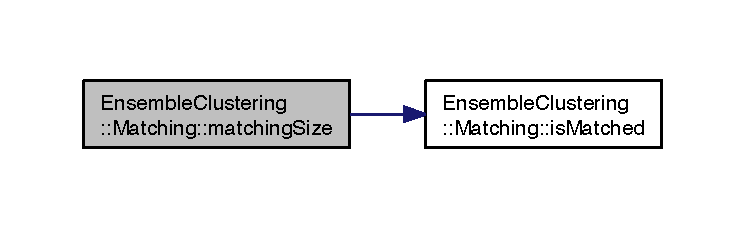
\includegraphics[width=350pt]{class_ensemble_clustering_1_1_matching_a0e9020a85e9f6e8d0bf0ec236394b2e8_cgraph}
\end{center}
\end{figure}


\hypertarget{class_ensemble_clustering_1_1_matching_adc5f7971cb778e55e58b140e1371b89d}{\index{Ensemble\-Clustering\-::\-Matching@{Ensemble\-Clustering\-::\-Matching}!mate@{mate}}
\index{mate@{mate}!EnsembleClustering::Matching@{Ensemble\-Clustering\-::\-Matching}}
\subsubsection[{mate}]{\setlength{\rightskip}{0pt plus 5cm}{\bf index} Ensemble\-Clustering\-::\-Matching\-::mate (
\begin{DoxyParamCaption}
\item[{{\bf node}}]{v}
\end{DoxyParamCaption}
) const}}\label{class_ensemble_clustering_1_1_matching_adc5f7971cb778e55e58b140e1371b89d}
\begin{DoxyReturn}{Returns}
Mate of {\itshape v} if it exists, otherwise none. 
\end{DoxyReturn}


Definition at line 84 of file Matching.\-cpp.



Here is the call graph for this function\-:
\nopagebreak
\begin{figure}[H]
\begin{center}
\leavevmode
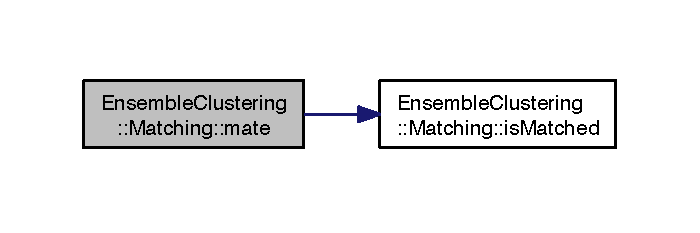
\includegraphics[width=336pt]{class_ensemble_clustering_1_1_matching_adc5f7971cb778e55e58b140e1371b89d_cgraph}
\end{center}
\end{figure}


\hypertarget{class_ensemble_clustering_1_1_matching_aa1d0732ec84c2012fd3e642595f23556}{\index{Ensemble\-Clustering\-::\-Matching@{Ensemble\-Clustering\-::\-Matching}!operator=@{operator=}}
\index{operator=@{operator=}!EnsembleClustering::Matching@{Ensemble\-Clustering\-::\-Matching}}
\subsubsection[{operator=}]{\setlength{\rightskip}{0pt plus 5cm}{\bf Matching}\& Ensemble\-Clustering\-::\-Matching\-::operator= (
\begin{DoxyParamCaption}
\item[{const {\bf Matching} \&}]{from}
\end{DoxyParamCaption}
)}}\label{class_ensemble_clustering_1_1_matching_aa1d0732ec84c2012fd3e642595f23556}


copy semantics 

Assignment operator. \hypertarget{class_ensemble_clustering_1_1_matching_a214fd9e80cb5842f87e2ec909655b5e2}{\index{Ensemble\-Clustering\-::\-Matching@{Ensemble\-Clustering\-::\-Matching}!unmatch@{unmatch}}
\index{unmatch@{unmatch}!EnsembleClustering::Matching@{Ensemble\-Clustering\-::\-Matching}}
\subsubsection[{unmatch}]{\setlength{\rightskip}{0pt plus 5cm}void Ensemble\-Clustering\-::\-Matching\-::unmatch (
\begin{DoxyParamCaption}
\item[{const {\bf node} \&}]{u, }
\item[{const {\bf node} \&}]{v}
\end{DoxyParamCaption}
)}}\label{class_ensemble_clustering_1_1_matching_a214fd9e80cb5842f87e2ec909655b5e2}


Reset the two nodes to unmatched. 



Definition at line 65 of file Matching.\-cpp.



The documentation for this class was generated from the following files\-:\begin{DoxyCompactItemize}
\item 
src/matching/\hyperlink{_matching_8h}{Matching.\-h}\item 
src/matching/\hyperlink{_matching_8cpp}{Matching.\-cpp}\end{DoxyCompactItemize}

\hypertarget{class_ensemble_clustering_1_1_m_e_t_i_s_graph_parser}{\section{Ensemble\-Clustering\-:\-:M\-E\-T\-I\-S\-Graph\-Parser Class Reference}
\label{class_ensemble_clustering_1_1_m_e_t_i_s_graph_parser}\index{Ensemble\-Clustering\-::\-M\-E\-T\-I\-S\-Graph\-Parser@{Ensemble\-Clustering\-::\-M\-E\-T\-I\-S\-Graph\-Parser}}
}


A parser for the M\-E\-T\-I\-S graph file format.  




{\ttfamily \#include $<$M\-E\-T\-I\-S\-Graph\-Parser.\-h$>$}

\subsection*{Public Member Functions}
\begin{DoxyCompactItemize}
\item 
\hyperlink{class_ensemble_clustering_1_1_m_e_t_i_s_graph_parser_a368585c6c1b9cfd6e95bd3ddd6547792}{M\-E\-T\-I\-S\-Graph\-Parser} ()
\item 
virtual \hyperlink{class_ensemble_clustering_1_1_m_e_t_i_s_graph_parser_a6d946610b24a1ed6cfe996379d3e5284}{$\sim$\-M\-E\-T\-I\-S\-Graph\-Parser} ()
\item 
virtual \hyperlink{class_ensemble_clustering_1_1_graph}{Graph} \hyperlink{class_ensemble_clustering_1_1_m_e_t_i_s_graph_parser_a28c963c44b2a559f1f26a68ce55b8650}{parse} (std\-::string path)
\begin{DoxyCompactList}\small\item\em Parses and returns a graph from a M\-E\-T\-I\-S graph file. \end{DoxyCompactList}\end{DoxyCompactItemize}
\subsection*{Protected Member Functions}
\begin{DoxyCompactItemize}
\item 
virtual void \hyperlink{class_ensemble_clustering_1_1_m_e_t_i_s_graph_parser_ad78da77d9f2eba97f3f3b755c18cf4ba}{init\-Graph} (int n, int m)
\begin{DoxyCompactList}\small\item\em Initializes the graph data structure before parsing. \end{DoxyCompactList}\item 
virtual void \hyperlink{class_ensemble_clustering_1_1_m_e_t_i_s_graph_parser_a7108ff92f806af29c49461f7e117ebbe}{connect\-Node} (\hyperlink{namespace_ensemble_clustering_a3228848abf8dfd6602f3b08dd459ea20}{id} v, std\-::vector$<$ \hyperlink{namespace_ensemble_clustering_a3228848abf8dfd6602f3b08dd459ea20}{id} $>$ indices)
\begin{DoxyCompactList}\small\item\em Connects node with to all its neighbors. \end{DoxyCompactList}\end{DoxyCompactItemize}


\subsection{Detailed Description}
A parser for the M\-E\-T\-I\-S graph file format. 

{\bfseries M\-E\-T\-I\-S graph file format}


\begin{DoxyItemize}
\item A\-S\-C\-I\-I
\item a graph of N nodes is stored in a file of N+1 lines;
\item the first line lists the number of nodes and the number of edges;
\item If the first line contains more than two values, the extra values indicate the weights;
\item each subsequent line lists the \char`\"{}neighbors\char`\"{} of a node;
\item comment lines begin with a \char`\"{}\%\char`\"{} sign; 
\end{DoxyItemize}

Definition at line 37 of file M\-E\-T\-I\-S\-Graph\-Parser.\-h.



\subsection{Constructor \& Destructor Documentation}
\hypertarget{class_ensemble_clustering_1_1_m_e_t_i_s_graph_parser_a368585c6c1b9cfd6e95bd3ddd6547792}{\index{Ensemble\-Clustering\-::\-M\-E\-T\-I\-S\-Graph\-Parser@{Ensemble\-Clustering\-::\-M\-E\-T\-I\-S\-Graph\-Parser}!M\-E\-T\-I\-S\-Graph\-Parser@{M\-E\-T\-I\-S\-Graph\-Parser}}
\index{M\-E\-T\-I\-S\-Graph\-Parser@{M\-E\-T\-I\-S\-Graph\-Parser}!EnsembleClustering::METISGraphParser@{Ensemble\-Clustering\-::\-M\-E\-T\-I\-S\-Graph\-Parser}}
\subsubsection[{M\-E\-T\-I\-S\-Graph\-Parser}]{\setlength{\rightskip}{0pt plus 5cm}Ensemble\-Clustering\-::\-M\-E\-T\-I\-S\-Graph\-Parser\-::\-M\-E\-T\-I\-S\-Graph\-Parser (
\begin{DoxyParamCaption}
{}
\end{DoxyParamCaption}
)}}\label{class_ensemble_clustering_1_1_m_e_t_i_s_graph_parser_a368585c6c1b9cfd6e95bd3ddd6547792}


Definition at line 19 of file M\-E\-T\-I\-S\-Graph\-Parser.\-cpp.

\hypertarget{class_ensemble_clustering_1_1_m_e_t_i_s_graph_parser_a6d946610b24a1ed6cfe996379d3e5284}{\index{Ensemble\-Clustering\-::\-M\-E\-T\-I\-S\-Graph\-Parser@{Ensemble\-Clustering\-::\-M\-E\-T\-I\-S\-Graph\-Parser}!$\sim$\-M\-E\-T\-I\-S\-Graph\-Parser@{$\sim$\-M\-E\-T\-I\-S\-Graph\-Parser}}
\index{$\sim$\-M\-E\-T\-I\-S\-Graph\-Parser@{$\sim$\-M\-E\-T\-I\-S\-Graph\-Parser}!EnsembleClustering::METISGraphParser@{Ensemble\-Clustering\-::\-M\-E\-T\-I\-S\-Graph\-Parser}}
\subsubsection[{$\sim$\-M\-E\-T\-I\-S\-Graph\-Parser}]{\setlength{\rightskip}{0pt plus 5cm}Ensemble\-Clustering\-::\-M\-E\-T\-I\-S\-Graph\-Parser\-::$\sim$\-M\-E\-T\-I\-S\-Graph\-Parser (
\begin{DoxyParamCaption}
{}
\end{DoxyParamCaption}
)\hspace{0.3cm}{\ttfamily [virtual]}}}\label{class_ensemble_clustering_1_1_m_e_t_i_s_graph_parser_a6d946610b24a1ed6cfe996379d3e5284}


Definition at line 24 of file M\-E\-T\-I\-S\-Graph\-Parser.\-cpp.



\subsection{Member Function Documentation}
\hypertarget{class_ensemble_clustering_1_1_m_e_t_i_s_graph_parser_a7108ff92f806af29c49461f7e117ebbe}{\index{Ensemble\-Clustering\-::\-M\-E\-T\-I\-S\-Graph\-Parser@{Ensemble\-Clustering\-::\-M\-E\-T\-I\-S\-Graph\-Parser}!connect\-Node@{connect\-Node}}
\index{connect\-Node@{connect\-Node}!EnsembleClustering::METISGraphParser@{Ensemble\-Clustering\-::\-M\-E\-T\-I\-S\-Graph\-Parser}}
\subsubsection[{connect\-Node}]{\setlength{\rightskip}{0pt plus 5cm}void Ensemble\-Clustering\-::\-M\-E\-T\-I\-S\-Graph\-Parser\-::connect\-Node (
\begin{DoxyParamCaption}
\item[{{\bf id}}]{v, }
\item[{std\-::vector$<$ {\bf id} $>$}]{indices}
\end{DoxyParamCaption}
)\hspace{0.3cm}{\ttfamily [protected]}, {\ttfamily [virtual]}}}\label{class_ensemble_clustering_1_1_m_e_t_i_s_graph_parser_a7108ff92f806af29c49461f7e117ebbe}


Connects node with to all its neighbors. 


\begin{DoxyParams}[1]{Parameters}
\mbox{\tt in}  & {\em v} & node id \\
\hline
\mbox{\tt in}  & {\em indices} & neighbor node ids \\
\hline
\end{DoxyParams}


Definition at line 111 of file M\-E\-T\-I\-S\-Graph\-Parser.\-cpp.

\hypertarget{class_ensemble_clustering_1_1_m_e_t_i_s_graph_parser_ad78da77d9f2eba97f3f3b755c18cf4ba}{\index{Ensemble\-Clustering\-::\-M\-E\-T\-I\-S\-Graph\-Parser@{Ensemble\-Clustering\-::\-M\-E\-T\-I\-S\-Graph\-Parser}!init\-Graph@{init\-Graph}}
\index{init\-Graph@{init\-Graph}!EnsembleClustering::METISGraphParser@{Ensemble\-Clustering\-::\-M\-E\-T\-I\-S\-Graph\-Parser}}
\subsubsection[{init\-Graph}]{\setlength{\rightskip}{0pt plus 5cm}void Ensemble\-Clustering\-::\-M\-E\-T\-I\-S\-Graph\-Parser\-::init\-Graph (
\begin{DoxyParamCaption}
\item[{int}]{n, }
\item[{int}]{m}
\end{DoxyParamCaption}
)\hspace{0.3cm}{\ttfamily [protected]}, {\ttfamily [virtual]}}}\label{class_ensemble_clustering_1_1_m_e_t_i_s_graph_parser_ad78da77d9f2eba97f3f3b755c18cf4ba}


Initializes the graph data structure before parsing. 



Definition at line 103 of file M\-E\-T\-I\-S\-Graph\-Parser.\-cpp.

\hypertarget{class_ensemble_clustering_1_1_m_e_t_i_s_graph_parser_a28c963c44b2a559f1f26a68ce55b8650}{\index{Ensemble\-Clustering\-::\-M\-E\-T\-I\-S\-Graph\-Parser@{Ensemble\-Clustering\-::\-M\-E\-T\-I\-S\-Graph\-Parser}!parse@{parse}}
\index{parse@{parse}!EnsembleClustering::METISGraphParser@{Ensemble\-Clustering\-::\-M\-E\-T\-I\-S\-Graph\-Parser}}
\subsubsection[{parse}]{\setlength{\rightskip}{0pt plus 5cm}{\bf Graph} Ensemble\-Clustering\-::\-M\-E\-T\-I\-S\-Graph\-Parser\-::parse (
\begin{DoxyParamCaption}
\item[{std\-::string}]{path}
\end{DoxyParamCaption}
)\hspace{0.3cm}{\ttfamily [virtual]}}}\label{class_ensemble_clustering_1_1_m_e_t_i_s_graph_parser_a28c963c44b2a559f1f26a68ce55b8650}


Parses and returns a graph from a M\-E\-T\-I\-S graph file. 


\begin{DoxyParams}[1]{Parameters}
\mbox{\tt in}  & {\em path} & path of the M\-E\-T\-I\-S graph input file\\
\hline
\mbox{\tt out}  & {\em graph} & the graph contained in the input file \\
\hline
\end{DoxyParams}


Definition at line 54 of file M\-E\-T\-I\-S\-Graph\-Parser.\-cpp.



The documentation for this class was generated from the following files\-:\begin{DoxyCompactItemize}
\item 
src/\hyperlink{_m_e_t_i_s_graph_parser_8h}{M\-E\-T\-I\-S\-Graph\-Parser.\-h}\item 
src/\hyperlink{_m_e_t_i_s_graph_parser_8cpp}{M\-E\-T\-I\-S\-Graph\-Parser.\-cpp}\end{DoxyCompactItemize}

\hypertarget{class_ensemble_clustering_1_1_modularity}{\section{Ensemble\-Clustering\-:\-:Modularity Class Reference}
\label{class_ensemble_clustering_1_1_modularity}\index{Ensemble\-Clustering\-::\-Modularity@{Ensemble\-Clustering\-::\-Modularity}}
}


{\ttfamily \#include $<$Modularity.\-h$>$}



Inheritance diagram for Ensemble\-Clustering\-:\-:Modularity\-:\nopagebreak
\begin{figure}[H]
\begin{center}
\leavevmode
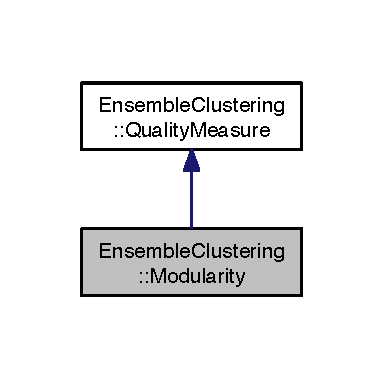
\includegraphics[width=184pt]{class_ensemble_clustering_1_1_modularity__inherit__graph}
\end{center}
\end{figure}


Collaboration diagram for Ensemble\-Clustering\-:\-:Modularity\-:\nopagebreak
\begin{figure}[H]
\begin{center}
\leavevmode
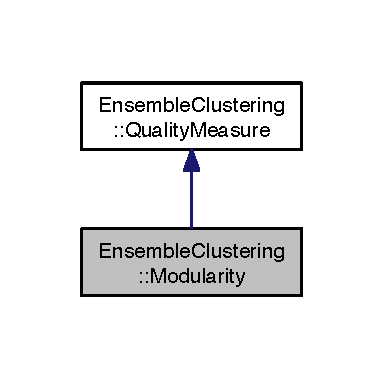
\includegraphics[width=315pt]{class_ensemble_clustering_1_1_modularity__coll__graph}
\end{center}
\end{figure}
\subsection*{Public Member Functions}
\begin{DoxyCompactItemize}
\item 
\hyperlink{class_ensemble_clustering_1_1_modularity_ac2cac4e5a1aa00af4fce69123c57f94b}{Modularity} (\hyperlink{class_ensemble_clustering_1_1_graph}{Graph} \&\hyperlink{class_ensemble_clustering_1_1_quality_measure_a8639730658036901338b34bc59bf4cec}{G})
\item 
virtual \hyperlink{class_ensemble_clustering_1_1_modularity_a57b3f96bdd38a7920317e7587518715d}{$\sim$\-Modularity} ()
\item 
virtual double \hyperlink{class_ensemble_clustering_1_1_modularity_a516c1fa49609c233d01a76d0f0d4c255}{get\-Quality} (\hyperlink{class_ensemble_clustering_1_1_clustering}{Clustering} \&zeta)
\begin{DoxyCompactList}\small\item\em Returns the \hyperlink{class_ensemble_clustering_1_1_modularity}{Modularity} of the given clustering with respect to the graph instance. \end{DoxyCompactList}\end{DoxyCompactItemize}
\subsection*{Protected Member Functions}
\begin{DoxyCompactItemize}
\item 
virtual void \hyperlink{class_ensemble_clustering_1_1_modularity_a5c449dd6b3b3485dcc497edd8dc3c156}{precompute} ()
\begin{DoxyCompactList}\small\item\em Precompute some values depending on the graph instance to be used in get\-Quality. \end{DoxyCompactList}\end{DoxyCompactItemize}
\subsection*{Protected Attributes}
\begin{DoxyCompactItemize}
\item 
\hyperlink{class_ensemble_clustering_1_1_node_map}{Node\-Map}$<$ double $>$ $\ast$ \hyperlink{class_ensemble_clustering_1_1_modularity_abc6c72d596cd3f00cce8c8c87e602df1}{incident\-Weight}
\begin{DoxyCompactList}\small\item\em node -\/$>$ sum of the weight of incident edges \end{DoxyCompactList}\end{DoxyCompactItemize}


\subsection{Detailed Description}


Definition at line 22 of file Modularity.\-h.



\subsection{Constructor \& Destructor Documentation}
\hypertarget{class_ensemble_clustering_1_1_modularity_ac2cac4e5a1aa00af4fce69123c57f94b}{\index{Ensemble\-Clustering\-::\-Modularity@{Ensemble\-Clustering\-::\-Modularity}!Modularity@{Modularity}}
\index{Modularity@{Modularity}!EnsembleClustering::Modularity@{Ensemble\-Clustering\-::\-Modularity}}
\subsubsection[{Modularity}]{\setlength{\rightskip}{0pt plus 5cm}Ensemble\-Clustering\-::\-Modularity\-::\-Modularity (
\begin{DoxyParamCaption}
\item[{{\bf Graph} \&}]{G}
\end{DoxyParamCaption}
)}}\label{class_ensemble_clustering_1_1_modularity_ac2cac4e5a1aa00af4fce69123c57f94b}


Definition at line 14 of file Modularity.\-cpp.



Here is the call graph for this function\-:\nopagebreak
\begin{figure}[H]
\begin{center}
\leavevmode
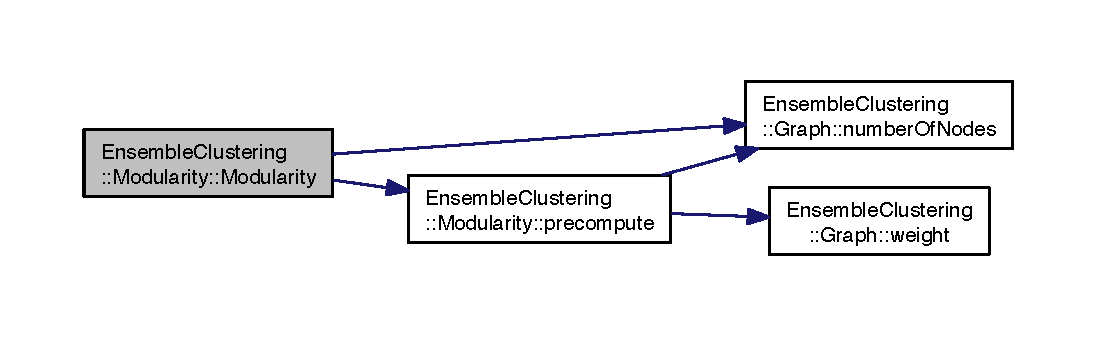
\includegraphics[width=350pt]{class_ensemble_clustering_1_1_modularity_ac2cac4e5a1aa00af4fce69123c57f94b_cgraph}
\end{center}
\end{figure}


\hypertarget{class_ensemble_clustering_1_1_modularity_a57b3f96bdd38a7920317e7587518715d}{\index{Ensemble\-Clustering\-::\-Modularity@{Ensemble\-Clustering\-::\-Modularity}!$\sim$\-Modularity@{$\sim$\-Modularity}}
\index{$\sim$\-Modularity@{$\sim$\-Modularity}!EnsembleClustering::Modularity@{Ensemble\-Clustering\-::\-Modularity}}
\subsubsection[{$\sim$\-Modularity}]{\setlength{\rightskip}{0pt plus 5cm}Ensemble\-Clustering\-::\-Modularity\-::$\sim$\-Modularity (
\begin{DoxyParamCaption}
{}
\end{DoxyParamCaption}
)\hspace{0.3cm}{\ttfamily [virtual]}}}\label{class_ensemble_clustering_1_1_modularity_a57b3f96bdd38a7920317e7587518715d}


Definition at line 19 of file Modularity.\-cpp.



\subsection{Member Function Documentation}
\hypertarget{class_ensemble_clustering_1_1_modularity_a516c1fa49609c233d01a76d0f0d4c255}{\index{Ensemble\-Clustering\-::\-Modularity@{Ensemble\-Clustering\-::\-Modularity}!get\-Quality@{get\-Quality}}
\index{get\-Quality@{get\-Quality}!EnsembleClustering::Modularity@{Ensemble\-Clustering\-::\-Modularity}}
\subsubsection[{get\-Quality}]{\setlength{\rightskip}{0pt plus 5cm}double Ensemble\-Clustering\-::\-Modularity\-::get\-Quality (
\begin{DoxyParamCaption}
\item[{{\bf Clustering} \&}]{zeta}
\end{DoxyParamCaption}
)\hspace{0.3cm}{\ttfamily [virtual]}}}\label{class_ensemble_clustering_1_1_modularity_a516c1fa49609c233d01a76d0f0d4c255}


Returns the \hyperlink{class_ensemble_clustering_1_1_modularity}{Modularity} of the given clustering with respect to the graph instance. 

\hyperlink{class_ensemble_clustering_1_1_modularity}{Modularity} is defined as\-: \begin{DoxyVerb}$$mod(\zeta) := \frac{\sum_{C \in \zeta} \sum_{ e \in E(C) } \omega(e)}{\sum_{e \in E} \omega(e)}
- \frac{ \sum_{C \in \zeta}( \sum_{v \in C} \omega(v) )^2 }{4( \sum_{e \in E} \omega(e) )^2 }$$\end{DoxyVerb}
 $<$ term \$\{\{C  \} \{ e  E(\-C) \} (e)\}\{\{e  E\} (e)\}\$

$<$ term \$\{ \{C  \}( \{v  C\} (v) )$^\wedge$2 \}\{4( \{e  E\} (e) )$^\wedge$2 \}\$

$<$ cluster -\/$>$ weight of its internal edges

$<$ term \$\{C  \} \{ e  E(\-C) \} (e)\$

$<$ cluster -\/$>$ sum of the weights of incident edges for all nodes

$<$ term \$\{C  \}( \{v  C\} (v) )$^\wedge$2 \$ 

Implements \hyperlink{class_ensemble_clustering_1_1_quality_measure_ac451b559397c922c27be3a64b3463bd9}{Ensemble\-Clustering\-::\-Quality\-Measure}.



Definition at line 36 of file Modularity.\-cpp.



Here is the call graph for this function\-:\nopagebreak
\begin{figure}[H]
\begin{center}
\leavevmode
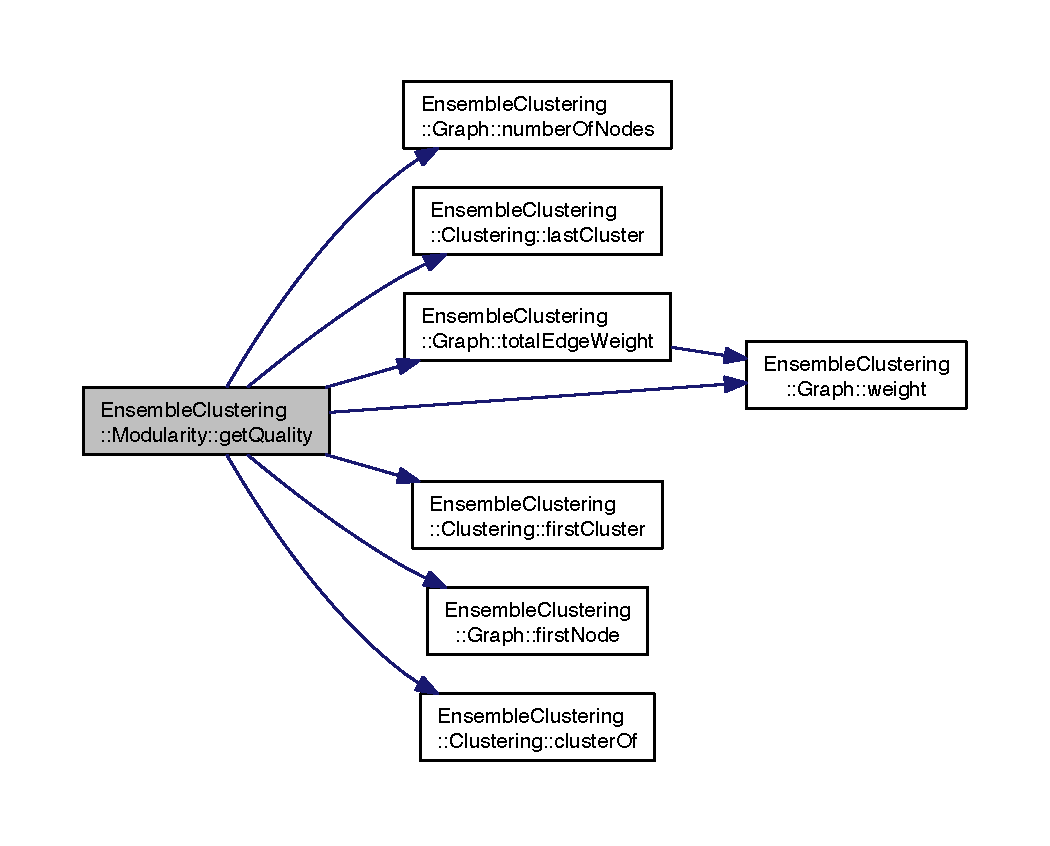
\includegraphics[width=350pt]{class_ensemble_clustering_1_1_modularity_a516c1fa49609c233d01a76d0f0d4c255_cgraph}
\end{center}
\end{figure}


\hypertarget{class_ensemble_clustering_1_1_modularity_a5c449dd6b3b3485dcc497edd8dc3c156}{\index{Ensemble\-Clustering\-::\-Modularity@{Ensemble\-Clustering\-::\-Modularity}!precompute@{precompute}}
\index{precompute@{precompute}!EnsembleClustering::Modularity@{Ensemble\-Clustering\-::\-Modularity}}
\subsubsection[{precompute}]{\setlength{\rightskip}{0pt plus 5cm}void Ensemble\-Clustering\-::\-Modularity\-::precompute (
\begin{DoxyParamCaption}
{}
\end{DoxyParamCaption}
)\hspace{0.3cm}{\ttfamily [protected]}, {\ttfamily [virtual]}}}\label{class_ensemble_clustering_1_1_modularity_a5c449dd6b3b3485dcc497edd8dc3c156}


Precompute some values depending on the graph instance to be used in get\-Quality. 



Definition at line 23 of file Modularity.\-cpp.



Here is the call graph for this function\-:\nopagebreak
\begin{figure}[H]
\begin{center}
\leavevmode
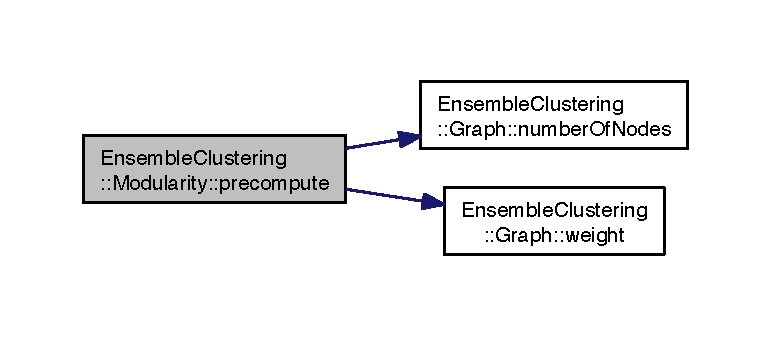
\includegraphics[width=350pt]{class_ensemble_clustering_1_1_modularity_a5c449dd6b3b3485dcc497edd8dc3c156_cgraph}
\end{center}
\end{figure}




\subsection{Member Data Documentation}
\hypertarget{class_ensemble_clustering_1_1_modularity_abc6c72d596cd3f00cce8c8c87e602df1}{\index{Ensemble\-Clustering\-::\-Modularity@{Ensemble\-Clustering\-::\-Modularity}!incident\-Weight@{incident\-Weight}}
\index{incident\-Weight@{incident\-Weight}!EnsembleClustering::Modularity@{Ensemble\-Clustering\-::\-Modularity}}
\subsubsection[{incident\-Weight}]{\setlength{\rightskip}{0pt plus 5cm}{\bf Node\-Map}$<$double$>$$\ast$ Ensemble\-Clustering\-::\-Modularity\-::incident\-Weight\hspace{0.3cm}{\ttfamily [protected]}}}\label{class_ensemble_clustering_1_1_modularity_abc6c72d596cd3f00cce8c8c87e602df1}


node -\/$>$ sum of the weight of incident edges 



Definition at line 26 of file Modularity.\-h.



The documentation for this class was generated from the following files\-:\begin{DoxyCompactItemize}
\item 
src/clustering/\hyperlink{_modularity_8h}{Modularity.\-h}\item 
src/clustering/\hyperlink{_modularity_8cpp}{Modularity.\-cpp}\end{DoxyCompactItemize}

\hypertarget{class_ensemble_clustering_1_1_node_tuple}{\section{Ensemble\-Clustering\-:\-:Node\-Tuple Class Reference}
\label{class_ensemble_clustering_1_1_node_tuple}\index{Ensemble\-Clustering\-::\-Node\-Tuple@{Ensemble\-Clustering\-::\-Node\-Tuple}}
}


{\ttfamily \#include $<$Edge\-Triple\-Graph\-Data.\-h$>$}

\subsection*{Public Member Functions}
\begin{DoxyCompactItemize}
\item 
\hyperlink{class_ensemble_clustering_1_1_node_tuple_a13bad67e06f1a1ec63c595b677afe597}{Node\-Tuple} ()
\item 
\hyperlink{class_ensemble_clustering_1_1_node_tuple_a76e905b5c712fc25f8b7b27f72f7c897}{Node\-Tuple} (double \hyperlink{class_ensemble_clustering_1_1_node_tuple_ad22f4e0e736249fe884f9adb87491d66}{w})
\end{DoxyCompactItemize}
\subsection*{Public Attributes}
\begin{DoxyCompactItemize}
\item 
double \hyperlink{class_ensemble_clustering_1_1_node_tuple_ad22f4e0e736249fe884f9adb87491d66}{w}
\begin{DoxyCompactList}\small\item\em self-\/loop weight \end{DoxyCompactList}\end{DoxyCompactItemize}


\subsection{Detailed Description}


Definition at line 36 of file Edge\-Triple\-Graph\-Data.\-h.



\subsection{Constructor \& Destructor Documentation}
\hypertarget{class_ensemble_clustering_1_1_node_tuple_a13bad67e06f1a1ec63c595b677afe597}{\index{Ensemble\-Clustering\-::\-Node\-Tuple@{Ensemble\-Clustering\-::\-Node\-Tuple}!Node\-Tuple@{Node\-Tuple}}
\index{Node\-Tuple@{Node\-Tuple}!EnsembleClustering::NodeTuple@{Ensemble\-Clustering\-::\-Node\-Tuple}}
\subsubsection[{Node\-Tuple}]{\setlength{\rightskip}{0pt plus 5cm}Ensemble\-Clustering\-::\-Node\-Tuple\-::\-Node\-Tuple (
\begin{DoxyParamCaption}
{}
\end{DoxyParamCaption}
)}}\label{class_ensemble_clustering_1_1_node_tuple_a13bad67e06f1a1ec63c595b677afe597}


Definition at line 25 of file Edge\-Triple\-Graph\-Data.\-cpp.

\hypertarget{class_ensemble_clustering_1_1_node_tuple_a76e905b5c712fc25f8b7b27f72f7c897}{\index{Ensemble\-Clustering\-::\-Node\-Tuple@{Ensemble\-Clustering\-::\-Node\-Tuple}!Node\-Tuple@{Node\-Tuple}}
\index{Node\-Tuple@{Node\-Tuple}!EnsembleClustering::NodeTuple@{Ensemble\-Clustering\-::\-Node\-Tuple}}
\subsubsection[{Node\-Tuple}]{\setlength{\rightskip}{0pt plus 5cm}Ensemble\-Clustering\-::\-Node\-Tuple\-::\-Node\-Tuple (
\begin{DoxyParamCaption}
\item[{double}]{w}
\end{DoxyParamCaption}
)}}\label{class_ensemble_clustering_1_1_node_tuple_a76e905b5c712fc25f8b7b27f72f7c897}


Definition at line 29 of file Edge\-Triple\-Graph\-Data.\-cpp.



\subsection{Member Data Documentation}
\hypertarget{class_ensemble_clustering_1_1_node_tuple_ad22f4e0e736249fe884f9adb87491d66}{\index{Ensemble\-Clustering\-::\-Node\-Tuple@{Ensemble\-Clustering\-::\-Node\-Tuple}!w@{w}}
\index{w@{w}!EnsembleClustering::NodeTuple@{Ensemble\-Clustering\-::\-Node\-Tuple}}
\subsubsection[{w}]{\setlength{\rightskip}{0pt plus 5cm}double Ensemble\-Clustering\-::\-Node\-Tuple\-::w}}\label{class_ensemble_clustering_1_1_node_tuple_ad22f4e0e736249fe884f9adb87491d66}


self-\/loop weight 



Definition at line 44 of file Edge\-Triple\-Graph\-Data.\-h.



The documentation for this class was generated from the following files\-:\begin{DoxyCompactItemize}
\item 
src/\hyperlink{_edge_triple_graph_data_8h}{Edge\-Triple\-Graph\-Data.\-h}\item 
src/\hyperlink{_edge_triple_graph_data_8cpp}{Edge\-Triple\-Graph\-Data.\-cpp}\end{DoxyCompactItemize}

\chapter{File Documentation}
\hypertarget{_edge_scoring_8cpp}{\section{src/scoring/\-Edge\-Scoring.cpp File Reference}
\label{_edge_scoring_8cpp}\index{src/scoring/\-Edge\-Scoring.\-cpp@{src/scoring/\-Edge\-Scoring.\-cpp}}
}
{\ttfamily \#include \char`\"{}Edge\-Scoring.\-h\char`\"{}}\\*
Include dependency graph for Edge\-Scoring.\-cpp\-:\nopagebreak
\begin{figure}[H]
\begin{center}
\leavevmode
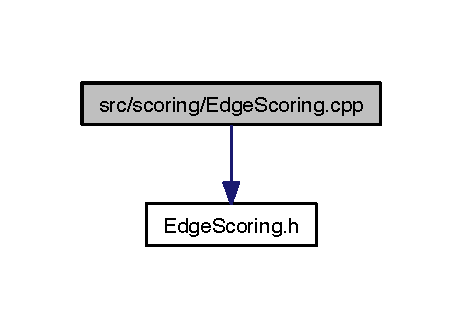
\includegraphics[width=350pt]{_edge_scoring_8cpp__incl}
\end{center}
\end{figure}
\subsection*{Namespaces}
\begin{DoxyCompactItemize}
\item 
\hyperlink{namespace_networ_kit}{Networ\-Kit}
\end{DoxyCompactItemize}
\subsection*{Constant Groups}
\begin{DoxyCompactItemize}
\item 
\hyperlink{namespace_networ_kit}{Networ\-Kit}
\end{DoxyCompactItemize}

\hypertarget{_edge_scoring_8h}{\section{src/scoring/\-Edge\-Scoring.h File Reference}
\label{_edge_scoring_8h}\index{src/scoring/\-Edge\-Scoring.\-h@{src/scoring/\-Edge\-Scoring.\-h}}
}
{\ttfamily \#include \char`\"{}../graph/\-Graph.\-h\char`\"{}}\\*
Include dependency graph for Edge\-Scoring.\-h\-:\nopagebreak
\begin{figure}[H]
\begin{center}
\leavevmode
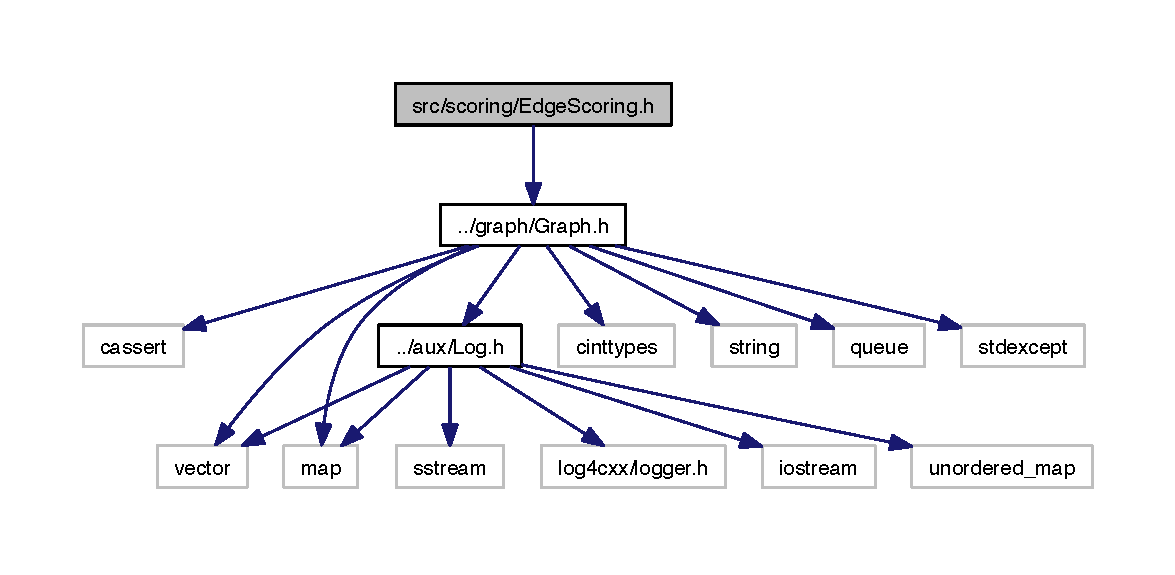
\includegraphics[width=350pt]{_edge_scoring_8h__incl}
\end{center}
\end{figure}
This graph shows which files directly or indirectly include this file\-:\nopagebreak
\begin{figure}[H]
\begin{center}
\leavevmode
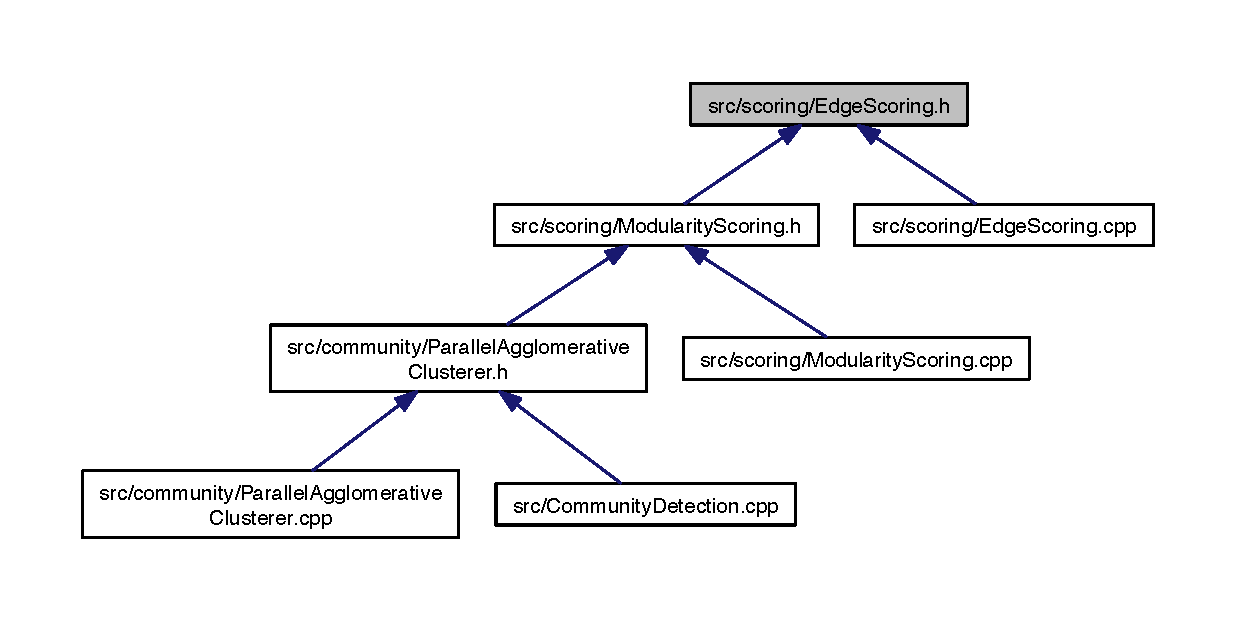
\includegraphics[width=350pt]{_edge_scoring_8h__dep__incl}
\end{center}
\end{figure}
\subsection*{Classes}
\begin{DoxyCompactItemize}
\item 
class \hyperlink{class_networ_kit_1_1_edge_scoring}{Networ\-Kit\-::\-Edge\-Scoring$<$ T $>$}
\end{DoxyCompactItemize}
\subsection*{Namespaces}
\begin{DoxyCompactItemize}
\item 
\hyperlink{namespace_networ_kit}{Networ\-Kit}
\end{DoxyCompactItemize}
\subsection*{Constant Groups}
\begin{DoxyCompactItemize}
\item 
\hyperlink{namespace_networ_kit}{Networ\-Kit}
\end{DoxyCompactItemize}

\hypertarget{_edge_triple_graph_data_8cpp}{\section{src/\-Edge\-Triple\-Graph\-Data.cpp File Reference}
\label{_edge_triple_graph_data_8cpp}\index{src/\-Edge\-Triple\-Graph\-Data.\-cpp@{src/\-Edge\-Triple\-Graph\-Data.\-cpp}}
}
{\ttfamily \#include \char`\"{}Edge\-Triple\-Graph\-Data.\-h\char`\"{}}\\*
\subsection*{Namespaces}
\begin{DoxyCompactItemize}
\item 
namespace \hyperlink{namespace_ensemble_clustering}{Ensemble\-Clustering}
\end{DoxyCompactItemize}

\hypertarget{_edge_triple_graph_data_8h}{\section{src/\-Edge\-Triple\-Graph\-Data.h File Reference}
\label{_edge_triple_graph_data_8h}\index{src/\-Edge\-Triple\-Graph\-Data.\-h@{src/\-Edge\-Triple\-Graph\-Data.\-h}}
}
\subsection*{Classes}
\begin{DoxyCompactItemize}
\item 
class \hyperlink{class_ensemble_clustering_1_1_edge_tuple}{Ensemble\-Clustering\-::\-Edge\-Tuple}
\begin{DoxyCompactList}\small\item\em \hyperlink{class_ensemble_clustering_1_1_edge_tuple}{Edge\-Tuple} contains triple (i, j, w) where i\-: edge source index j\-: edge target index w\-: edge weight. \end{DoxyCompactList}\item 
class \hyperlink{class_ensemble_clustering_1_1_node_tuple}{Ensemble\-Clustering\-::\-Node\-Tuple}
\item 
class \hyperlink{class_ensemble_clustering_1_1_edge_triple_graph_data}{Ensemble\-Clustering\-::\-Edge\-Triple\-Graph\-Data}
\end{DoxyCompactItemize}
\subsection*{Namespaces}
\begin{DoxyCompactItemize}
\item 
namespace \hyperlink{namespace_ensemble_clustering}{Ensemble\-Clustering}
\end{DoxyCompactItemize}

\hypertarget{_ensemble_clustering_8cpp}{\section{src/\-Ensemble\-Clustering.cpp File Reference}
\label{_ensemble_clustering_8cpp}\index{src/\-Ensemble\-Clustering.\-cpp@{src/\-Ensemble\-Clustering.\-cpp}}
}
{\ttfamily \#include $<$iostream$>$}\\*
{\ttfamily \#include $<$utility$>$}\\*
{\ttfamily \#include $<$unordered\-\_\-map$>$}\\*
{\ttfamily \#include \char`\"{}log4cxx/logger.\-h\char`\"{}}\\*
{\ttfamily \#include \char`\"{}log4cxx/basicconfigurator.\-h\char`\"{}}\\*
{\ttfamily \#include $<$cppunit/\-Compiler\-Outputter.\-h$>$}\\*
{\ttfamily \#include $<$cppunit/extensions/\-Test\-Factory\-Registry.\-h$>$}\\*
{\ttfamily \#include $<$cppunit/\-Test\-Result.\-h$>$}\\*
{\ttfamily \#include $<$cppunit/\-Test\-Result\-Collector.\-h$>$}\\*
{\ttfamily \#include $<$cppunit/\-Test\-Runner.\-h$>$}\\*
{\ttfamily \#include $<$cppunit/\-Brief\-Test\-Progress\-Listener.\-h$>$}\\*
{\ttfamily \#include \char`\"{}gtest/gtest.\-h\char`\"{}}\\*
{\ttfamily \#include \char`\"{}aux/log.\-h\char`\"{}}\\*
{\ttfamily \#include \char`\"{}aux/\-Noise.\-h\char`\"{}}\\*
{\ttfamily \#include \char`\"{}graph/\-Graph.\-h\char`\"{}}\\*
{\ttfamily \#include \char`\"{}input/\-M\-E\-T\-I\-S\-Parser.\-h\char`\"{}}\\*
{\ttfamily \#include \char`\"{}input/\-M\-E\-T\-I\-Sto\-S\-T\-I\-N\-G\-E\-R.\-h\char`\"{}}\\*
{\ttfamily \#include \char`\"{}matching/\-Matching.\-h\char`\"{}}\\*
{\ttfamily \#include \char`\"{}clustering/\-Clustering.\-h\char`\"{}}\\*
{\ttfamily \#include \char`\"{}clustering/\-Clustering\-Generator.\-h\char`\"{}}\\*
{\ttfamily \#include \char`\"{}graph/\-Graph\-Generator.\-h\char`\"{}}\\*
{\ttfamily \#include \char`\"{}clustering/\-Modularity.\-h\char`\"{}}\\*
{\ttfamily \#include \char`\"{}stinger.\-h\char`\"{}}\\*
Include dependency graph for Ensemble\-Clustering.\-cpp\-:\nopagebreak
\begin{figure}[H]
\begin{center}
\leavevmode
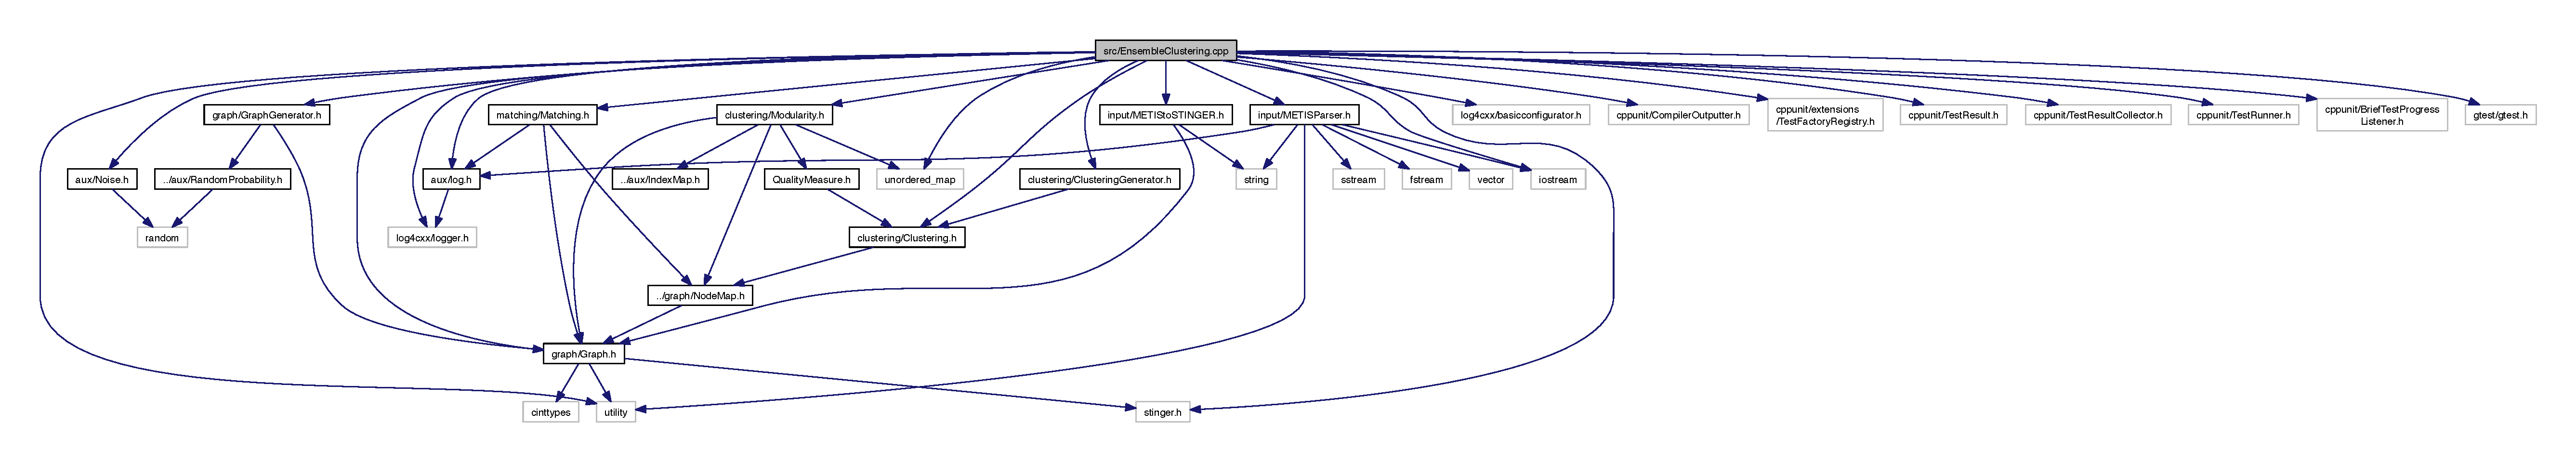
\includegraphics[width=350pt]{_ensemble_clustering_8cpp__incl}
\end{center}
\end{figure}
\subsection*{Functions}
\begin{DoxyCompactItemize}
\item 
void \hyperlink{_ensemble_clustering_8cpp_a8812968b4c432ff873e47469a09f98ed}{test\-M\-E\-T\-I\-Sto\-S\-T\-I\-N\-G\-E\-R} ()
\item 
void \hyperlink{_ensemble_clustering_8cpp_a85cffe0e678e839d43a0aaeed3f8563f}{test\-Matching} ()
\item 
\hyperlink{class_ensemble_clustering_1_1_graph}{Graph} \& \hyperlink{_ensemble_clustering_8cpp_a95ced9d3d0a7270acb5f2b3deea53ace}{make\-Complete\-Graph} (int n)
\begin{DoxyCompactList}\small\item\em Make a complete graph with n vertices. \end{DoxyCompactList}\item 
void \hyperlink{_ensemble_clustering_8cpp_a743dc80157d90a093ae489a586acfae7}{configure\-Logging} ()
\begin{DoxyCompactList}\small\item\em Call this first to configure logging output. \end{DoxyCompactList}\item 
int \hyperlink{_ensemble_clustering_8cpp_a3c04138a5bfe5d72780bb7e82a18e627}{main} (int argc, char $\ast$$\ast$argv)
\end{DoxyCompactItemize}


\subsection{Function Documentation}
\hypertarget{_ensemble_clustering_8cpp_a743dc80157d90a093ae489a586acfae7}{\index{Ensemble\-Clustering.\-cpp@{Ensemble\-Clustering.\-cpp}!configure\-Logging@{configure\-Logging}}
\index{configure\-Logging@{configure\-Logging}!EnsembleClustering.cpp@{Ensemble\-Clustering.\-cpp}}
\subsubsection[{configure\-Logging}]{\setlength{\rightskip}{0pt plus 5cm}void configure\-Logging (
\begin{DoxyParamCaption}
{}
\end{DoxyParamCaption}
)}}\label{_ensemble_clustering_8cpp_a743dc80157d90a093ae489a586acfae7}


Call this first to configure logging output. 



Definition at line 112 of file Ensemble\-Clustering.\-cpp.

\hypertarget{_ensemble_clustering_8cpp_a3c04138a5bfe5d72780bb7e82a18e627}{\index{Ensemble\-Clustering.\-cpp@{Ensemble\-Clustering.\-cpp}!main@{main}}
\index{main@{main}!EnsembleClustering.cpp@{Ensemble\-Clustering.\-cpp}}
\subsubsection[{main}]{\setlength{\rightskip}{0pt plus 5cm}int main (
\begin{DoxyParamCaption}
\item[{int}]{argc, }
\item[{char $\ast$$\ast$}]{argv}
\end{DoxyParamCaption}
)}}\label{_ensemble_clustering_8cpp_a3c04138a5bfe5d72780bb7e82a18e627}


Definition at line 121 of file Ensemble\-Clustering.\-cpp.



Here is the call graph for this function\-:\nopagebreak
\begin{figure}[H]
\begin{center}
\leavevmode
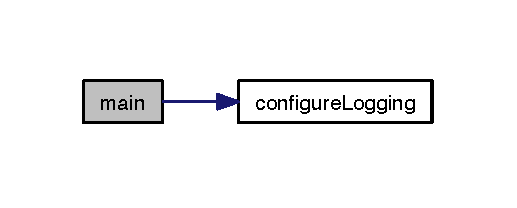
\includegraphics[width=248pt]{_ensemble_clustering_8cpp_a3c04138a5bfe5d72780bb7e82a18e627_cgraph}
\end{center}
\end{figure}


\hypertarget{_ensemble_clustering_8cpp_a95ced9d3d0a7270acb5f2b3deea53ace}{\index{Ensemble\-Clustering.\-cpp@{Ensemble\-Clustering.\-cpp}!make\-Complete\-Graph@{make\-Complete\-Graph}}
\index{make\-Complete\-Graph@{make\-Complete\-Graph}!EnsembleClustering.cpp@{Ensemble\-Clustering.\-cpp}}
\subsubsection[{make\-Complete\-Graph}]{\setlength{\rightskip}{0pt plus 5cm}{\bf Graph}\& make\-Complete\-Graph (
\begin{DoxyParamCaption}
\item[{int}]{n}
\end{DoxyParamCaption}
)}}\label{_ensemble_clustering_8cpp_a95ced9d3d0a7270acb5f2b3deea53ace}


Make a complete graph with n vertices. 



Definition at line 93 of file Ensemble\-Clustering.\-cpp.



Here is the call graph for this function\-:\nopagebreak
\begin{figure}[H]
\begin{center}
\leavevmode
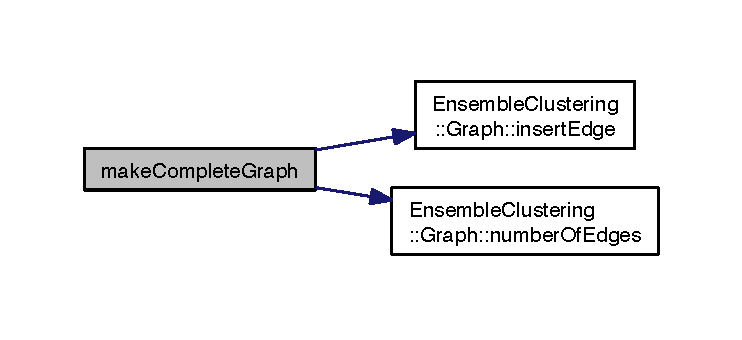
\includegraphics[width=350pt]{_ensemble_clustering_8cpp_a95ced9d3d0a7270acb5f2b3deea53ace_cgraph}
\end{center}
\end{figure}


\hypertarget{_ensemble_clustering_8cpp_a85cffe0e678e839d43a0aaeed3f8563f}{\index{Ensemble\-Clustering.\-cpp@{Ensemble\-Clustering.\-cpp}!test\-Matching@{test\-Matching}}
\index{test\-Matching@{test\-Matching}!EnsembleClustering.cpp@{Ensemble\-Clustering.\-cpp}}
\subsubsection[{test\-Matching}]{\setlength{\rightskip}{0pt plus 5cm}void test\-Matching (
\begin{DoxyParamCaption}
{}
\end{DoxyParamCaption}
)}}\label{_ensemble_clustering_8cpp_a85cffe0e678e839d43a0aaeed3f8563f}


Definition at line 70 of file Ensemble\-Clustering.\-cpp.



Here is the call graph for this function\-:\nopagebreak
\begin{figure}[H]
\begin{center}
\leavevmode
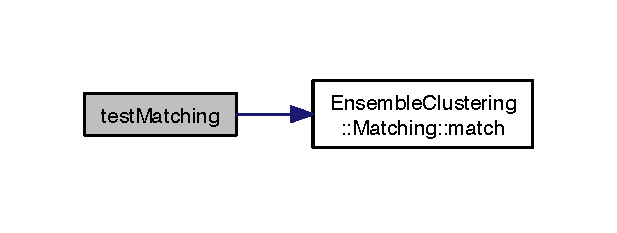
\includegraphics[width=296pt]{_ensemble_clustering_8cpp_a85cffe0e678e839d43a0aaeed3f8563f_cgraph}
\end{center}
\end{figure}


\hypertarget{_ensemble_clustering_8cpp_a8812968b4c432ff873e47469a09f98ed}{\index{Ensemble\-Clustering.\-cpp@{Ensemble\-Clustering.\-cpp}!test\-M\-E\-T\-I\-Sto\-S\-T\-I\-N\-G\-E\-R@{test\-M\-E\-T\-I\-Sto\-S\-T\-I\-N\-G\-E\-R}}
\index{test\-M\-E\-T\-I\-Sto\-S\-T\-I\-N\-G\-E\-R@{test\-M\-E\-T\-I\-Sto\-S\-T\-I\-N\-G\-E\-R}!EnsembleClustering.cpp@{Ensemble\-Clustering.\-cpp}}
\subsubsection[{test\-M\-E\-T\-I\-Sto\-S\-T\-I\-N\-G\-E\-R}]{\setlength{\rightskip}{0pt plus 5cm}void test\-M\-E\-T\-I\-Sto\-S\-T\-I\-N\-G\-E\-R (
\begin{DoxyParamCaption}
{}
\end{DoxyParamCaption}
)}}\label{_ensemble_clustering_8cpp_a8812968b4c432ff873e47469a09f98ed}


Definition at line 53 of file Ensemble\-Clustering.\-cpp.



Here is the call graph for this function\-:\nopagebreak
\begin{figure}[H]
\begin{center}
\leavevmode
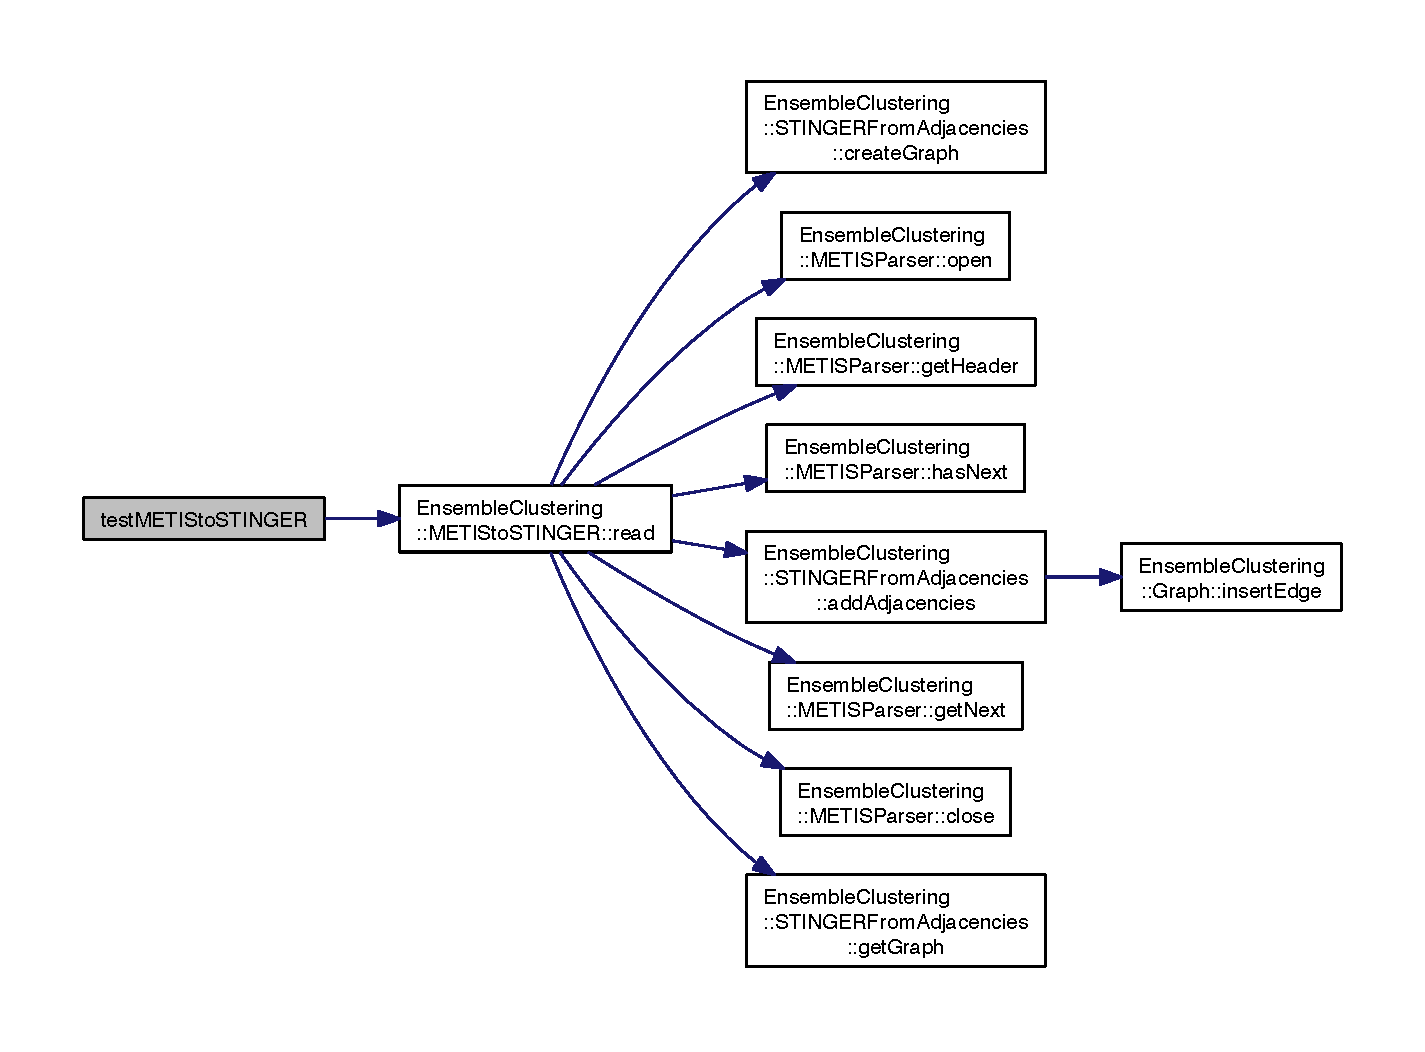
\includegraphics[width=350pt]{_ensemble_clustering_8cpp_a8812968b4c432ff873e47469a09f98ed_cgraph}
\end{center}
\end{figure}



\hypertarget{_ensemble_clustering_algo_8cpp}{\section{src/\-Ensemble\-Clustering\-Algo.cpp File Reference}
\label{_ensemble_clustering_algo_8cpp}\index{src/\-Ensemble\-Clustering\-Algo.\-cpp@{src/\-Ensemble\-Clustering\-Algo.\-cpp}}
}
{\ttfamily \#include \char`\"{}Ensemble\-Clustering\-Algo.\-h\char`\"{}}\\*
\subsection*{Namespaces}
\begin{DoxyCompactItemize}
\item 
namespace \hyperlink{namespace_ensemble_clustering}{Ensemble\-Clustering}
\end{DoxyCompactItemize}

\hypertarget{_ensemble_clustering_algo_8h}{\section{src/\-Ensemble\-Clustering\-Algo.h File Reference}
\label{_ensemble_clustering_algo_8h}\index{src/\-Ensemble\-Clustering\-Algo.\-h@{src/\-Ensemble\-Clustering\-Algo.\-h}}
}
\subsection*{Classes}
\begin{DoxyCompactItemize}
\item 
class \hyperlink{class_ensemble_clustering_1_1_ensemble_clustering_algo}{Ensemble\-Clustering\-::\-Ensemble\-Clustering\-Algo}
\end{DoxyCompactItemize}
\subsection*{Namespaces}
\begin{DoxyCompactItemize}
\item 
namespace \hyperlink{namespace_ensemble_clustering}{Ensemble\-Clustering}
\end{DoxyCompactItemize}

\hypertarget{_graph_8cpp}{\section{src/graph/\-Graph.cpp File Reference}
\label{_graph_8cpp}\index{src/graph/\-Graph.\-cpp@{src/graph/\-Graph.\-cpp}}
}
{\ttfamily \#include \char`\"{}Graph.\-h\char`\"{}}\\*
Include dependency graph for Graph.\-cpp\-:\nopagebreak
\begin{figure}[H]
\begin{center}
\leavevmode
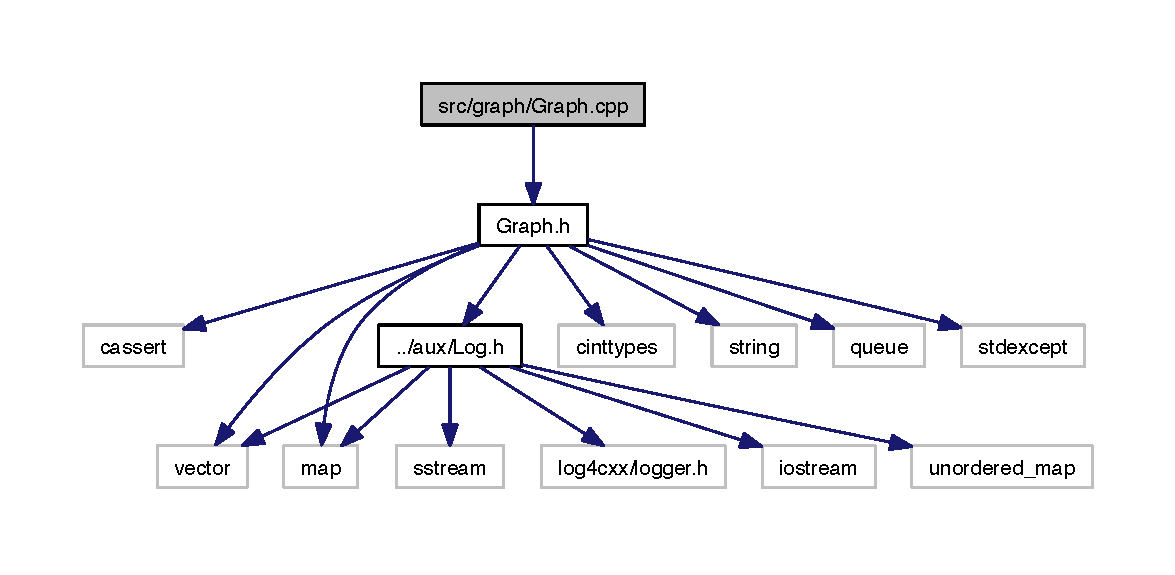
\includegraphics[width=350pt]{_graph_8cpp__incl}
\end{center}
\end{figure}
\subsection*{Namespaces}
\begin{DoxyCompactItemize}
\item 
namespace \hyperlink{namespace_networ_kit}{Networ\-Kit}
\end{DoxyCompactItemize}

\hypertarget{_graph_8h}{\section{src/graph/\-Graph.h File Reference}
\label{_graph_8h}\index{src/graph/\-Graph.\-h@{src/graph/\-Graph.\-h}}
}
{\ttfamily \#include $<$cassert$>$}\\*
{\ttfamily \#include $<$vector$>$}\\*
{\ttfamily \#include $<$cinttypes$>$}\\*
{\ttfamily \#include $<$string$>$}\\*
{\ttfamily \#include $<$queue$>$}\\*
{\ttfamily \#include $<$stdexcept$>$}\\*
{\ttfamily \#include $<$map$>$}\\*
{\ttfamily \#include \char`\"{}../aux/\-Log.\-h\char`\"{}}\\*
Include dependency graph for Graph.\-h\-:\nopagebreak
\begin{figure}[H]
\begin{center}
\leavevmode
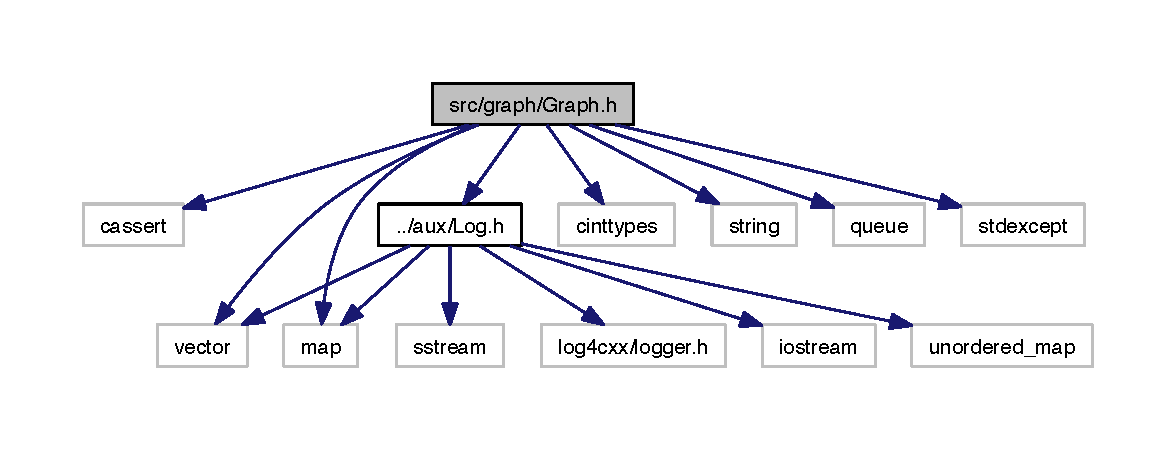
\includegraphics[width=350pt]{_graph_8h__incl}
\end{center}
\end{figure}
This graph shows which files directly or indirectly include this file\-:\nopagebreak
\begin{figure}[H]
\begin{center}
\leavevmode
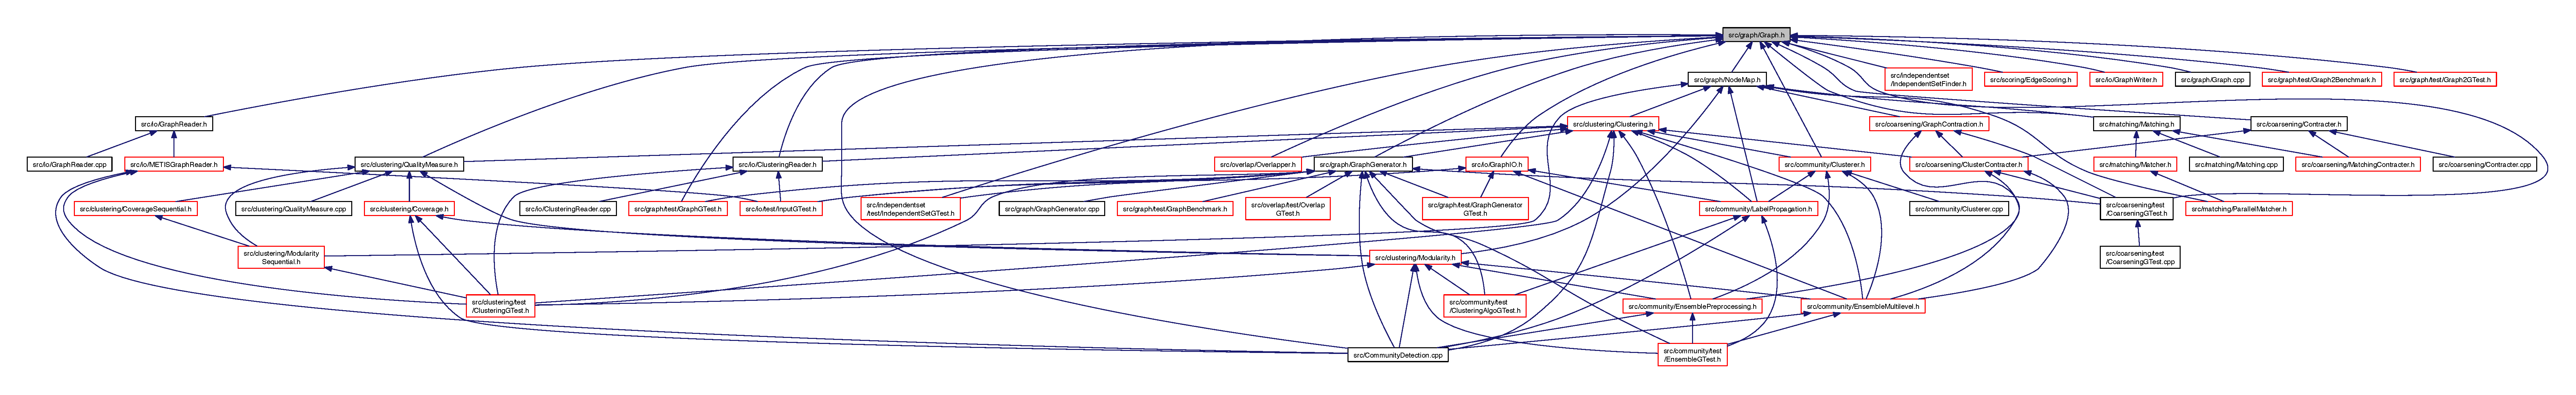
\includegraphics[width=350pt]{_graph_8h__dep__incl}
\end{center}
\end{figure}
\subsection*{Classes}
\begin{DoxyCompactItemize}
\item 
class \hyperlink{class_networ_kit_1_1_graph}{Networ\-Kit\-::\-Graph}
\item 
class \hyperlink{class_networ_kit_1_1_graph_1_1_node_attribute}{Networ\-Kit\-::\-Graph\-::\-Node\-Attribute}
\begin{DoxyCompactList}\small\item\em A\-T\-T\-R\-I\-B\-U\-T\-E A\-B\-S\-T\-R\-A\-C\-T B\-A\-S\-E C\-L\-A\-S\-S\-E\-S. \end{DoxyCompactList}\item 
class \hyperlink{class_networ_kit_1_1_graph_1_1_edge_attribute}{Networ\-Kit\-::\-Graph\-::\-Edge\-Attribute}
\end{DoxyCompactItemize}
\subsection*{Namespaces}
\begin{DoxyCompactItemize}
\item 
namespace \hyperlink{namespace_networ_kit}{Networ\-Kit}
\end{DoxyCompactItemize}
\subsection*{Macros}
\begin{DoxyCompactItemize}
\item 
\#define \hyperlink{_graph_8h_a7c01eac0d89b74473a90fd5c33ed4e74}{none}~-\/1
\end{DoxyCompactItemize}
\subsection*{Typedefs}
\begin{DoxyCompactItemize}
\item 
typedef int64\-\_\-t \hyperlink{namespace_networ_kit_af49e67df68af41dcd75dffbb1e9abee6}{Networ\-Kit\-::index}
\begin{DoxyCompactList}\small\item\em Typedefs. \end{DoxyCompactList}\item 
typedef int64\-\_\-t \hyperlink{namespace_networ_kit_ad4c536a5339a8bf2f91f418b9a67a7d8}{Networ\-Kit\-::count}
\item 
typedef index \hyperlink{namespace_networ_kit_a61914158fd771265be48de9942369160}{Networ\-Kit\-::node}
\item 
typedef double \hyperlink{namespace_networ_kit_a831b108dbcd79dad062d9e28b1b4e3dd}{Networ\-Kit\-::edgeweight}
\end{DoxyCompactItemize}


\subsection{Macro Definition Documentation}
\hypertarget{_graph_8h_a7c01eac0d89b74473a90fd5c33ed4e74}{\index{Graph.\-h@{Graph.\-h}!none@{none}}
\index{none@{none}!Graph.h@{Graph.\-h}}
\subsubsection[{none}]{\setlength{\rightskip}{0pt plus 5cm}\#define none~-\/1}}\label{_graph_8h_a7c01eac0d89b74473a90fd5c33ed4e74}


Definition at line 21 of file Graph.\-h.


\hypertarget{_matching_8cpp}{\section{src/matching/\-Matching.cpp File Reference}
\label{_matching_8cpp}\index{src/matching/\-Matching.\-cpp@{src/matching/\-Matching.\-cpp}}
}
{\ttfamily \#include \char`\"{}Matching.\-h\char`\"{}}\\*
Include dependency graph for Matching.\-cpp\-:\nopagebreak
\begin{figure}[H]
\begin{center}
\leavevmode
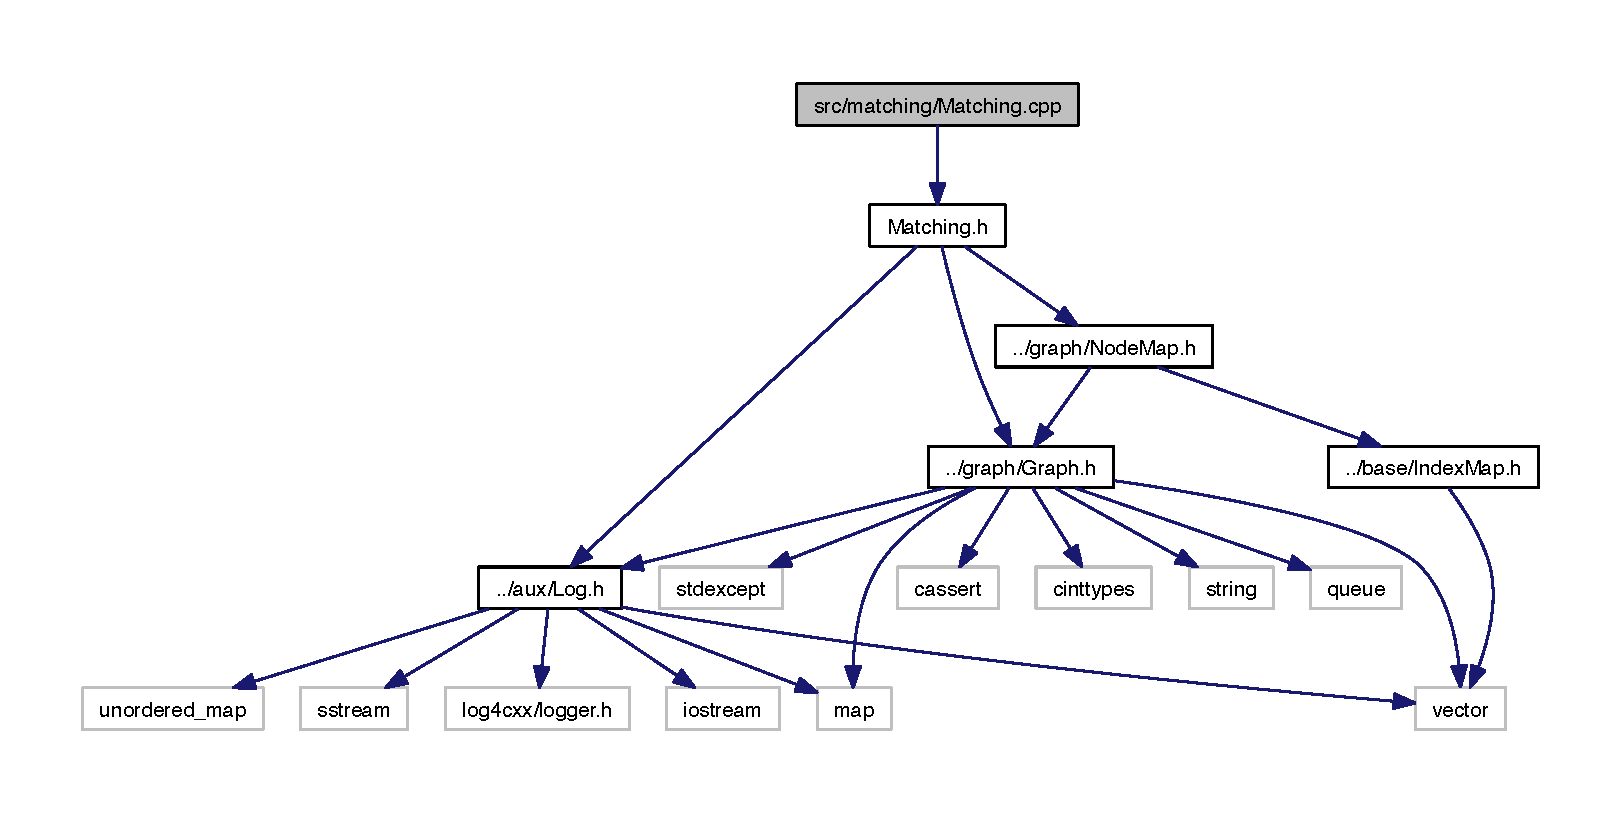
\includegraphics[width=350pt]{_matching_8cpp__incl}
\end{center}
\end{figure}
\subsection*{Namespaces}
\begin{DoxyCompactItemize}
\item 
namespace \hyperlink{namespace_networ_kit}{Networ\-Kit}
\end{DoxyCompactItemize}

\hypertarget{_matching_8h}{\section{src/matching/\-Matching.h File Reference}
\label{_matching_8h}\index{src/matching/\-Matching.\-h@{src/matching/\-Matching.\-h}}
}
{\ttfamily \#include \char`\"{}../aux/\-Log.\-h\char`\"{}}\\*
{\ttfamily \#include \char`\"{}../graph/\-Graph.\-h\char`\"{}}\\*
{\ttfamily \#include \char`\"{}../graph/\-Node\-Map.\-h\char`\"{}}\\*
Include dependency graph for Matching.\-h\-:\nopagebreak
\begin{figure}[H]
\begin{center}
\leavevmode
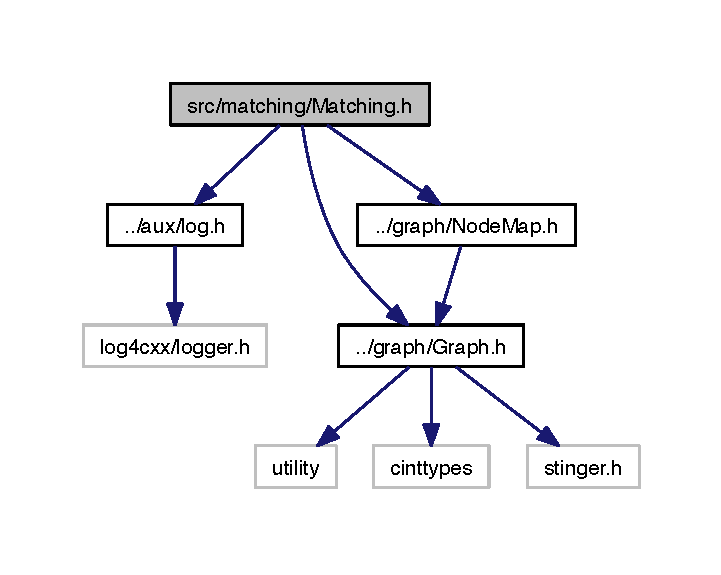
\includegraphics[width=350pt]{_matching_8h__incl}
\end{center}
\end{figure}
This graph shows which files directly or indirectly include this file\-:\nopagebreak
\begin{figure}[H]
\begin{center}
\leavevmode
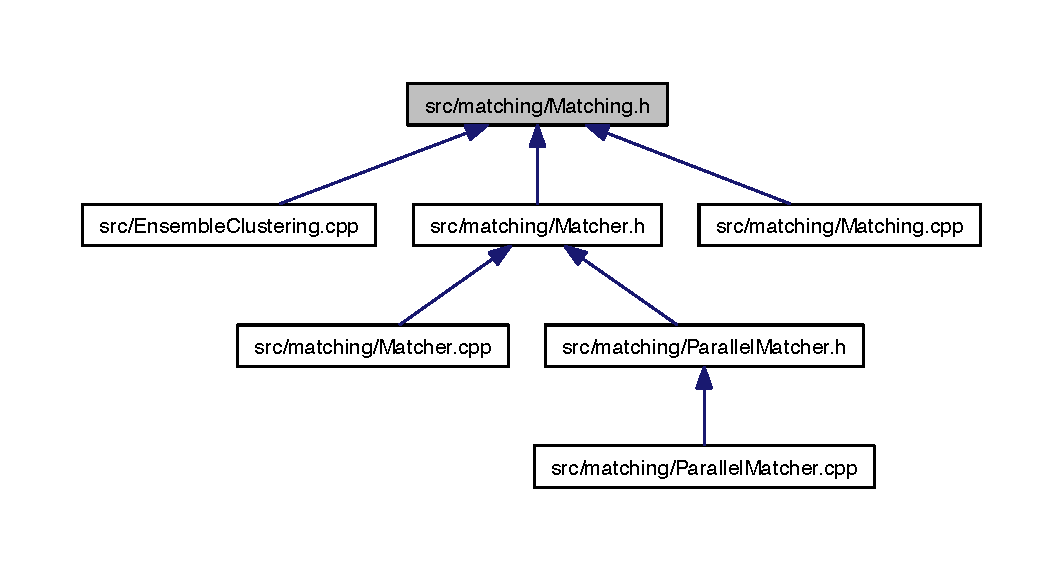
\includegraphics[width=350pt]{_matching_8h__dep__incl}
\end{center}
\end{figure}
\subsection*{Classes}
\begin{DoxyCompactItemize}
\item 
class \hyperlink{class_networ_kit_1_1_matching}{Networ\-Kit\-::\-Matching}
\end{DoxyCompactItemize}
\subsection*{Namespaces}
\begin{DoxyCompactItemize}
\item 
namespace \hyperlink{namespace_networ_kit}{Networ\-Kit}
\end{DoxyCompactItemize}

\hypertarget{_m_e_t_i_s_graph_parser_8cpp}{\section{src/\-M\-E\-T\-I\-S\-Graph\-Parser.cpp File Reference}
\label{_m_e_t_i_s_graph_parser_8cpp}\index{src/\-M\-E\-T\-I\-S\-Graph\-Parser.\-cpp@{src/\-M\-E\-T\-I\-S\-Graph\-Parser.\-cpp}}
}
{\ttfamily \#include \char`\"{}M\-E\-T\-I\-S\-Graph\-Parser.\-h\char`\"{}}\\*
{\ttfamily \#include $<$fstream$>$}\\*
{\ttfamily \#include $<$vector$>$}\\*
{\ttfamily \#include $<$string$>$}\\*
{\ttfamily \#include $<$sstream$>$}\\*
{\ttfamily \#include \char`\"{}Edge\-Triple\-Graph\-Data.\-h\char`\"{}}\\*
\subsection*{Namespaces}
\begin{DoxyCompactItemize}
\item 
namespace \hyperlink{namespace_ensemble_clustering}{Ensemble\-Clustering}
\end{DoxyCompactItemize}

\hypertarget{_m_e_t_i_s_graph_parser_8h}{\section{src/\-M\-E\-T\-I\-S\-Graph\-Parser.h File Reference}
\label{_m_e_t_i_s_graph_parser_8h}\index{src/\-M\-E\-T\-I\-S\-Graph\-Parser.\-h@{src/\-M\-E\-T\-I\-S\-Graph\-Parser.\-h}}
}
{\ttfamily \#include $<$iostream$>$}\\*
{\ttfamily \#include $<$vector$>$}\\*
{\ttfamily \#include \char`\"{}Graph.\-h\char`\"{}}\\*
{\ttfamily \#include \char`\"{}Edge\-Triple\-Graph\-Data.\-h\char`\"{}}\\*
\subsection*{Classes}
\begin{DoxyCompactItemize}
\item 
class \hyperlink{class_ensemble_clustering_1_1_m_e_t_i_s_graph_parser}{Ensemble\-Clustering\-::\-M\-E\-T\-I\-S\-Graph\-Parser}
\begin{DoxyCompactList}\small\item\em A parser for the M\-E\-T\-I\-S graph file format. \end{DoxyCompactList}\end{DoxyCompactItemize}
\subsection*{Namespaces}
\begin{DoxyCompactItemize}
\item 
namespace \hyperlink{namespace_ensemble_clustering}{Ensemble\-Clustering}
\end{DoxyCompactItemize}
\subsection*{Typedefs}
\begin{DoxyCompactItemize}
\item 
typedef unsigned int \hyperlink{namespace_ensemble_clustering_a3228848abf8dfd6602f3b08dd459ea20}{Ensemble\-Clustering\-::id}
\end{DoxyCompactItemize}

\hypertarget{_modularity_8cpp}{\section{src/\-Modularity.cpp File Reference}
\label{_modularity_8cpp}\index{src/\-Modularity.\-cpp@{src/\-Modularity.\-cpp}}
}
{\ttfamily \#include \char`\"{}Modularity.\-h\char`\"{}}\\*
\subsection*{Namespaces}
\begin{DoxyCompactItemize}
\item 
namespace \hyperlink{namespace_ensemble_clustering}{Ensemble\-Clustering}
\end{DoxyCompactItemize}

\hypertarget{_modularity_8h}{\section{src/clustering/\-Modularity.h File Reference}
\label{_modularity_8h}\index{src/clustering/\-Modularity.\-h@{src/clustering/\-Modularity.\-h}}
}
{\ttfamily \#include $<$unordered\-\_\-map$>$}\\*
{\ttfamily \#include $<$cmath$>$}\\*
{\ttfamily \#include $<$stdexcept$>$}\\*
{\ttfamily \#include \char`\"{}Quality\-Measure.\-h\char`\"{}}\\*
{\ttfamily \#include \char`\"{}Coverage.\-h\char`\"{}}\\*
{\ttfamily \#include \char`\"{}../base/\-Index\-Map.\-h\char`\"{}}\\*
{\ttfamily \#include \char`\"{}../graph/\-Node\-Map.\-h\char`\"{}}\\*
Include dependency graph for Modularity.\-h\-:\nopagebreak
\begin{figure}[H]
\begin{center}
\leavevmode
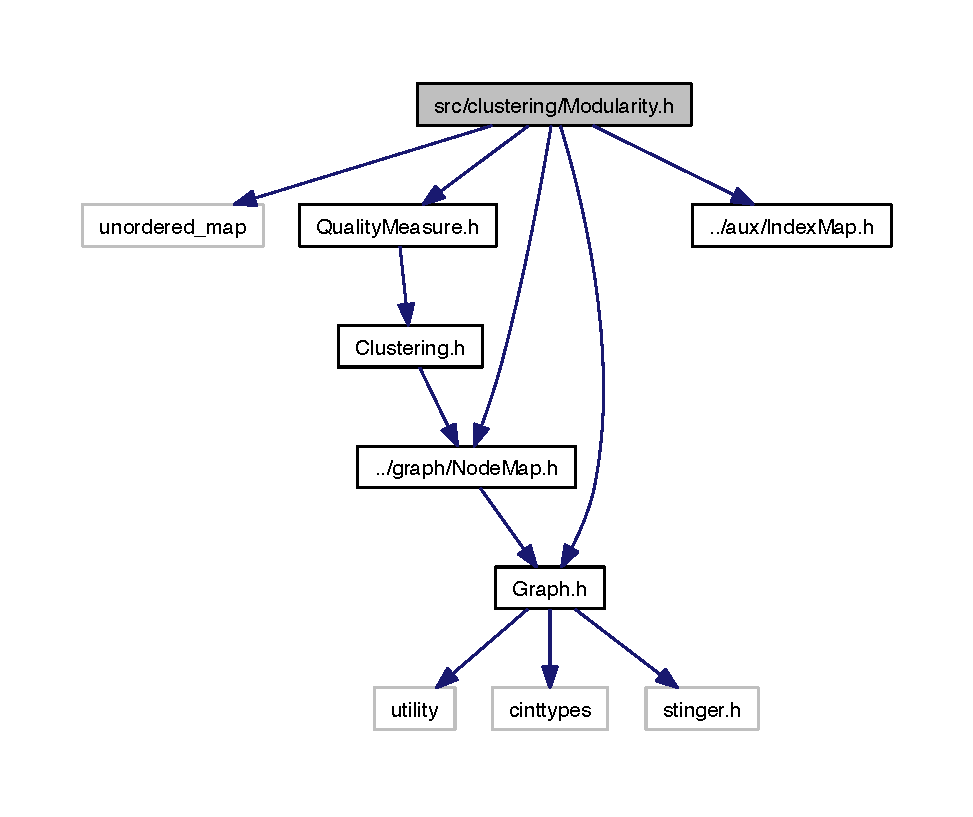
\includegraphics[width=350pt]{_modularity_8h__incl}
\end{center}
\end{figure}
This graph shows which files directly or indirectly include this file\-:\nopagebreak
\begin{figure}[H]
\begin{center}
\leavevmode
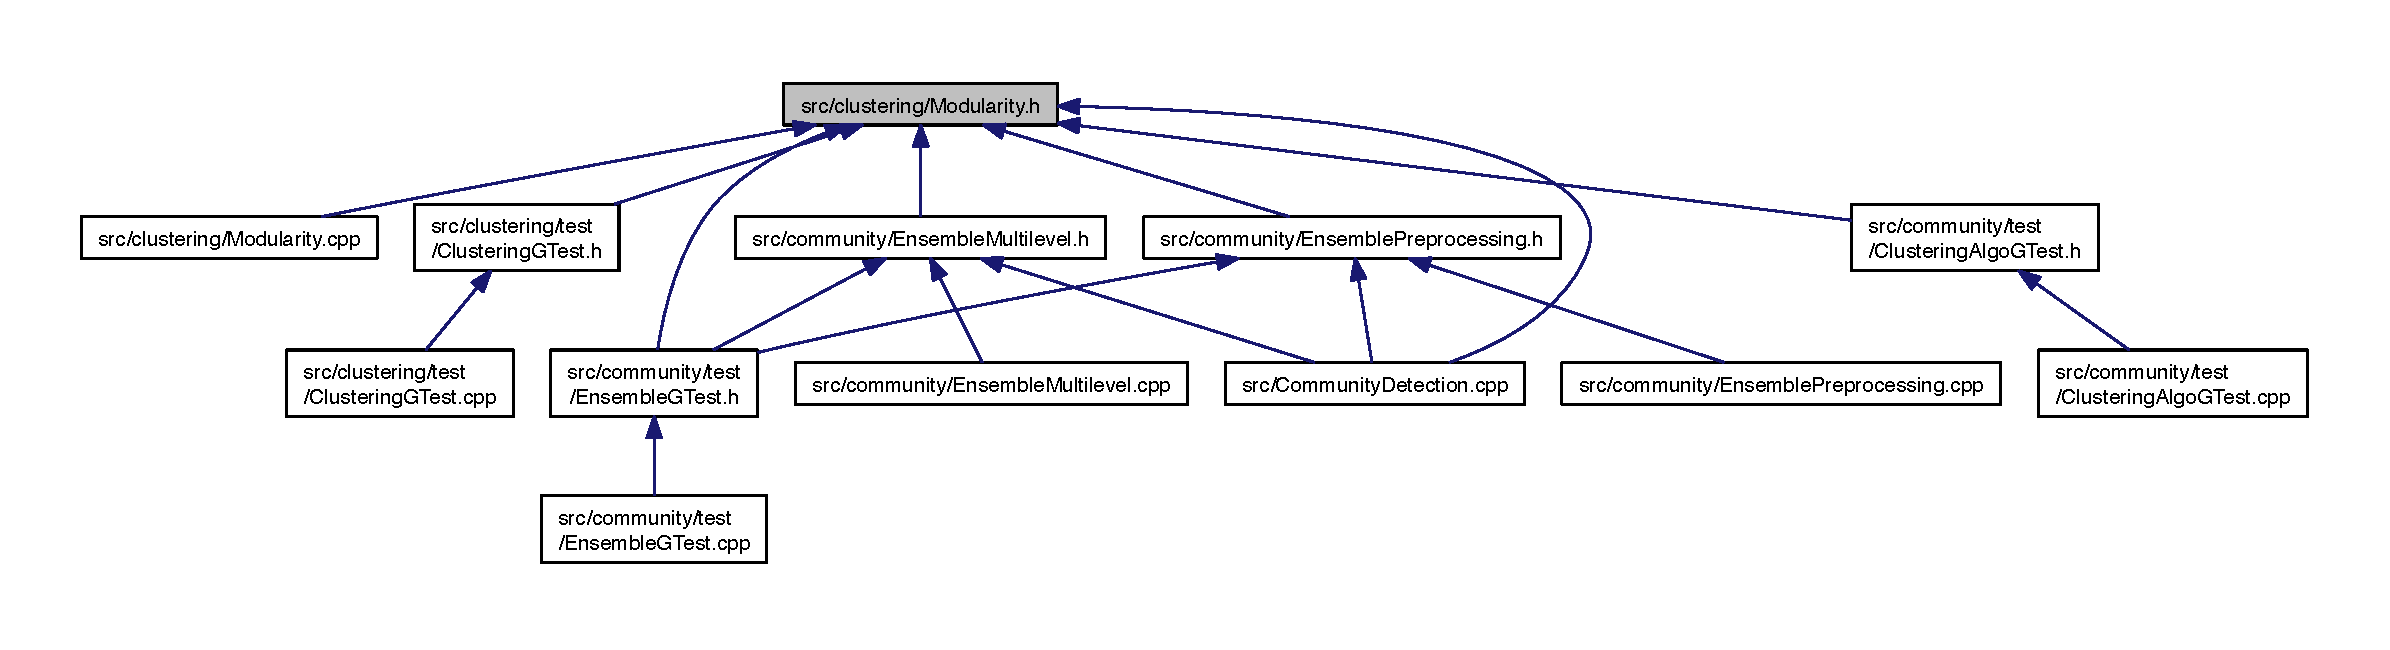
\includegraphics[width=350pt]{_modularity_8h__dep__incl}
\end{center}
\end{figure}
\subsection*{Classes}
\begin{DoxyCompactItemize}
\item 
class \hyperlink{class_networ_kit_1_1_modularity}{Networ\-Kit\-::\-Modularity}
\end{DoxyCompactItemize}
\subsection*{Namespaces}
\begin{DoxyCompactItemize}
\item 
\hyperlink{namespace_networ_kit}{Networ\-Kit}
\end{DoxyCompactItemize}
\subsection*{Constant Groups}
\begin{DoxyCompactItemize}
\item 
\hyperlink{namespace_networ_kit}{Networ\-Kit}
\end{DoxyCompactItemize}

\addcontentsline{toc}{part}{Index}
\printindex
\end{document}
